% Options for packages loaded elsewhere
\PassOptionsToPackage{unicode}{hyperref}
\PassOptionsToPackage{hyphens}{url}
%
\documentclass[
]{book}
\usepackage{amsmath,amssymb}
\usepackage{lmodern}
\usepackage{iftex}
\ifPDFTeX
  \usepackage[T1]{fontenc}
  \usepackage[utf8]{inputenc}
  \usepackage{textcomp} % provide euro and other symbols
\else % if luatex or xetex
  \usepackage{unicode-math}
  \defaultfontfeatures{Scale=MatchLowercase}
  \defaultfontfeatures[\rmfamily]{Ligatures=TeX,Scale=1}
\fi
% Use upquote if available, for straight quotes in verbatim environments
\IfFileExists{upquote.sty}{\usepackage{upquote}}{}
\IfFileExists{microtype.sty}{% use microtype if available
  \usepackage[]{microtype}
  \UseMicrotypeSet[protrusion]{basicmath} % disable protrusion for tt fonts
}{}
\makeatletter
\@ifundefined{KOMAClassName}{% if non-KOMA class
  \IfFileExists{parskip.sty}{%
    \usepackage{parskip}
  }{% else
    \setlength{\parindent}{0pt}
    \setlength{\parskip}{6pt plus 2pt minus 1pt}}
}{% if KOMA class
  \KOMAoptions{parskip=half}}
\makeatother
\usepackage{xcolor}
\usepackage{color}
\usepackage{fancyvrb}
\newcommand{\VerbBar}{|}
\newcommand{\VERB}{\Verb[commandchars=\\\{\}]}
\DefineVerbatimEnvironment{Highlighting}{Verbatim}{commandchars=\\\{\}}
% Add ',fontsize=\small' for more characters per line
\usepackage{framed}
\definecolor{shadecolor}{RGB}{248,248,248}
\newenvironment{Shaded}{\begin{snugshade}}{\end{snugshade}}
\newcommand{\AlertTok}[1]{\textcolor[rgb]{0.94,0.16,0.16}{#1}}
\newcommand{\AnnotationTok}[1]{\textcolor[rgb]{0.56,0.35,0.01}{\textbf{\textit{#1}}}}
\newcommand{\AttributeTok}[1]{\textcolor[rgb]{0.77,0.63,0.00}{#1}}
\newcommand{\BaseNTok}[1]{\textcolor[rgb]{0.00,0.00,0.81}{#1}}
\newcommand{\BuiltInTok}[1]{#1}
\newcommand{\CharTok}[1]{\textcolor[rgb]{0.31,0.60,0.02}{#1}}
\newcommand{\CommentTok}[1]{\textcolor[rgb]{0.56,0.35,0.01}{\textit{#1}}}
\newcommand{\CommentVarTok}[1]{\textcolor[rgb]{0.56,0.35,0.01}{\textbf{\textit{#1}}}}
\newcommand{\ConstantTok}[1]{\textcolor[rgb]{0.00,0.00,0.00}{#1}}
\newcommand{\ControlFlowTok}[1]{\textcolor[rgb]{0.13,0.29,0.53}{\textbf{#1}}}
\newcommand{\DataTypeTok}[1]{\textcolor[rgb]{0.13,0.29,0.53}{#1}}
\newcommand{\DecValTok}[1]{\textcolor[rgb]{0.00,0.00,0.81}{#1}}
\newcommand{\DocumentationTok}[1]{\textcolor[rgb]{0.56,0.35,0.01}{\textbf{\textit{#1}}}}
\newcommand{\ErrorTok}[1]{\textcolor[rgb]{0.64,0.00,0.00}{\textbf{#1}}}
\newcommand{\ExtensionTok}[1]{#1}
\newcommand{\FloatTok}[1]{\textcolor[rgb]{0.00,0.00,0.81}{#1}}
\newcommand{\FunctionTok}[1]{\textcolor[rgb]{0.00,0.00,0.00}{#1}}
\newcommand{\ImportTok}[1]{#1}
\newcommand{\InformationTok}[1]{\textcolor[rgb]{0.56,0.35,0.01}{\textbf{\textit{#1}}}}
\newcommand{\KeywordTok}[1]{\textcolor[rgb]{0.13,0.29,0.53}{\textbf{#1}}}
\newcommand{\NormalTok}[1]{#1}
\newcommand{\OperatorTok}[1]{\textcolor[rgb]{0.81,0.36,0.00}{\textbf{#1}}}
\newcommand{\OtherTok}[1]{\textcolor[rgb]{0.56,0.35,0.01}{#1}}
\newcommand{\PreprocessorTok}[1]{\textcolor[rgb]{0.56,0.35,0.01}{\textit{#1}}}
\newcommand{\RegionMarkerTok}[1]{#1}
\newcommand{\SpecialCharTok}[1]{\textcolor[rgb]{0.00,0.00,0.00}{#1}}
\newcommand{\SpecialStringTok}[1]{\textcolor[rgb]{0.31,0.60,0.02}{#1}}
\newcommand{\StringTok}[1]{\textcolor[rgb]{0.31,0.60,0.02}{#1}}
\newcommand{\VariableTok}[1]{\textcolor[rgb]{0.00,0.00,0.00}{#1}}
\newcommand{\VerbatimStringTok}[1]{\textcolor[rgb]{0.31,0.60,0.02}{#1}}
\newcommand{\WarningTok}[1]{\textcolor[rgb]{0.56,0.35,0.01}{\textbf{\textit{#1}}}}
\usepackage{longtable,booktabs,array}
\usepackage{calc} % for calculating minipage widths
% Correct order of tables after \paragraph or \subparagraph
\usepackage{etoolbox}
\makeatletter
\patchcmd\longtable{\par}{\if@noskipsec\mbox{}\fi\par}{}{}
\makeatother
% Allow footnotes in longtable head/foot
\IfFileExists{footnotehyper.sty}{\usepackage{footnotehyper}}{\usepackage{footnote}}
\makesavenoteenv{longtable}
\usepackage{graphicx}
\makeatletter
\def\maxwidth{\ifdim\Gin@nat@width>\linewidth\linewidth\else\Gin@nat@width\fi}
\def\maxheight{\ifdim\Gin@nat@height>\textheight\textheight\else\Gin@nat@height\fi}
\makeatother
% Scale images if necessary, so that they will not overflow the page
% margins by default, and it is still possible to overwrite the defaults
% using explicit options in \includegraphics[width, height, ...]{}
\setkeys{Gin}{width=\maxwidth,height=\maxheight,keepaspectratio}
% Set default figure placement to htbp
\makeatletter
\def\fps@figure{htbp}
\makeatother
\setlength{\emergencystretch}{3em} % prevent overfull lines
\providecommand{\tightlist}{%
  \setlength{\itemsep}{0pt}\setlength{\parskip}{0pt}}
\setcounter{secnumdepth}{5}
\usepackage{booktabs}
\ifLuaTeX
  \usepackage{selnolig}  % disable illegal ligatures
\fi
\usepackage[]{natbib}
\bibliographystyle{plainnat}
\IfFileExists{bookmark.sty}{\usepackage{bookmark}}{\usepackage{hyperref}}
\IfFileExists{xurl.sty}{\usepackage{xurl}}{} % add URL line breaks if available
\urlstyle{same} % disable monospaced font for URLs
\hypersetup{
  pdftitle={Applying Network Analysis to Humanities},
  pdfauthor={Yann Ryan, Iiro Tihonen},
  hidelinks,
  pdfcreator={LaTeX via pandoc}}

\title{Applying Network Analysis to Humanities}
\author{Yann Ryan, Iiro Tihonen}
\date{2022-10-26}

\begin{document}
\maketitle

{
\setcounter{tocdepth}{1}
\tableofcontents
}
\hypertarget{about-this-book}{%
\chapter{About this Book}\label{about-this-book}}

This book is intended to be read alongside the the ``Applying Network
Analysis to Humanities' course at the University of Helsinki, beginning
November 2022. This course is aimed at complete beginners to both R and
network analysis, although you'll still get plenty out of it if you have
experience with either.

It focuses on \textbf{applied approaches} to network analysis and humanities
data. Rather than cover network science in exhaustive detail, you'll
learn how to \textbf{find}, \textbf{extract}, \textbf{clean}, \textbf{visualise}, and
\textbf{analyse} humanities and cultural datasets from a network perspective.
Additionally, we'll focus on the \textbf{problems} and \textbf{pitfalls} of using
networks, specific to humanities data.

There are two chapters for each week, one for each session. Browse
through the chapters using the menu to the left.

For most classes, there is an equivalent set of exercises. We'll begin
them during the class but they can be completed afterwards. You'll
probably want to have this book at hand to complete them. They are
available as R markdown notebooks, using the \href{https://notebooks.rahtiapp.fi/welcome}{CSC notebooks
service}. You'll need a CSC
account, and you'll be sent a join code at the beginning of the course.
If you don't have either of these things, contact the \href{mailto:yann.ryan@helinki.fi}{course
leader}.

\hypertarget{about-the-course}{%
\section{About the course}\label{about-the-course}}

The course is held online, via Zoom, on Wednesdays and Fridays, between
08.15 and 09.45, starting on November 02.

Assessment is the following:

\begin{itemize}
\item
  Completion of weekly assignments (pass/fail, carried out during
  class and finished afterwards if necessary).
\item
  Presentation on final project (1/5 of the grade)\textbf{, given on
  Wednesday or Friday of the final week.}
\item
  Final project (4/5 of the grade, s\textbf{ubmitted on January 17 at the
  latest.}
\end{itemize}

Full details on the \href{https://studies.helsinki.fi/courses/cur/hy-opt-cur-2223-7c9cdedc-fc7b-4e66-b793-1dbe0db868b7}{course page on Studies
Service}

\hypertarget{reading}{%
\section{Reading}\label{reading}}

Each week will have one piece of set reading, usually an article or book
chapter, to be discussed in-class the following week.

\textbf{Week 1:} Ruth Ahnert, Sebastian E Ahnert, Metadata, Surveillance and
the Tudor State, \emph{History Workshop Journal}, Volume 87, Spring 2019,
Pages 27--51, \url{https://doi.org/10.1093/hwj/dby033}

(\url{http://www.scottbot.net/HIAL/index.html@p=6279.html}
will also be helpful)

\textbf{Week 2:} Beheim, B., Atkinson, Q.D., Bulbulia, J. \emph{et al.} Treatment
of missing data determined conclusions regarding moralizing gods.
\emph{Nature} \textbf{595}, E29--E34 (2021).
\url{https://doi.org/10.1038/s41586-021-03655-4}

\textbf{Week 3:}

\textbf{Week 4:} Ahnert et. al.~(2021). \emph{The Network Turn: Changing
Perspectives in the Humanities} (Elements in Publishing and Book
Culture). \textbf{Chapter 5, `Quantifying Culture'
(\url{https://www.cambridge.org/core/elements/network-turn/CC38F2EA9F51A6D1AFCB7E005218BBE5})}

\textbf{Week 5:} Venturini, T., Jacomy, M., \& Jensen, P. (2021). What do we
see when we look at networks: Visual network analysis, relational
ambiguity, and force-directed layouts. \emph{Big Data \& Society}, 8(1).
\url{https://doi.org/10.1177/20539517211018488}

\textbf{Week 6:} Silvia Donker, `Networking Data. A Network Analysis of
Spotify's Socio-Technical Related Artist Network: Vienna Music Business
Research Days', International Journal of Music Business Research 8, no.
1 (1 April 2019): 67--101.
\url{https://pure.rug.nl/ws/portalfiles/portal/96957258/volume_8_no_1_april_2019_donker_end.pdf}

(\url{http://www.scottbot.net/HIAL/index.html@p=41158.html}
will also be helpful)

\textbf{Week 7:} Mushon Zer-Aviv, `If Everything Is a Network, Nothing Is a
Network', \emph{Visualising Information for Advocacy}, accessed 17 October
2022,
\url{https://visualisingadvocacy.org/blog/if-everything-network-nothing-network.}

(\url{https://raley.english.ucsb.edu/wp-content/Engl800/Galloway-some-things-unrepresentable.pdf}
also interesting)

There is no set textbook, but the following are good general
introductions to networks:

\textbf{Ahnert, R., Ahnert, S., Coleman, C., \& Weingart, S. (2021). \emph{The
Network Turn: Changing Perspectives in the Humanities} (Elements in
Publishing and Book Culture). Cambridge: Cambridge University Press.
\url{doi:10.1017/9781108866804}}

Short, very readable volume on networks, specifically focused on
humanities applications. Free, open access copy available through the
above link.

\textbf{Easley, D., and Kleinberg,J. (2010). \emph{Networks, Crowds, and Markets:
Reasoning about a Highly Connected World.} Cambridge University Press.}

Very comprehensive textbook on networks, mostly relating to economics,
sociology, computing. Pre-publication draft is available for free on the
\href{https://www.cs.cornell.edu/home/kleinber/networks-book/}{book website}.

\textbf{Barabási, A.-L. (2002). \emph{Linked: The New Science of Networks}. Perseus
Pub.}

Popular science book on networks, very influential in bringing the
science of networks to a popular audience.

\textbf{Newman, M. E. J. (2018). \emph{Networks} (Second edition). Oxford
University Press.}

Comprehensive textbook of network theory, recommended if you want to
understand algorithms etc. in more detail.

Also worth checking out is the \href{https://historicalnetworkresearch.org/bibliography/}{extensive
bibliography} and
\href{https://jhnr.uni.lu/index.php/jhnr}{journal} by the Historical Network
Research Community.

\hypertarget{final-project}{%
\section{Final Project}\label{final-project}}

The final project is due on December 23.

You can start on the project as early as you like. To help you with your
project, you'll present your ideas and proposed methods in the final
week of the course. At this point, you should hopefully have some
preliminary research and outputs, or at the least a plan for your
project and how it will come together, which you will communicate to the
group in a presentation. Because of this, it's recommended to begin
preliminary work on your project a couple of weeks before this.

You'll also be asked to give feedback and ask questions of the other
class participants, with the aim of helping their own projects.

The final project tasks you with using your network data and related
data model to carry out an analysis. The project should take the form of
an R Markdown notebook, which you'll learn how to create over the next
few weeks. An R Markdown document is a format which allows you to
combine text, chunks of code, and the output of those chunks. You'll
write up this document and then turn it into a HTML page - a process
known as `knitting'.

\hypertarget{slides}{%
\section{Slides}\label{slides}}

There are also a set of slides for each week, which you can access here:

\begin{itemize}
\item
  Week 1: \href{https://comhis.github.io/applying-network-analysis-to-humanities/slides/1-1-introduction.html}{class
  1},
  \href{https://comhis.github.io/applying-network-analysis-to-humanities/slides/1-2-intro-to-r.html}{class
  2}
\item
  Week 2: \href{https://comhis.github.io/applying-network-analysis-to-humanities/slides/2-1-network-data.html}{class
  1},
  \href{https://comhis.github.io/applying-network-analysis-to-humanities/slides/2-2-data-cleaning.html}{class
  2}
\item
  Week 3: \href{https://comhis.github.io/applying-network-analysis-to-humanities/slides/3-1-fundamentals-data-modelling.html}{class
  1},
  \href{https://comhis.github.io/applying-network-analysis-to-humanities/slides/3-2-building-data-model.html}{class
  2}
\item
  Week 4: \href{https://comhis.github.io/applying-network-analysis-to-humanities/slides/4-1-fundamentals.html}{class
  1},
  \href{https://comhis.github.io/applying-network-analysis-to-humanities/slides/4-2-networks-with-r.html}{class
  2}
\item
  Week 5: \href{https://comhis.github.io/applying-network-analysis-to-humanities/slides/5-1-visualising-with-ggraph.html}{class
  1},
  \href{https://comhis.github.io/applying-network-analysis-to-humanities/slides/visualising-gephi.html}{class
  2}
\item
  Week 6: \href{https://comhis.github.io/applying-network-analysis-to-humanities/slides/bipartite-networks.html}{class
  1},
  \href{https://comhis.github.io/applying-network-analysis-to-humanities/slides/6-2-literary-linguistic.html}{class
  2}
\item
  Week 7: \href{https://comhis.github.io/applying-network-analysis-to-humanities/slides/7-reflections.html}{class
  1}
\end{itemize}

\hypertarget{week-1-class-1-course-introduction}{%
\chapter{Week 1, class 1: Course Introduction}\label{week-1-class-1-course-introduction}}

\href{https://comhis.github.io/applying-network-analysis-to-humanities/slides/1-1-introduction.html\#/title-slide}{Slides for this week}

\hypertarget{introduction}{%
\section{Introduction}\label{introduction}}

This course will teach you how to use networks to ask (and hopefully answer) questions relating to humanities. More specifically than this, you'll use the science of networks to model entities, and the relationships between them. To do this, you'll use your knowledge of a subject to build a \emph{data model}: a way to conceptualise the way your data all fits together, in a way that allows you to extract network data from it.

\hypertarget{how-to-use-this-book-and-follow-the-course.}{%
\section{How to use this book and follow the course.}\label{how-to-use-this-book-and-follow-the-course.}}

Each week, you will need to complete a short assignment. This takes the form of an editable R notebook, which can be found on your CSC notebooks workspace. Soon, you'll log into the CSC notebooks server, and open a \emph{source} copy of this section, which is interactive, allowing you to edit and run code. After each week, you'll open the interactive notebook, complete the assignment, and upload the file.

As we haven't introduced R yet, for this week, your only task is to make a copy of the exercise in your personal folder, `knit' it, and send the resulting file to the course leader. In the following weeks, this is the method you'll need to use to submit the assignments, so this is an opportunity to familiarise yourself with it, and to iron out any problems.

\hypertarget{what-do-we-mean-by-a-network}{%
\section{What do we mean by a `network'?}\label{what-do-we-mean-by-a-network}}

The word `network' is ubiquitous in our daily lives. The Oxford English Dictionary tells us the term itself originally was first defined as \texttt{Work\ (esp.\ manufactured\ work)\ in\ which\ threads,\ wires,\ etc.,\ are\ crossed\ or\ interlaced\ in\ the\ fashion\ of\ a\ net.} (think patch work), but now we commonly use it for any complex system of interrelated things: we all use social networking, and the telephone, railway, and road networks; an area of a city might be described as having networks of alleyways, or a historian might write about a network of trading posts.

These are all in some way metaphorical. The networks we'll learn about and use on this course have a more specific definition. In mathematics, a network is an object made up of \emph{things} and \emph{connections.} To use the standard language, the \emph{things} are called \textbf{nodes} (or sometimes vertices), and the \emph{connections} called \textbf{edges}.

These things (and connections) could be almost anything. Some typical examples include:

\begin{itemize}
\item
  Nodes are people, and the edges their friendships or followers, as in a typical social network.
\item
  The nodes are books and authors, and the connection is `written by'.
\item
  Nodes are web pages on the internet
\end{itemize}

In this final example, what might the connections be?

The connections between web pages are generally the hyperlinks: the system of links known as the World Wide Web.

\hypertarget{networks-in-the-humanities}{%
\section{Networks in the Humanities}\label{networks-in-the-humanities}}

Networks have long been used to understand aspects of historical or cultural change. Some typical uses of complex networks in humanities subjects include \href{https://model-articles.rrchnm.org/articles/midura/}{spatial networks}, \href{https://www.frontiersin.org/articles/10.3389/fdigh.2017.00017/full}{line of sight} or \href{https://academic.oup.com/book/40384/chapter-abstract/347130019?redirectedFrom=fulltext}{pottery similarity networks} in archaeology, \href{https://www.landesgeschichte.uni-goettingen.de/handelsstrassen/index.php}{historic road networks}, and \href{http://www.martingrandjean.ch/network-visualization-shakespeare/}{character networks in plays}. In this course, we'll mostly work with networks as tools for \textbf{descriptive} and \textbf{exploratory} data analysis. But network science also has wide uses in \textbf{statistical and predictive modelling}.

\hypertarget{some-examples}{%
\subsection{Some Examples}\label{some-examples}}

Before we get in to some of the details, it's worth going through a few examples of interesting projects which have combined humanities data with network science.

\hypertarget{tudor-networks}{%
\subsubsection{Tudor networks}\label{tudor-networks}}

As found in your reading this week, Ahnert and Ahnert used a number of network measurements to make a `network fingerprint' for individuals in an archive of Tudor state papers. Using this measure, they were able to identify or confirm spies and collaborators. Specifically, they looked at individuals with a high betweenness (a bridging measurement) in comparison to their degree (measuring their overall connections): represented by the points underneath the trendline in the graph below. The biggest outlier is Jon Snowden: an alias of John Cecil, a Catholic priest in exile in Elizabeth I's regime. Looking at others with a similar profile revealed other conspirators.

\includegraphics{images/Screenshot 2022-10-03 at 11.42.11.png}

\hypertarget{networking-cultural-history}{%
\subsubsection{Networking Cultural History}\label{networking-cultural-history}}

In below video, accompanying a \href{https://www.science.org/doi/10.1126/science.1240064}{paper in \emph{Science}}, researchers graphed places of birth and death---taken from Wikidata---as nodes and edges, using it as a way to trace the movement of culture from one area of the world to another, and how this changed over time.

Given that the information is taken from Wikidata, what problems could you envisage with this study?

While Wikidata is a large data source, it is obviously very partial and has a particular focus, for example in favour of white, male, Western Europeans. The study may just replicate the biases of Wikidata itself, hiding the important cultural influences on the west, from other parts of the world.

\hypertarget{using-multi-layered-networks-to-disclose-books-in-the-republic-of-letters}{%
\subsubsection{\texorpdfstring{\textbf{Using Multi-Layered Networks to Disclose Books in the Republic of Letters}}{Using Multi-Layered Networks to Disclose Books in the Republic of Letters}}\label{using-multi-layered-networks-to-disclose-books-in-the-republic-of-letters}}

In \href{https://jhnr.uni.lu/index.php/jhnr/article/view/7}{this project}, Ingeborg van Vugt made a `multi-layer network' by combining a network of letters with a network of book mentions. The paper compared the networks of the Dutch philologist, Nicolaas Heinsius, and the Florentine librarian Antonio Magliabechi. Dynamic visualisations were made using the Nodegoat software. One key finding was that having access to books turned these people into experts - scholars would send their books to them, and then in turn they would use this information to inform their correspondents. Van Vugt showed that these two separate spheres (books and correspondence) were related to each other, that a book dedication could influence whether two individuals would write to each other, and so forth.

\includegraphics[width=5.20833in,height=\textheight]{images/Screenshot 2022-10-03 at 11.23.15.png}

\hypertarget{six-degrees-of-francis-bacon}{%
\subsubsection{Six Degrees of Francis Bacon}\label{six-degrees-of-francis-bacon}}

The \href{http://www.sixdegreesoffrancisbacon.com/}{Six Degrees of Francis Bacon} project used co-occurrence networks (a technique we'll learn about later) to infer links between early modern individuals. Specifically, they looked for co-occurrences of individuals in the Oxford Dictionary of National Biography, inferring links if two individuals were mentioned together more than was statistically significant. This data was then turned into an interactive social network.

Rather than answering a specific question, the Six Degrees project is a good example of how we can use networks as exploratory tools. The interactive site can be used to explore patterns and groups who were likely connected, and can be used as a starting-point to understanding the social relations of a figure of interest.

\includegraphics[width=6.25in,height=\textheight]{images/Screenshot 2022-10-03 at 11.26.54.png}

\hypertarget{mapping-the-digital-humanities-community-of-twitter}{%
\subsubsection{Mapping the digital humanities community of Twitter}\label{mapping-the-digital-humanities-community-of-twitter}}

\includegraphics{images/Screenshot 2022-10-03 at 11.46.29.png}

Network analysis has naturally been used extensively to understand the structure of social networks and sites like Reddit. In \href{https://halshs.archives-ouvertes.fr/hal-01517493}{this study}, the authors measured the centrality of a group of 2,500 Twitter users self-identified as digital humanities practioners. They found that there were separate communities of languages, and that French was particularly isolated.

\hypertarget{graph-theory}{%
\section{Graph Theory}\label{graph-theory}}

Representing data in this way allows us to use the mathematics of \emph{graph theory} to analyse and explore it. The origins of graph theory date back to the 18th century, and the mathematician Leonard Euler. The city of Königsberg (now Kaliningrad) was built on a river with two islands and a system (a network, perhaps?) of seven bridges connecting them. The inhabitants of the city had long wondered if there it was possible to devise a route which would cross each bridge exactly once.

Euler solved this problem by abstracting the bridge system into what we now call a graph: a structure with nodes and edges. He used this approach to prove that the path was only possible if the graph had exactly zero or two nodes with a \emph{degree} (a count of the total connections) with an odd number.

\includegraphics{images/Screenshot 2022-09-26 at 11.25.49.png}

This process: abstracting a system to its connections, and devising mathematical rules to understand it, forms the basis of modern graph theory. Graph theory has methods to perform all sorts of calculations on the network: both on the individual nodes (for example to find the most important nodes by various measurements), and on the network as a whole. Rather than think about each individual relationship separately, a network model means that we can understand some more about how each part is interrelated, how the structure itself is important, and how one node might affect another in complex ways.

\hypertarget{why-use-networks-in-humanities}{%
\section{Why use networks in humanities?}\label{why-use-networks-in-humanities}}

Network analysis has become one of the most popular (and perhaps one of the most overused) techniques in the digital humanities toolbox. Over this course, we'll ask you to think critically about the methods you use and when they might not always be the best way to think about your data.

\begin{figure}
\centering
\includegraphics[width=7.29167in,height=\textheight]{images/shouldyoudonetworkanalysis_xxl.jpg}
\caption{Almost anything can be a network, but should you use network analysis? Here is a handy flowchart which might help you decide.}
\end{figure}

There are plenty of circumstances when a network model is not the best was of representing a dataset, as we'll learn. However, representing data as a network has a number of unique benefits:

\begin{itemize}
\item
  Networks allow us to reduce or understand \textbf{complexity:} we can reduce complicated data to its overall structure. Network visualisations, when used well, allow us to \textbf{spot patterns} and make inferences on the structure of our data.
\item
  Rather than consider each individual data point as isolated, networks allow us to consider how \textbf{data is interrelated}, and how the relationships between nodes effect each other and the overall structure.
\item
  Network techniques allow us to move \textbf{beyond pairs} to putting entities and their relationships in a much larger context, showing how they bridge the local and the global. They allow us to consider \textbf{groups} within data, particularly in communication networks.
\item
  Networks can point to data subsets worth investigating in more detail: allowing us to move from \textbf{close to distant reading}, and in-between.
\end{itemize}

\hypertarget{network-basics}{%
\section{Network Basics}\label{network-basics}}

This section introduces the fundamental ideas behind network analysis, including its key components, and various network types.

\hypertarget{nodes-and-edges}{%
\subsection{Nodes and Edges}\label{nodes-and-edges}}

As already mentioned, a network is a graph consisting of nodes and edges (connections). Typically (though not always), the edges are \emph{pairwise,} meaning they run between a pair of nodes. These are often represented visually as points (the nodes) and lines (the edges), like this:

\includegraphics[width=3.125in,height=\textheight]{images/Screenshot 2022-09-26 at 11.42.32.png}

\hypertarget{edge-weights}{%
\subsection{Edge weights}\label{edge-weights}}

These connections can often have a \emph{weight} attached, for example the number of letters exchanged between two people, or the number of times two actors appear in a scene in a movie or play together. A weight might also be a measurement of similarity or difference between two nodes, such as a linguistic similarity between two books (a network can also be between inanimate objects!), or the distance between two cities on a map. These weights can be used in the calculations.

\includegraphics[width=3.125in,height=\textheight]{images/Screenshot 2022-09-26 at 11.42.58.png}

\hypertarget{edge-direction}{%
\subsection{Edge direction}\label{edge-direction}}

Edges can also have \emph{directions,} meaning that the incoming and outgoing links are counted separately: for example we might count incoming and outgoing letters separately.

What might this letter count tell us about a relationship in a network? What potential danger is there is reading something from this?

It might be worth considering how the letter network was constructed. Often they are reconstructed from personal letter archives, which tend to be collections of mostly incoming letters to a single person or family. In that case, it's likely the difference between incoming and outgoing letters is not statistically significant, but simpy a product of the method of data collection.

Another typical illustration of directed and undirected networks is the difference between Twitter and Facebook. Facebook friends must be reciprocated - both people have to accept the friend request, meaning that a Facebook network is undirected. Twitter, on the other hand, is a directed network, because an individual can have separate \emph{follower} and \emph{following} numbers.

\hypertarget{weighted-and-directed}{%
\subsection{Weighted and directed}\label{weighted-and-directed}}

These directed edges can also have separate weights attached to them:

\includegraphics[width=3.125in,height=\textheight]{images/Screenshot 2022-09-26 at 11.31.15.png}

\hypertarget{network-paths}{%
\section{Network paths}\label{network-paths}}

One of the central concepts behind networks is that they allow information to travel along the edges, moving from node to node. In a metaphorical sense, nodes with less `hops' between them have an easier route to this information, and may be said to be close together or influential on each other. If we add more than three nodes to the network, these paths begin to emerge. A network path is simply a route, travelling along edges, from one node to another in a network. Some network metrics use these paths to estimate structural importance, for example. Paths work differently in \emph{directed} networks: information can only move in the direction of the edges.

\begin{figure}
\centering
\includegraphics{_main_files/figure-latex/unnamed-chunk-2-1.pdf}
\caption{\label{fig:unnamed-chunk-2}Network diagram showing the shortest path between node 5 and node 6. Left-hand network is undirected, meaning the path can travel along any edge. Network on the right is directed, meaning a path only exists in the direction of the edge.}
\end{figure}

\hypertarget{different-network-types}{%
\section{Different Network Types}\label{different-network-types}}

\hypertarget{bipartite-networks}{%
\subsection{Bipartite networks}\label{bipartite-networks}}

In the above examples, the nodes and connections have been very straightforward: two things of the same \emph{type} (people in a social network for example) connected to each other. These are known as \emph{one-mode} or \emph{unipartite} networks. However, many networks you'll encounter will be of things of different types. These are known as \emph{bipartite networks,} and we'll return to them later in the course. They are very common in humanities data. Some examples include:

\begin{itemize}
\item
  A network of characters in a play connected to scenes they appear in.
\item
  A network of company directors connected to companies
\item
  A network of publishers connected to the books they financed.
\item
  A network of people connected to membership of certain organisations
\end{itemize}

The diagram below is an illustration of how this looks, with a network of publishers connected to books. Each individual is listed as the publisher of a number of books, which become the two node types, connected as shown in the figure on the left. A publisher can be connected to many books, but the two types of nodes cannot be connected to each other (a publisher obviously can't publisher another publisher\ldots).

Many network measurements and algorithms are designed to be used on regular, \emph{one-mode} networks. Often, when working with bipartite networks, we \emph{collapse} the network into one of the node types, meaning that we directly connect one of the types to each other, based on shared connections to the other type.

In the figure on the left below, we have collapsed the network so that now, publishers are directly connected to each other, based on shared appearances on books. If publishers shared multiple books, this can be added to the new edge as weight.

\includegraphics[width=5.20833in,height=\textheight]{images/bipartite.png}

What would a projected network of the other type (books connected to books) look like?

All three books would be connected to each other, because they all have one publisher in common (Strahan). Book 1 and book 3 would have an edge weight of 2, because they have two publishers in common (Millar and Strahan).

\hypertarget{multigraphs}{%
\subsection{Multigraphs}\label{multigraphs}}

There can also be multiple \emph{kinds} of edges, in the same network. For example in a network of historical correspondents, you might have `met in person' as well as `sent a letter to/from'. If these edges are not merged, these graphs are known as \textbf{multigraphs}.

\begin{figure}
\centering
\includegraphics{_main_files/figure-latex/unnamed-chunk-3-1.pdf}
\caption{\label{fig:unnamed-chunk-3}A diagram of a multigraph: a network with edges of more than one type.}
\end{figure}

Multigraphs are also known as multi-layer networks: you could imagine each separate set of edges as a separate layer within a network. Conceptually, we might learn interesting things by understanding how the various layers overlap and interact. R and other programming languages have packages to plot and analyse them.

\hypertarget{hypergraphs}{%
\subsection{Hypergraphs}\label{hypergraphs}}

The final type of network is even more exotic: in an ordinary network, an edge always connects two nodes together. A network where each edge can connect to any number of nodes is called a \textbf{hypergraph}. It's best explained with a diagram: in the figure below, an edge is no longer a line but a coloured area, and each of the points which fall within them are connected nodes. Good real-world examples are WhatsApp or Facebook groups: each person can be a member of multiple groups.

\begin{figure}
\centering
\includegraphics[width=5.20833in,height=\textheight]{images/1920px-Hypergraph-wikipedia.svg.png}
\caption{(By Hypergraph.svg: Kilom691derivative work: Pgdx (talk) - Hypergraph.svg, CC BY-SA 3.0, \url{https://commons.wikimedia.org/w/index.php?curid=10687664})}
\end{figure}

What other way could we model the network of Facebook or WhatsApp groups?

These could also be considered bipartite networks (individuals connected to groups).

These networks---multigraphs and hypergraphs---require an additional set of algorithms, and generally off-the-shelf tools have not been developed for them in the same way as exist for normal graphs. However, there are packages available for R which have been developed to deal with them.

\hypertarget{spatial-networks}{%
\subsection{Spatial networks}\label{spatial-networks}}

A final type of network is a spatial network: one where the nodes and edges have real-world spatial characteristics. A good example of this is a road network: edges can be represented as geometric lines, and cities and other points of interest as geographic points. These can have historical uses, for example the early modern road network of some of north-western Europe has been mapped by the Viabundus project as a spatial network: using simple network shortest-path algorithms and adding the road length as a weight, the data can be used to plot likely itineraries from one point to another.

\begin{figure}
\centering
\includegraphics[width=5.20833in,height=\textheight]{images/viabundus.png}
\caption{A map of the early modern road network made with data from the Viabundus project. Each color represents the `neighbourhood' of roads which can be reached from Urecht in a single day.}
\end{figure}

\hypertarget{from-bridges-to-social-networks}{%
\section{From Bridges to Social Networks\ldots{}}\label{from-bridges-to-social-networks}}

In the twentieth century, this graph theory began to be used by the new discipline of sociology now applied to human relationships, to understand the processes behind business, family, and friendship ties. This gave birth to the field of `social network analysis', which over the past half a century or so has developed a whole range of theories governing the ways networks of people are formed, and what implications this has for the way they act. Human nodes naturally behave quite differently to an island, after all.

In what specific way might the connection between two people have different attributes to a connection between two islands?

Bridges and islands, clearly, don't have any choices as to whom they will connect to: it is determined by their geographic position. So many network analysis techniques may not be appropriate. But it is a good example of how graph theory should be considered firstly as a set of mathematical tools.

\hypertarget{the-strength-of-weak-ties}{%
\subsection{The Strength of Weak Ties}\label{the-strength-of-weak-ties}}

We won't deal with all of these theories here, but will mention a few key ones which are good demonstrations of the way in which graph theory has been applied to social networks, and the kinds of things it has determined.. One of the pioneers of social network analysis was Mark Granovetter. In a \href{https://www.jstor.org/stable/2776392}{1973 paper}, Mark Granovetter argued that the most important ties in a network are often those which connect two separate social groups together. These ties, according to Granovatter, occupy a `brokerage' position, and can be key in certain situations.

For example, paradoxically, job seekers are more likely to find the most useful leads through their distant acquaintances rather than their close friends\ldots{}

Why might this be the case?

It's because, according to Granovetter, these distant acquaintances are more likely to be able to provide `new' information on opportunities: a close friend, on the other hand, will probably have access to the same information as you.

This `brokerage' position can be deduced mathematically using a metric known as \emph{betweenness centrality} (we'll come back to that in a later class).

\hypertarget{its-a-small-world}{%
\subsection{It's a Small World}\label{its-a-small-world}}

Another important early finding of social network analysis came from a series of experiments by the social psychologist Stanley Milgram. In 1967 Milgram devised an experiment where a series of postcards were mailed out to random people in US cities. These postcards contained basic information about a `target' person in another, geographically-distant, city. The participants were asked to send the postcard to that person if they knew them, and if not, send it to the contact they thought might be most likely to know that person. The details of each person were recorded on the postcard at every step.

What problems can you imagine with this experiment?

It's worth considering how the experiment may be biased. Are all groups of people equally likely to answer (or have the time and money to carry out) a request from a random postcard? How might this have distorted the findings?

When (or if) a postcard made it to the target person, Milgram could see how many `hops' it had taken in order to get there. The average number of hops was between five and a half and six: this information was later used to claim that everyone in the US was connected by `six degrees of separation'. In network terms, this is known as the `average path length' of the network. This fact is known as the `small world' effect.

It is also connected to the `strength of weak ties' theory by Granovetter. This surprisingly-small number is possible because of the structure of social networks: if you want to reach someone in a distant city, are you more likely to have success if you send it to a close neighbour, or a distant acquaintance who lives there?

\hypertarget{the-new-science-of-networks}{%
\section{The `New' Science of Networks}\label{the-new-science-of-networks}}

The most common use of networks in academic research much of the 20th century was looking at these small, sociological networks of relationships between people. This changed in the late 1990s, when a group of scientists began to use network research to understand the structures governing many kinds of complex systems, initially using the approach to map out the structure of the World Wide Web. This research showed that many of these complex networks had a similar structure: a small number of nodes with a very large number of connections, known as \emph{hubs,} and a large number of nodes with very few connections. In fact, they argued, the structure followed what is known as a \emph{power-law}: essentially many nodes have a very small number of connections, an exponentially smaller number of nodes have an exponentially larger number of connections, and so forth until a tiny of number of nodes have very many connections.

These researchers, notably Albert Barabasi, argued that this process was guided by \emph{preferential attachment}, meaning that these networks were created because nodes in a network were much more likely to attach themselves to nodes which already had many connections, leading to a `rich get richer' effect. Perhaps most importantly, they demonstrated empirically that this particular structure could be found across a range of networks, from computers, to people, to biological networks or the structure of neurons in the brain. And they have wide-ranging implications: a scale-free network means it is easy for a disease to spread, because once it reaches a hub node it can easily move throughout the network.

\begin{figure}

{\centering \includegraphics[width=0.49\linewidth,height=0.2\textheight]{images/Screenshot 2022-10-03 at 12.07.50} \includegraphics[width=0.49\linewidth,height=0.2\textheight]{images/Screenshot 2022-10-03 at 12.07.55} 

}

\caption{These diagrams show how a scale-free network is susceptible to to targeted attack but not to random. Removing any two nodes at random in a network of hubs makes little difference to the overall structure or robustness. However, removing two hub or bridging nodes, as on the right, results in a network in which many of the paths are now severed, meaning the network structure has begun to fall apart. Images from https://cs.brynmawr.edu/Courses/cs380/spring2013/section02/slides/01Introduction.pdf}\label{fig:unnamed-chunk-4}
\end{figure}

These ideas, published at a time when the internet (and later social networking) moved into the mainstream, drove a huge interest in thinking about the world in a `networked' way. They spawned a range of popular science and psychology books. Barabasi wrote \href{https://en.wikipedia.org/wiki/Linked:_The_New_Science_of_Networks}{\emph{Linked}}\emph{,} one of the defining popular science books of the 2000s, and used networks to argue that this scale-free network structure could be used to explain a whole range of human behaviours, from epidemics, to economics, to politics.

\hypertarget{conclusion}{%
\section{Conclusion}\label{conclusion}}

This outline has hopefully got you thinking about this network approach to data. A word of warning: almost everything can be represented as some kind of network. However, many of the findings from them require some careful thought: do they tell us something interesting, such as why a group of contacts formed in a particular formed in this way, or do they just reflect the data that we have collected or have available? What does a complex `hairball' network diagram really tell us? Have the claims of \emph{Linked} really helped us to understand business, economics, and the spread of disease?

Between now and the next class, try to consider the ways some of the data you have used in your studies might be thought of as a network, and what benefits (and pitfalls) that approach might bring.

Lastly, remember that a network is a \emph{model:} a set of proposals to explain something about the real world. It is an artificial contruction, or a metaphor, rather than the thing itself. As such, even a very `accurate' network is likely to be only one of many such models which could be used as an explanation for a particular phenomenon or observation. Throughout this course, you should use your critical tools to keep this in mind, and assess the usefulness of a particular model to your data explorations.

\hypertarget{week-1-class-2-introduction-to-r-and-the-tidyverse}{%
\chapter{Week 1, Class 2: Introduction to R and the Tidyverse}\label{week-1-class-2-introduction-to-r-and-the-tidyverse}}

\hypertarget{exercises}{%
\section{Exercises}\label{exercises}}

This lesson has a corresponding editable notebook containing some exercises. These are stored as a separate notebook in the CSC notebook workspace, with the name \texttt{1-2-intro-to-r.Rmd}. You'll need to move a copy to your `my-work' folder in your CSC notebook Workspace, complete the exercises, and knit them, using the \href{https://comhis.github.io/applying-network-analysis-to-humanities/notebooks/1-1-introduction_nb.html}{method we learned in the previous class}. Once this is done, send a copy of the HTML file to the course leaders.

\hypertarget{r-and-r-studio}{%
\section{R and R-Studio}\label{r-and-r-studio}}

Throughout this course, we'll mostly work on networks and data using the programming lanugage R and a popular extension known as `the tidyverse'. This will be done using R-Studio, an interface designed to make R easier to work with, known as an IDE.

For this course, the data, files, and interface are all already set up for you in the CSC Notebooks workspace. In most cases, you will want to install R and R-Studio on your local machine. See here for instructions on how to do this.

\hypertarget{logging-into-csc-notebooks-and-opening-a-notebook.}{%
\subsection{Logging into CSC notebooks and opening a notebook.}\label{logging-into-csc-notebooks-and-opening-a-notebook.}}

The first thing you should do is log in to CSC Notebooks, and start the RStudio application, {[}as explained in the previous chapter{]}. Once you've done this, and opened the relevant notebook, you'll see this screen (I've overlaid squares and numbers to refer to different parts).

\includegraphics{images/Screenshot 2022-09-27 at 12.50.25.png}

R-Studio is divided into four different sections, or \emph{panes}. Each of these also has multiple tabs. Starting from the top-left (numbered 1):

\begin{enumerate}
\def\labelenumi{\arabic{enumi}.}
\item
  The source editor. Here is where you can edit R files such as RMarkdown or scripts.
\item
  The environment pane will display any objects you create or import here, along with basic information on their type and size.
\item
  This pane has a number of tabs. The default is files, which will show all the files in the current folder. You can use this to import or export additional files to R-Studio from your local machine.
\item
  The console allows you to type and execute R commands directly: do this by typing here and pressing return.
\end{enumerate}

All four of these panes are important and worth it's worth exploring more of the buttons and menu items. Throughout this course, you'll complete exercises by using the source editor to edit notebooks. As you execute code in these notebooks, you'll see objects pop into the environment pane. The console can be useful to test code that you don't want to keep in a document. Lastly, getting to know how to use and navigate the directory structure using the files pane is essential.

\hypertarget{using-r}{%
\section{Using R}\label{using-r}}

\hypertarget{base-r.}{%
\subsection{`Base' R.}\label{base-r.}}

Commands using R without needing any additional packages are often called `base' R. Here are some important ones to know:

You can assign a value to an object using \texttt{=} or \texttt{\textless{}-}:

\begin{Shaded}
\begin{Highlighting}[]
\NormalTok{x }\OtherTok{=} \DecValTok{1}

\NormalTok{y }\OtherTok{\textless{}{-}} \DecValTok{4}
\end{Highlighting}
\end{Shaded}

Entering the name of a variable in the console and pressing return will return that value in the console. The same will happen if you enter it in a notebook cell (like here below), and run the cell. This is also true of any R object, such as a dataframe, vector, or list.

\begin{Shaded}
\begin{Highlighting}[]
\NormalTok{y}
\end{Highlighting}
\end{Shaded}

\begin{verbatim}
## [1] 4
\end{verbatim}

You can do basic calculations with \texttt{+}, \texttt{-}, \texttt{*} and \texttt{/}:

\begin{Shaded}
\begin{Highlighting}[]
\NormalTok{x }\OtherTok{=} \DecValTok{1}\SpecialCharTok{+}\DecValTok{1}

\NormalTok{y }\OtherTok{=} \DecValTok{4} \SpecialCharTok{{-}} \DecValTok{2}

\NormalTok{z }\OtherTok{=}\NormalTok{ x }\SpecialCharTok{*}\NormalTok{ y}

\NormalTok{z}
\end{Highlighting}
\end{Shaded}

\begin{verbatim}
## [1] 4
\end{verbatim}

You can compare numbers or variables using \texttt{==} (equals), \texttt{\textgreater{}} (greater than), \texttt{\textless{}}, (less than) \texttt{!=} (not equal to). These return either \texttt{TRUE} or \texttt{FALSE}:

\begin{Shaded}
\begin{Highlighting}[]
\DecValTok{1} \SpecialCharTok{==} \DecValTok{1}
\end{Highlighting}
\end{Shaded}

\begin{verbatim}
## [1] TRUE
\end{verbatim}

\begin{Shaded}
\begin{Highlighting}[]
\NormalTok{x }\SpecialCharTok{\textgreater{}}\NormalTok{ y}
\end{Highlighting}
\end{Shaded}

\begin{verbatim}
## [1] FALSE
\end{verbatim}

\begin{Shaded}
\begin{Highlighting}[]
\NormalTok{x }\SpecialCharTok{!=}\NormalTok{ z}
\end{Highlighting}
\end{Shaded}

\begin{verbatim}
## [1] TRUE
\end{verbatim}

\hypertarget{basic-r-data-structures}{%
\subsection{Basic R data structures}\label{basic-r-data-structures}}

It is worth understanding the main types of data that you'll come across, in your environment window. First, you'll have dataframes. These are the spreadsheet-like objects which you'll use in most analyses. They have rows and columns.

Next are variables. A variable is assigned to a name, and then used for various purposes.

You'll often hear of an item called a vector. A vector is a list of objects of the same type. A vector can be a single column in a dataframe (spreadsheet), which means they are used very often in R to manipulate data. A vector can have different types: for example, a character vector looks like this \texttt{c("apples",\ "bananas",\ "oranges")}.

A vector is created with the command \texttt{c()}, with each item in the vector placed between the brackets, and followed by a comma. If your vector is a vector of words, the words need to be in inverted commas or quotation marks.

\begin{Shaded}
\begin{Highlighting}[]
\NormalTok{fruit }\OtherTok{=} \FunctionTok{c}\NormalTok{(}\StringTok{"apples"}\NormalTok{, }\StringTok{"bananas"}\NormalTok{, }\StringTok{"oranges"}\NormalTok{, }\StringTok{"apples"}\NormalTok{)}
\NormalTok{colour }\OtherTok{=} \FunctionTok{c}\NormalTok{(}\StringTok{"green"}\NormalTok{, }\StringTok{"yellow"}\NormalTok{, }\StringTok{"orange"}\NormalTok{, }\StringTok{"red"}\NormalTok{)}
\NormalTok{amount }\OtherTok{=} \FunctionTok{c}\NormalTok{(}\DecValTok{2}\NormalTok{,}\DecValTok{5}\NormalTok{,}\DecValTok{10}\NormalTok{,}\DecValTok{8}\NormalTok{)}
\end{Highlighting}
\end{Shaded}

You can create a dataframe using the \texttt{data.frame()} command. You just need to pass the function each of your vectors, which will become your columns.

We can also use the \texttt{glimpse()} or \texttt{str()} commands to view some basic information on the dataframe (particularly useful with longer data).

\begin{Shaded}
\begin{Highlighting}[]
\NormalTok{fruit\_data }\OtherTok{=} \FunctionTok{data.frame}\NormalTok{(fruit, colour, amount, }\AttributeTok{stringsAsFactors =} \ConstantTok{FALSE}\NormalTok{)}

\FunctionTok{glimpse}\NormalTok{(fruit\_data)}
\end{Highlighting}
\end{Shaded}

\begin{verbatim}
## Rows: 4
## Columns: 3
## $ fruit  <chr> "apples", "bananas", "oranges", "apples"
## $ colour <chr> "green", "yellow", "orange", "red"
## $ amount <dbl> 2, 5, 10, 8
\end{verbatim}

\hypertarget{data-types}{%
\subsection{Data types}\label{data-types}}

Notice that to the right of the third column, the amount, has \texttt{\textless{}dbl\textgreater{}}under it, whereas the other two have `. That's because R is treating the third as a number and others as a string of characters. It's often important to know which data type your data is in: you can't do arithmetic on characters, for example. R has 6 data types:

\begin{itemize}
\tightlist
\item
  character
\item
  numeric (real or decimal)
\item
  integer
\item
  logical
\item
  complex
\item
  Raw
\end{itemize}

The most commonly-used ones you'll come across are \texttt{character}, \texttt{numeric}, and \texttt{logical}. \texttt{logical} is data which is either \texttt{TRUE} or \texttt{FALSE}. In R, all the items in a vector are \emph{coerced} to the same type. So if you try to make a vector with a combination of numbers and strings, the numbers will be converted to strings, as in the example below:

\begin{Shaded}
\begin{Highlighting}[]
\NormalTok{fruit }\OtherTok{=} \FunctionTok{c}\NormalTok{(}\StringTok{"apples"}\NormalTok{, }\DecValTok{5}\NormalTok{, }\StringTok{"oranges"}\NormalTok{, }\DecValTok{3}\NormalTok{)}

\FunctionTok{glimpse}\NormalTok{(fruit)}
\end{Highlighting}
\end{Shaded}

\begin{verbatim}
##  chr [1:4] "apples" "5" "oranges" "3"
\end{verbatim}

\hypertarget{tidyverse}{%
\section{Tidyverse}\label{tidyverse}}

Most of the work in these notebooks is done using a set of packages developed for R called the `tidyverse'. These enhance and improve a large range of R functions, with a more intuitive nicer syntax. It's really a bunch of individual packages for sorting, filtering and plotting data frames. They can be divided into a number of different categories.

All these functions work in the same way. The first argument is the thing you want to operate on. This is nearly always a data frame. After come other arguments, which are often specific columns, or certain variables you want to do something with.

\begin{Shaded}
\begin{Highlighting}[]
\FunctionTok{library}\NormalTok{(tidyverse)}
\end{Highlighting}
\end{Shaded}

Here are a couple of the most important ones

\hypertarget{select-pull}{%
\subsection{select(), pull()}\label{select-pull}}

\texttt{select()} allows you to select columns. You can use names or numbers to pick the columns, and you can use a \texttt{-} sign to select everything \emph{but} a given column.

Using the fruit data frame we created above: We can select just the fruit and colour columns:

\begin{Shaded}
\begin{Highlighting}[]
\FunctionTok{select}\NormalTok{(fruit\_data, fruit, colour)}
\end{Highlighting}
\end{Shaded}

\begin{verbatim}
##     fruit colour
## 1  apples  green
## 2 bananas yellow
## 3 oranges orange
## 4  apples    red
\end{verbatim}

Select everything but the colour column:

\begin{Shaded}
\begin{Highlighting}[]
\FunctionTok{select}\NormalTok{(fruit\_data, }\SpecialCharTok{{-}}\NormalTok{colour)}
\end{Highlighting}
\end{Shaded}

\begin{verbatim}
##     fruit amount
## 1  apples      2
## 2 bananas      5
## 3 oranges     10
## 4  apples      8
\end{verbatim}

Select the first two columns:

\begin{Shaded}
\begin{Highlighting}[]
\FunctionTok{select}\NormalTok{(fruit\_data, }\DecValTok{1}\SpecialCharTok{:}\DecValTok{2}\NormalTok{)}
\end{Highlighting}
\end{Shaded}

\begin{verbatim}
##     fruit colour
## 1  apples  green
## 2 bananas yellow
## 3 oranges orange
## 4  apples    red
\end{verbatim}

\hypertarget{group_by-tally-summarise}{%
\subsection{group\_by(), tally(), summarise()}\label{group_by-tally-summarise}}

The next group of functions group things together and count them. Sounds boring but you would be amazed by how much of data science just seems to be doing those two things in various combinations.

\texttt{group\_by()} puts rows with the same value in a column of your dataframe into a group. Once they're in a group, you can count them or summarise them by another variable.

First you need to create a new dataframe with the grouped fruit.

\begin{Shaded}
\begin{Highlighting}[]
\NormalTok{grouped\_fruit }\OtherTok{=} \FunctionTok{group\_by}\NormalTok{(fruit\_data, fruit)}
\end{Highlighting}
\end{Shaded}

Next we use \texttt{tally()}. This counts all the instances of each fruit group.

\begin{Shaded}
\begin{Highlighting}[]
\FunctionTok{tally}\NormalTok{(grouped\_fruit)}
\end{Highlighting}
\end{Shaded}

\begin{verbatim}
## # A tibble: 3 x 2
##   fruit       n
##   <chr>   <int>
## 1 apples      2
## 2 bananas     1
## 3 oranges     1
\end{verbatim}

See? Now the apples are grouped together rather than being two separate rows, and there's a new column called \texttt{n}, which contains the result of the count.

If we specify that we want to count by something else, we can add that in as a `weight', by adding \texttt{wt\ =} as an argument in the function.

\begin{Shaded}
\begin{Highlighting}[]
\FunctionTok{tally}\NormalTok{(grouped\_fruit, }\AttributeTok{wt =}\NormalTok{ amount)}
\end{Highlighting}
\end{Shaded}

\begin{verbatim}
## # A tibble: 3 x 2
##   fruit       n
##   <chr>   <dbl>
## 1 apples     10
## 2 bananas     5
## 3 oranges    10
\end{verbatim}

That counts the amounts of each fruit, ignoring the colour.

\hypertarget{filter}{%
\subsection{filter()}\label{filter}}

Another quite obviously useful function. This filters the dataframe based on a condition which you set within the function. The first argument is the data to be filtered. The second is a condition (or multiple condition). The function will return every row where that condition is true.

Just red fruit:

\begin{Shaded}
\begin{Highlighting}[]
\FunctionTok{filter}\NormalTok{(fruit\_data, colour }\SpecialCharTok{==} \StringTok{\textquotesingle{}red\textquotesingle{}}\NormalTok{)}
\end{Highlighting}
\end{Shaded}

\begin{verbatim}
##    fruit colour amount
## 1 apples    red      8
\end{verbatim}

Just fruit with at least 5 pieces:

\begin{Shaded}
\begin{Highlighting}[]
\FunctionTok{filter}\NormalTok{(fruit\_data, amount }\SpecialCharTok{\textgreater{}=}\DecValTok{5}\NormalTok{)}
\end{Highlighting}
\end{Shaded}

\begin{verbatim}
##     fruit colour amount
## 1 bananas yellow      5
## 2 oranges orange     10
## 3  apples    red      8
\end{verbatim}

\hypertarget{sort-arrange}{%
\subsection{sort(), arrange()}\label{sort-arrange}}

Another useful set of functions, often you want to sort things. The function \texttt{arrange()} does this very nicely. You specify the data frame, and the variable you would like to sort by.

\begin{Shaded}
\begin{Highlighting}[]
\FunctionTok{arrange}\NormalTok{(fruit\_data, amount)}
\end{Highlighting}
\end{Shaded}

\begin{verbatim}
##     fruit colour amount
## 1  apples  green      2
## 2 bananas yellow      5
## 3  apples    red      8
## 4 oranges orange     10
\end{verbatim}

Sorting is ascending by default, but you can specify descending using \texttt{desc()}:

\begin{Shaded}
\begin{Highlighting}[]
\FunctionTok{arrange}\NormalTok{(fruit\_data, }\FunctionTok{desc}\NormalTok{(amount))}
\end{Highlighting}
\end{Shaded}

\begin{verbatim}
##     fruit colour amount
## 1 oranges orange     10
## 2  apples    red      8
## 3 bananas yellow      5
## 4  apples  green      2
\end{verbatim}

If you `sort\texttt{arrange()} by a list of characters, you'll get alphabetical order:

\begin{Shaded}
\begin{Highlighting}[]
\FunctionTok{arrange}\NormalTok{(fruit\_data, fruit)}
\end{Highlighting}
\end{Shaded}

\begin{verbatim}
##     fruit colour amount
## 1  apples  green      2
## 2  apples    red      8
## 3 bananas yellow      5
## 4 oranges orange     10
\end{verbatim}

You can sort by multiple things:

\begin{Shaded}
\begin{Highlighting}[]
\FunctionTok{arrange}\NormalTok{(fruit\_data, fruit, }\FunctionTok{desc}\NormalTok{(amount))}
\end{Highlighting}
\end{Shaded}

\begin{verbatim}
##     fruit colour amount
## 1  apples    red      8
## 2  apples  green      2
## 3 bananas yellow      5
## 4 oranges orange     10
\end{verbatim}

Notice that now red apples are first.

\hypertarget{left_join-inner_join-anti_join}{%
\subsection{left\_join(), inner\_join(), anti\_join()}\label{left_join-inner_join-anti_join}}

Another set of commands we'll use quite often in this course are the \texttt{join()} `family'. Joins are a very powerful but simple way of selecting certain subsets of data, and adding information from multiple tables together.

Let's make a second table of information giving the delivery day for each fruit type:

\begin{Shaded}
\begin{Highlighting}[]
\NormalTok{fruit\_type }\OtherTok{=} \FunctionTok{c}\NormalTok{(}\StringTok{\textquotesingle{}apples\textquotesingle{}}\NormalTok{, }\StringTok{\textquotesingle{}bananas\textquotesingle{}}\NormalTok{,}\StringTok{\textquotesingle{}oranges\textquotesingle{}}\NormalTok{)}
\NormalTok{weekday }\OtherTok{=} \FunctionTok{c}\NormalTok{(}\StringTok{\textquotesingle{}Monday\textquotesingle{}}\NormalTok{, }\StringTok{\textquotesingle{}Wednesday\textquotesingle{}}\NormalTok{, }\StringTok{\textquotesingle{}Friday\textquotesingle{}}\NormalTok{)}

\NormalTok{fruit\_days }\OtherTok{=} \FunctionTok{data.frame}\NormalTok{(fruit\_type, weekday, }\AttributeTok{stringsAsFactors =} \ConstantTok{FALSE}\NormalTok{)}

\NormalTok{fruit\_days}
\end{Highlighting}
\end{Shaded}

\begin{verbatim}
##   fruit_type   weekday
## 1     apples    Monday
## 2    bananas Wednesday
## 3    oranges    Friday
\end{verbatim}

This can be `joined' to the fruit information, to add the new data on the delivery day, without having to edit the original table (or repeat the information for apples twice). This is done using \texttt{left\_join}.

Joins need a common \texttt{key}, a column which allows the join to match the data tables up. It's important that these are unique (a person's name makes a bad key by itself, for example, because it's likely more than one person will share the same name). Usually, we use codes as the join keys. If the columns containing the join keys have different names (as ours do), specify them using the syntax below:

\begin{Shaded}
\begin{Highlighting}[]
\NormalTok{joined\_fruit }\OtherTok{=} \FunctionTok{left\_join}\NormalTok{(fruit\_data, fruit\_days, }\AttributeTok{by =} \FunctionTok{c}\NormalTok{(}\StringTok{"fruit"} \OtherTok{=} \StringTok{"fruit\_type"}\NormalTok{))}

\NormalTok{joined\_fruit}
\end{Highlighting}
\end{Shaded}

\begin{verbatim}
##     fruit colour amount   weekday
## 1  apples  green      2    Monday
## 2 bananas yellow      5 Wednesday
## 3 oranges orange     10    Friday
## 4  apples    red      8    Monday
\end{verbatim}

In this new dataframe, the correct weekday is now listed beside the relevant fruit type.

\hypertarget{piping}{%
\subsection{Piping}\label{piping}}

Another useful feature of the tidyverse is that you can `pipe' commands through a bunch of functions, making it easier to follow the logical order of the code. This means that you can do one operation, and pass the result to another operation. The previous dataframe is passed as the first argument of the next function by using the pipe \texttt{\%\textgreater{}\%} command. It works like this:

\begin{Shaded}
\begin{Highlighting}[]
\NormalTok{fruit\_data }\SpecialCharTok{\%\textgreater{}\%} 
  \FunctionTok{filter}\NormalTok{(colour }\SpecialCharTok{!=} \StringTok{\textquotesingle{}yellow\textquotesingle{}}\NormalTok{) }\SpecialCharTok{\%\textgreater{}\%} \CommentTok{\# remove any yellow colour fruit}
  \FunctionTok{group\_by}\NormalTok{(fruit) }\SpecialCharTok{\%\textgreater{}\%} \CommentTok{\# group the fruit by type}
  \FunctionTok{tally}\NormalTok{(amount) }\SpecialCharTok{\%\textgreater{}\%} \CommentTok{\# count each group}
  \FunctionTok{arrange}\NormalTok{(}\FunctionTok{desc}\NormalTok{(n)) }\CommentTok{\# arrange in descending order of the count}
\end{Highlighting}
\end{Shaded}

\begin{verbatim}
## # A tibble: 2 x 2
##   fruit       n
##   <chr>   <dbl>
## 1 apples     10
## 2 oranges    10
\end{verbatim}

That code block, written in prose: ``take fruit data, remove any yellow colour fruit, count the fruits by type and amount, and arrange in descending order of the total''

\hypertarget{plotting-using-ggplot}{%
\subsection{Plotting using ggplot()}\label{plotting-using-ggplot}}

The tidyverse includes a plotting library called \texttt{ggplot2}. To use it, first use the function \texttt{ggplot()} and specify the dataset you wish to graph using \texttt{data\ =}. Next, add what is known as a `geom': a function which tells the package to represent the data using a particular geometric form (such as a bar, or a line). These functions begin with the standard form \texttt{geom\_}.

Within this geom, you'll add `aesthetics', which specify to the package which part of the data needs to be mapped to which particular element of the geom. The most common ones include \texttt{x} and \texttt{y} for the x and y axes, \texttt{color} or \texttt{fill} to map colors in your plot to particular data.

\texttt{ggplot} is an advanced package with many options and extensions, which cannot be covered here.

Some examples using the fruit data:

Bar chart of different types of fruit (one each of bananas and oranges, two types of apple)

\begin{Shaded}
\begin{Highlighting}[]
\FunctionTok{ggplot}\NormalTok{(}\AttributeTok{data =}\NormalTok{ fruit\_data) }\SpecialCharTok{+} \FunctionTok{geom\_col}\NormalTok{(}\FunctionTok{aes}\NormalTok{(}\AttributeTok{x =}\NormalTok{ fruit, }\AttributeTok{y =}\NormalTok{ amount))}
\end{Highlighting}
\end{Shaded}

\includegraphics{_main_files/figure-latex/unnamed-chunk-28-1.pdf}

Counting the total amount of fruit:

\begin{Shaded}
\begin{Highlighting}[]
\FunctionTok{ggplot}\NormalTok{(fruit\_data) }\SpecialCharTok{+} \FunctionTok{geom\_col}\NormalTok{(}\FunctionTok{aes}\NormalTok{(}\AttributeTok{x =}\NormalTok{ fruit, }\AttributeTok{y =}\NormalTok{ amount))}
\end{Highlighting}
\end{Shaded}

\includegraphics{_main_files/figure-latex/unnamed-chunk-29-1.pdf}

Charting amounts and fruit colours:

\begin{Shaded}
\begin{Highlighting}[]
\FunctionTok{ggplot}\NormalTok{(}\AttributeTok{data =}\NormalTok{ fruit\_data) }\SpecialCharTok{+} \FunctionTok{geom\_bar}\NormalTok{(}\FunctionTok{aes}\NormalTok{(}\AttributeTok{x =}\NormalTok{ fruit, }\AttributeTok{weight =}\NormalTok{ amount, }\AttributeTok{fill =}\NormalTok{ colour)) }
\end{Highlighting}
\end{Shaded}

\includegraphics{_main_files/figure-latex/unnamed-chunk-30-1.pdf}

\hypertarget{reading-in-external-data}{%
\section{Reading in external data}\label{reading-in-external-data}}

Most of the time, you'll be working with external data sources. These most commonly come in the form of comma separated values (.csv) or tab separated values (.tsv). The tidyverse commands to read these are \texttt{read\_csv()} and \texttt{read\_tsv}. You can also use \texttt{read\_delim()}, and specify the type of delimited using \texttt{delim\ =\ \textquotesingle{},\textquotesingle{}} or \texttt{delim\ =\ \textquotesingle{}/t}. The path to the file is given as a string to the argument \texttt{file=}.

\begin{Shaded}
\begin{Highlighting}[]
\NormalTok{df }\OtherTok{=} \FunctionTok{read\_csv}\NormalTok{(}\AttributeTok{file =} \StringTok{\textquotesingle{}sample\_network.csv\textquotesingle{}}\NormalTok{) }\CommentTok{\# Read a .csv file as a network, specify the path to the file here.}
\end{Highlighting}
\end{Shaded}

\begin{verbatim}
## Rows: 7 Columns: 3
## -- Column specification --------------------------------------------------------
## Delimiter: ","
## chr (2): from, to
## dbl (1): weight
## 
## i Use `spec()` to retrieve the full column specification for this data.
## i Specify the column types or set `show_col_types = FALSE` to quiet this message.
\end{verbatim}

\begin{Shaded}
\begin{Highlighting}[]
\NormalTok{df}
\end{Highlighting}
\end{Shaded}

\begin{verbatim}
## # A tibble: 7 x 3
##   from  to    weight
##   <chr> <chr>  <dbl>
## 1 A     B          5
## 2 A     C          2
## 3 B     C          4
## 4 A     D          1
## 5 A     E          8
## 6 E     D          2
## 7 C     D          3
\end{verbatim}

Notice that each column has a data type beside it, either for text or for numbers. This is important if you want to sort or run calculations on the data.

This has been a very quick introduction to R, covering the basics. There are lots of places to learn more, including:

\href{https://www.rstudio.com/resources/cheatsheets/}{R-studio cheat sheets}

\href{https://bookdown.org/ndphillips/YaRrr/}{The Pirate's Guide to R, a good beginners guide to base R}

\href{https://r4ds.had.co.nz}{R for data science, which teaches the tidyverse in detail}

\href{https://bookdown.org/yihui/bookdown/introduction.html}{Learn how to make a book like this using Bookdown}

\hypertarget{week-2-class-1-acquiring-and-working-with-network-data}{%
\chapter{Week 2, Class 1: Acquiring and Working With Network Data}\label{week-2-class-1-acquiring-and-working-with-network-data}}

\hypertarget{introduction-1}{%
\section{Introduction}\label{introduction-1}}

The topic of the second week is data. We will present the data sets available for the final project of the course,
and give some practical examples of the kinds of networks that can be derived from them. We will also start discussing the data wrangling steps that are necessary to transform a given data set to a network data set.

\hypertarget{presenting-networks-as-data}{%
\section{Presenting Networks as Data}\label{presenting-networks-as-data}}

Before jumping into discussing data, we quickly introduce few terms terms that are helpful for understanding how data sets of various
sorts can be converted to networks.

Network is made of nodes and edges, so both need to be defined in machine-readable form. Although not necessary in all presentations of network data, node list is a good starting point. It is a table on N rows and C columns, where N is the number of nodes in your data. Each row, then has information about one node. One of the columns is reserved for
the identifier of your nodes (a value that defines the node uniquely, think of it as the social security number of the node), the rest are optional. For example, a node list for a social network of humans would have an identifier node at one column of each row, and possible additional information on other rows (name, occupation etc).

Below, we have defined the nodes - persons - in a very small network of academics. In addition to their identifier,
the node list includes their occupations.

\begin{tabular}{l|l}
\hline
id & occupation\\
\hline
person\_1 & humanist\\
\hline
person\_2 & digital humanist\\
\hline
person\_3 & computer scientist\\
\hline
person\_4 & post humanist\\
\hline
\end{tabular}

The most important element - which is in itself enough to define a network - is edge list. Edge list is a table with at least two columns. The columns can be called ``from'' and ``to'', and the values of these columns are unique identifiers of nodes. Each row of the edge list describes one edge in the network, from the node in the ``from'' column to the node in the ``to'' column. There can be additional columns in the edge list as well, like columns describing the ``strength'' of the edge. In the coming weeks, we will teach you how the edge list (and optionally also a node list) can be given as a input to R functions to create a network.

Now we can define the connections (let's say, number of shared publications) between the four researchers with an edge list. It looks like this when printed in R:

\begin{tabular}{l|l|l}
\hline
from & to & weight\\
\hline
person\_1 & person\_4 & 1\\
\hline
person\_2 & person\_3 & 2\\
\hline
person\_1 & person\_3 & 1\\
\hline
person\_1 & person\_2 & 1\\
\hline
\end{tabular}

Adjacency matrix is a N X N table where element depicts the similarity between two things. The values in the matrix go from 0 (no similarity at all) to any positive real number. In network analysis, adjacency matrix is sometimes used to store similarities between nodes. So if you have a node list that goes from 1. to Nth row (so N nodes in total), then the cell in row i ja and column j of the adjacency matrix tells how similar ith node is to the jth node. If the network is undirected, the cell in row i and column j has the same value as the cell in row j and column i, but this is not necessarily the case with directed network. Adjacency matrix is often the easiest way to store comparisons of nodes to each other, and R makes it easy to convert it to an edge list.

The adjacency matrix corresponding with the preceding edge list looks like this:

\begin{tabular}{l|r|r|r|r}
\hline
  & person\_1 & person\_2 & person\_3 & person\_4\\
\hline
person\_1 & 0 & 0 & 1 & 1\\
\hline
person\_2 & 0 & 0 & 2 & 0\\
\hline
person\_3 & 1 & 2 & 0 & 0\\
\hline
person\_4 & 1 & 0 & 0 & 0\\
\hline
\end{tabular}

Finally, the network defined by our example edge and node is presented below. Notice that one of the
edges is slightly thicker than the others, can you figure out the reason for that based on the edge list?

\includegraphics{_main_files/figure-latex/unnamed-chunk-36-1.pdf}

Very often, it is the case that the data you are working with is not formatted to node and edge lists from the start, and some wrangling of data is needed to get there. We provide some examples of what the process of turning data to network data can look like in the coding exercises later this week. The questions, however, remain the same. What are the nodes of your data, what are the ids of the nodes, and what are the attributes of the nodes relevant for your analysis. Make a node list of these variables.

The second question is how the edges are defined in your data set. It is often first easier to make an adjacency matrix to compare the nodes to each other, and then turn the adjacency matrix to edge list, but in practice the process of creating an edge list can take many forms. The defining of edges and their strength can also require a great deal of substance understanding and thinking related to the research question.

The following weeks will make these steps more concrete, and the first step towards that is to get to questions about the actual data we will be working with.

\hypertarget{estc}{%
\section{ESTC}\label{estc}}

The English Short Title Catalogue (ESTC) is an union catalogue of early modern British Print Products. It is the largest collection of metadata about early modern books and pamphlets of the English speaking world. Metadata in general means data about data, and in the case of books (data, in some sense) data about them. This metadata has hundreds of fields, but the big idea is to connect editions (single print runs of books) of print products to information that is relevant for contextualising them, like publication year, publication place, author publisher etc. The original intention of the ESTC was to help historians and other users of libraries with historical collections to find relevant research material, or to check basic facts about the source material they were working with.

The original ESTC is managed by the British Library and the University of California Riverside, but the version we will be using during the course is a worked on by researchers of the Computational History Group at the University of Helsinki for the last ten-ish years. The ESTC has been extensively harmonised (a process relevant in all data analysis that we will discuss more during next lecture) and enriched, adding information to it both by hand and with computational tools. The end result is a database of editions, authors publishers and other information found from the ESTC, which is much more suited for quantitative research than the original ESTC data.

Why to spend so much time working on data about books, one might ask? To put it simply, a data set like the ESTC allows the studying of all sorts of historical phenomena related to printing from vernacularisation (the process in which the language of power and knowledge shifts to the language spoken by the inhabitants of the country) to political crises, which tend to create upsurges in pamphleteering \citep{Lahti2019}. Because the ESTC is machine readable, it can be used to study these and other questions with the methods of data analysis, network analysis included.

ESTC has been used to study all sorts of networks of actors, like authors, publishers and printers \citep{Hill2019}. A very common type of network constructed from the ESTC data connects actors who have been involved in the production of the same edition, based mostly on the information from the imprint of the book. Interestingly from modern perspective, these networks are not always centered and might even exclude the authors. Publishers had significant influence as gatekeepers of what was being actually printed, analysis of their business arrangements are an important context for phenomenon like the Scottish Enlightenment \citep{Sher2006}.

One option for the data of the final project is a subset of the ESTC, from which a network of publishers/editions/authors or other entities - like networks of editions - is provided by the course organisers.

\hypertarget{tweetsets-and-hydrator}{%
\section{Tweetsets and hydrator}\label{tweetsets-and-hydrator}}

Another option for data of the final project is Twitter, and getting the data will be the exercise related to this lesson. Note that there is no additional work in choosing Twitter data, as everyone will acquire a Twitter data set whether they are going to use it or not.

Twitter data has been studied with network analysis from many perspectives, from the spread of false information \citep{Shahi2021} to the spread of news about the discovery of Higg's boson \citep{Domenico2013}. If you are interested of contemporary questions about culture, politics or internet communities, there most likely a (network) perspective to Twitter that you can work on. Networks can be made, e.g.~of the quoting, retweeting, following, mentioning or other interaction between users.

However, getting data from Twitter on your own could be non-trivial after only a week's introduction to R, and there are many other caveats as well. Because of Twitter's user policy, only tweet id's can be shared publicly. This means that you will not find Twitter data suitable from network analysis from openly available academic repositories of data. Collecting your own private data set also means plenty of data collection, which would take much time if started from scratch.

Fortunately, there is a service that allows you to get tweet ids related to your topic of interest with an user interface (no coding needed), and a software that then can attach relevant information about the tweets (like the user id, content etc.) to them automatically (no coding needed here either). You can get a customised data set from Twitter data about
your topic of interest without any coding at all and without breaking the rules of the platform. The next section guides you through the steps of doing this with the Service Tweetsets and the software Hydrator. Quoting and retweeting networks can be constructed from the data obtained in this way.

\hypertarget{instructions-for-homework}{%
\section{Instructions for homework}\label{instructions-for-homework}}

Follow this excellent guide from the programming historian to the point where you have a data set from Twitter downloaded to your computer.
Stop when you have the hydrated data at your computer, we do processing part differently from the tutorial:
\url{https://programminghistorian.org/en/lessons/beginners-guide-to-twitter-data}

Some tips to make the process go smoothly:

\begin{itemize}
\tightlist
\item
  make a Twitter account in advance
\item
  Do not create a subset of more than some hundreds of thousands of tweets (you can make a larger data set later if you want to, but hydrating the tweets takes some time).
\item
  The file that is needed to install the Hydrator from Github varies by the operating system of your computer. It is (the part of the file name after .) exe for Windows, deb for ubuntu and dmg for macOS.
\item
  Save the output from the Hydrator as a csv file.
\end{itemize}

After you have the data set, put it to your working directory in your CSC workspace. There is no coding exercise for this session,
but we will use the data set you acquired in the exercises of the next session.

\hypertarget{references}{%
\section{References}\label{references}}

\hypertarget{week-2-class-2-cleaning-the-observed-and-thinking-about-the-unobserved-data}{%
\chapter{Week 2, Class 2: Cleaning the Observed and Thinking About the Unobserved Data}\label{week-2-class-2-cleaning-the-observed-and-thinking-about-the-unobserved-data}}

\hypertarget{unharmonised-and-missing-data-or-the-universals-of-data-analysis}{%
\section{Unharmonised and Missing data, or the Universals of Data Analysis}\label{unharmonised-and-missing-data-or-the-universals-of-data-analysis}}

Although network analysis is the topic of this course, it shares many elements with other approaches to research that apply data, statistics and computation. Perhaps most universal of these similarities are the problems that need to be solved before (network) analysis can begin: those of unharmonised and missing data. In the worst case, jumping over or failing the steps to tackle them can lead to completely faulty results or interpretations. Fortunately, there are things you can do to make your data (or, very least, your interpretation of it) better.

\hypertarget{unharmonised-data---an-overview}{%
\section{Unharmonised Data - An Overview}\label{unharmonised-data---an-overview}}

Computers do not have an understanding of relevant and irrelevant differences. This means, that even the smallest of inconsistencies in denoting a thing can have big differences in data analysis. These inconsistencies stem from various sources. There were often various ways to write a name of a city or a person during the early modern period, so often even data that has been ``accurately'' collected ends up being unharmonised. Both modern and pre-modern data are also subject to mistakes that happen when the data is recorded or transformed from one format to another. Regular users of research libraries will often find instances where mistakes have been made in the cataloging process, and the users of Twitter that make the contents of a social network data sets might not respect spelling rules to begin with. If these different variants of the same thing are not accounted for, the data will be inflated by pseudo persons, cities, books or other entities, that should be grouped together.

\begin{verbatim}
## [1] "Some name variants of the City of Aachen according to CERL Thesaurus:"
\end{verbatim}

\begin{verbatim}
## [1] "Aach"            "Achen"           "Aix la Chapelle" "Aix-la-Chapelle"
\end{verbatim}

This process of matching and standardising different ways of denoting the same things is called data harmonisation.
There are various ways of doing data harmonisation. In fact, it is a field of research on its own right \citep{Christen2012}, and many algorithms and tools have been developed to help database developers and users to find and match instances of the same thing. Fortunately, it is not necessary to become an expert in all of these techniques to solve most data harmonisation tasks that you will encounter. Here, we introduce two entry-level tools, that will already solve significant number of harmonisation problems, and keep being useful even if you familiarise yourself with more advanced ones.

\hypertarget{harmonisation-table}{%
\section{Harmonisation Table}\label{harmonisation-table}}

The technically simplest solution is to construct a harmonisation table. The table has at least two columns, one for the unharmonised values and other for corresponding harmonised values. The number unharmonised and harmonised columns can also be greater. The pros of this approach are the technical ease and the possibility of doing such matching that would be hard to automate, like converting variations of \href{https://rbms.info/lpn/a/}{latin place names to moden standardised names}. You can then join the harmonised values of the variable to your table with the unharmonised values with the join-functions of R. However, this approach does not scale well and always requires manual labor. But for a small data set with intricacies of who maps to what (like is often the case with e.g.~historical data) manual approach is sometimes the best choice.

\begin{verbatim}
## [1] "A simple harmonisation table"
\end{verbatim}

\begin{verbatim}
##     name_variants harmonised_name
## 1            Aach          Aachen
## 2           Achen          Aachen
## 3 Aix la Chapelle          Aachen
## 4 Aix-la-Chapelle          Aachen
\end{verbatim}

\hypertarget{regular-expressions-and-the-stringr-tools}{%
\section{Regular Expressions and the Stringr Tools}\label{regular-expressions-and-the-stringr-tools}}

\hypertarget{cleaning-data-at-scale}{%
\subsection{Cleaning Data at Scale}\label{cleaning-data-at-scale}}

Cleaning data often involves making the same kind of operation over many things. For example, a very common source of spelling variation
is that at the very end of a string (e.g ``City of London.'') there is a white space (``City of London .''), and this same error occurs for
tens or even hundreds of entities in our data (``Aachen .'', ``Paris .'' etc.). A slightly more abstract problem of similar kind would be data that is consistent, but at the wrong level of granularity. If we wanted to analyse families instead of persons, but in our data people were named the following way:

\begin{verbatim}
## [1] "Thomas Hobbes" "Maria Hobbes"  "John Locke"    "Adam Locke"
\end{verbatim}

Then we would need to extract the latter part of each name not to count individuals (in this case duplicate variants of the family), and
to do this over all names.

Fortunately, there is a collection of R tools that allow us to detect textual patterns of both sorts and more than we demonstrated above,
and, after finding the patterns, to apply different kinds of operations over them.

\hypertarget{using-stringr-and-regular-experssions}{%
\subsection{Using Stringr and Regular Experssions}\label{using-stringr-and-regular-experssions}}

Stringr is a R package \citep{Wickham2022} that is part of the Tidyverse, the collection of R tools that were introduced last week. It is not the only way to do text pattern detection and manipulation with R, but it being part of a bigger system (that we are already using) and covering the basic tools makes mastering it a good starting point for learning data harmonisation by coding.

There are seven main functions in the Str package, and all of them share a component called pattern. The pattern is written as a regular expression. Regular expression is a description of a string of text. It can be as concrete as description of the letter a (the corresponding pattern being ``a''), number between 1 and 5 ({[}1-5{]}) or a letters-only piece of text at the end of the string ( {[}a-z{]}+\$) These descriptions follow a certain grammar, that we will discuss more soon. Regular expressions can be used to find spelling variations, data in the wrong format and other things that make data unharmonised for your purposes.

The functions of Stringr allow different kinds of operations over the patterns? We consider four of the functions in the String package (for those interested, all of the main 7 are shortly introduced \href{https://stringr.tidyverse.org/}{here}) that are especially useful for harmonisation and getting to know your data in general. In all cases, the ``pattern'' parameter is the regular expression, and string is a character vector.

\hypertarget{str_detect}{%
\subsubsection{str\_detect}\label{str_detect}}

Returns TRUE or FALSE based on whether it found the pattern from the text. Very useful for exploring your data.

\begin{Shaded}
\begin{Highlighting}[]
\NormalTok{example }\OtherTok{\textless{}{-}} \FunctionTok{c}\NormalTok{(}\StringTok{"Thomas Hobbes"}\NormalTok{,}\FunctionTok{c}\NormalTok{(}\StringTok{"Maria Hobbes"}\NormalTok{),}\FunctionTok{c}\NormalTok{(}\StringTok{"John Locke"}\NormalTok{),}\FunctionTok{c}\NormalTok{(}\StringTok{"Adam Locke"}\NormalTok{))}
\NormalTok{is\_hobbes }\OtherTok{\textless{}{-}} \FunctionTok{str\_detect}\NormalTok{(example,}\AttributeTok{pattern =} \StringTok{"Hobbes"}\NormalTok{)}
\FunctionTok{print}\NormalTok{(is\_hobbes)}
\end{Highlighting}
\end{Shaded}

\begin{verbatim}
## [1]  TRUE  TRUE FALSE FALSE
\end{verbatim}

\hypertarget{str_subset}{%
\subsubsection{str\_subset}\label{str_subset}}

Returns those instances where there is match with the pattern. Useful for exploring your data.

\begin{Shaded}
\begin{Highlighting}[]
\NormalTok{example }\OtherTok{\textless{}{-}} \FunctionTok{c}\NormalTok{(}\StringTok{"Thomas Hobbes"}\NormalTok{,}\FunctionTok{c}\NormalTok{(}\StringTok{"Maria Hobbes"}\NormalTok{),}\FunctionTok{c}\NormalTok{(}\StringTok{"John Locke"}\NormalTok{),}\FunctionTok{c}\NormalTok{(}\StringTok{"Adam Locke"}\NormalTok{))}
\NormalTok{is\_hobbes }\OtherTok{\textless{}{-}} \FunctionTok{str\_subset}\NormalTok{(example,}\AttributeTok{pattern =} \StringTok{"Hobbes"}\NormalTok{)}
\FunctionTok{print}\NormalTok{(is\_hobbes)}
\end{Highlighting}
\end{Shaded}

\begin{verbatim}
## [1] "Thomas Hobbes" "Maria Hobbes"
\end{verbatim}

\hypertarget{str_replace}{%
\subsubsection{str\_replace}\label{str_replace}}

Replace the pattern with something else. Note that we used a slightly more complicated regular expression, that
replaces the letters only part of the string at the end, and that notices that the first letter of the family name is a capital
letter. The text that replaces the matched pattern goes to the replacement parameter.

\begin{Shaded}
\begin{Highlighting}[]
\NormalTok{example }\OtherTok{\textless{}{-}} \FunctionTok{c}\NormalTok{(}\StringTok{"Thomas Hobbes"}\NormalTok{,}\FunctionTok{c}\NormalTok{(}\StringTok{"Maria Hobbes"}\NormalTok{),}\FunctionTok{c}\NormalTok{(}\StringTok{"John Locke"}\NormalTok{),}\FunctionTok{c}\NormalTok{(}\StringTok{"Adam Locke"}\NormalTok{))}
\NormalTok{family\_name\_replaced }\OtherTok{\textless{}{-}}\NormalTok{ example }\SpecialCharTok{\%\textgreater{}\%}  \FunctionTok{str\_replace}\NormalTok{(.,}\AttributeTok{pattern =} \StringTok{" [A{-}Z]\{1\}[a{-}z]+$"}\NormalTok{,}\AttributeTok{replacement =} \StringTok{" insert\_family\_name\_here"}\NormalTok{)}
\FunctionTok{print}\NormalTok{(family\_name\_replaced)}
\end{Highlighting}
\end{Shaded}

\begin{verbatim}
## [1] "Thomas insert_family_name_here" "Maria insert_family_name_here" 
## [3] "John insert_family_name_here"   "Adam insert_family_name_here"
\end{verbatim}

\hypertarget{str_extract}{%
\subsubsection{str\_extract}\label{str_extract}}

Returns the first match of the pattern. For example, we could use the function to turn the names in our data set to family names. Notice also that we use the str\_replace function to remove the whitespace after exracting the family name.

\begin{Shaded}
\begin{Highlighting}[]
\NormalTok{example }\OtherTok{\textless{}{-}} \FunctionTok{c}\NormalTok{(}\StringTok{"Thomas Hobbes"}\NormalTok{,}\FunctionTok{c}\NormalTok{(}\StringTok{"Maria Hobbes"}\NormalTok{),}\FunctionTok{c}\NormalTok{(}\StringTok{"John Locke"}\NormalTok{),}\FunctionTok{c}\NormalTok{(}\StringTok{"Adam Locke"}\NormalTok{))}
\NormalTok{family\_name\_extracted }\OtherTok{\textless{}{-}}\NormalTok{ example }\SpecialCharTok{\%\textgreater{}\%}  \FunctionTok{str\_extract}\NormalTok{(.,}\AttributeTok{pattern =} \StringTok{" [A{-}Z]\{1\}[a{-}z]+$"}\NormalTok{) }\SpecialCharTok{\%\textgreater{}\%} \FunctionTok{str\_replace}\NormalTok{(.,}\AttributeTok{pattern =} \StringTok{" "}\NormalTok{,}\AttributeTok{replacement =} \StringTok{""}\NormalTok{)}
\FunctionTok{print}\NormalTok{(family\_name\_extracted)}
\end{Highlighting}
\end{Shaded}

\begin{verbatim}
## [1] "Hobbes" "Hobbes" "Locke"  "Locke"
\end{verbatim}

\hypertarget{more-about-regular-expressions-and-stringr-in-practice}{%
\subsection{More About Regular Expressions and Stringr in Practice}\label{more-about-regular-expressions-and-stringr-in-practice}}

For effective use of String and similar tools, certain familiarity with the language of regular expressions is needed. We don't aim
to teach you all about regular expressions, but enough to get you started. Don't worry about memorising everything by heart, there is an official \href{https://evoldyn.gitlab.io/evomics-2018/ref-sheets/R_strings.pdf}{cheat cheet}. It is more important to get a touch to how
regular expressions work. The cheat sheet has both the Stringr and regular expressions basics condensed to it, so it is a good idea to bookmark or download to your computer. There are also more comprehensive Stringr tutorials like \href{https://r4ds.had.co.nz/strings.html}{this one}.

Next, we go through some examples that make use of different elements of the ``grammar'' of regular expressions. It might be a good idea to also look at the str\_function examples again after these examples. We use str\_replace, because it makes it easy to demonstrate what was the detected pattern (that is then replaced).

\hypertarget{trivial-patterns}{%
\paragraph{Trivial patterns}\label{trivial-patterns}}

\begin{Shaded}
\begin{Highlighting}[]
\CommentTok{\# Matching a singe element, the letter T}
\NormalTok{example }\OtherTok{\textless{}{-}} \FunctionTok{c}\NormalTok{(}\StringTok{"Thomas Hobbes"}\NormalTok{,}\FunctionTok{c}\NormalTok{(}\StringTok{"Maria Hobbes"}\NormalTok{),}\FunctionTok{c}\NormalTok{(}\StringTok{"John Locke"}\NormalTok{),}\FunctionTok{c}\NormalTok{(}\StringTok{"Adam Locke"}\NormalTok{))}
\NormalTok{example\_replaced }\OtherTok{\textless{}{-}} \FunctionTok{str\_replace}\NormalTok{(example,}\AttributeTok{pattern =} \StringTok{"T"}\NormalTok{,}\AttributeTok{replacement =} \StringTok{" match was here "}\NormalTok{)}
\FunctionTok{print}\NormalTok{(example\_replaced)}
\end{Highlighting}
\end{Shaded}

\begin{verbatim}
## [1] " match was here homas Hobbes" "Maria Hobbes"                
## [3] "John Locke"                   "Adam Locke"
\end{verbatim}

\begin{Shaded}
\begin{Highlighting}[]
\CommentTok{\# Matching collection of elements, e.g a name}
\NormalTok{example }\OtherTok{\textless{}{-}} \FunctionTok{c}\NormalTok{(}\StringTok{"Thomas Hobbes"}\NormalTok{,}\FunctionTok{c}\NormalTok{(}\StringTok{"Maria Hobbes"}\NormalTok{),}\FunctionTok{c}\NormalTok{(}\StringTok{"John Locke"}\NormalTok{),}\FunctionTok{c}\NormalTok{(}\StringTok{"Adam Locke"}\NormalTok{))}
\NormalTok{example\_replaced }\OtherTok{\textless{}{-}} \FunctionTok{str\_replace}\NormalTok{(example,}\AttributeTok{pattern =} \StringTok{"Thomas"}\NormalTok{,}\AttributeTok{replacement =} \StringTok{" match was here "}\NormalTok{)}
\FunctionTok{print}\NormalTok{(example\_replaced)}
\end{Highlighting}
\end{Shaded}

\begin{verbatim}
## [1] " match was here  Hobbes" "Maria Hobbes"           
## [3] "John Locke"              "Adam Locke"
\end{verbatim}

\hypertarget{alternates}{%
\paragraph{Alternates}\label{alternates}}

The pattern might allow for different options, which is what the examples in this subsection are about.

\begin{Shaded}
\begin{Highlighting}[]
\CommentTok{\# Matching either or (one of the two names in this case)}
\NormalTok{example }\OtherTok{\textless{}{-}} \FunctionTok{c}\NormalTok{(}\StringTok{"Thomas Hobbes"}\NormalTok{,}\FunctionTok{c}\NormalTok{(}\StringTok{"Maria Hobbes"}\NormalTok{),}\FunctionTok{c}\NormalTok{(}\StringTok{"John Locke"}\NormalTok{),}\FunctionTok{c}\NormalTok{(}\StringTok{"Adam Locke"}\NormalTok{))}
\NormalTok{example\_replaced }\OtherTok{\textless{}{-}} \FunctionTok{str\_replace}\NormalTok{(example,}\AttributeTok{pattern =} \StringTok{"Thomas|Maria"}\NormalTok{,}\AttributeTok{replacement =} \StringTok{" match was here "}\NormalTok{)}
\FunctionTok{print}\NormalTok{(example\_replaced)}
\end{Highlighting}
\end{Shaded}

\begin{verbatim}
## [1] " match was here  Hobbes" " match was here  Hobbes"
## [3] "John Locke"              "Adam Locke"
\end{verbatim}

\begin{Shaded}
\begin{Highlighting}[]
\CommentTok{\# Matching from a range, here they are numbers from 0 to 9, but they could also be e.g. letters from a to z [a{-}z].}
\CommentTok{\# In general, the brackets [] allow for alternative matches.}
\NormalTok{example }\OtherTok{\textless{}{-}} \FunctionTok{c}\NormalTok{(}\StringTok{"Thomas Hobbes 1"}\NormalTok{,}\StringTok{"Maria Hobbes 7"}\NormalTok{,}\StringTok{"John Locke"}\NormalTok{,}\StringTok{"Adam Locke"}\NormalTok{)}
\NormalTok{example\_replaced }\OtherTok{\textless{}{-}} \FunctionTok{str\_replace}\NormalTok{(example,}\AttributeTok{pattern =} \StringTok{"[1{-}9]"}\NormalTok{,}\AttributeTok{replacement =} \StringTok{" match was here "}\NormalTok{)}
\FunctionTok{print}\NormalTok{(example\_replaced)}
\end{Highlighting}
\end{Shaded}

\begin{verbatim}
## [1] "Thomas Hobbes  match was here " "Maria Hobbes  match was here " 
## [3] "John Locke"                     "Adam Locke"
\end{verbatim}

\begin{Shaded}
\begin{Highlighting}[]
\CommentTok{\# Matching from a collection of values, notice that we once again use brackets [] for alternatives, but this time}
\CommentTok{\#without range.}
\NormalTok{example }\OtherTok{\textless{}{-}} \FunctionTok{c}\NormalTok{(}\StringTok{"T"}\NormalTok{,}\StringTok{"M"}\NormalTok{,}\StringTok{"L"}\NormalTok{)}
\NormalTok{example\_replaced }\OtherTok{\textless{}{-}} \FunctionTok{str\_replace}\NormalTok{(example,}\AttributeTok{pattern =} \StringTok{"[TM]"}\NormalTok{,}\AttributeTok{replacement =} \StringTok{" match was here "}\NormalTok{)}
\FunctionTok{print}\NormalTok{(example\_replaced)}
\end{Highlighting}
\end{Shaded}

\begin{verbatim}
## [1] " match was here " " match was here " "L"
\end{verbatim}

\begin{Shaded}
\begin{Highlighting}[]
\CommentTok{\# The alternatives can also be used to replace anything but what is specified within the []. This happens with \^{}}
\NormalTok{example }\OtherTok{\textless{}{-}} \FunctionTok{c}\NormalTok{(}\StringTok{"A"}\NormalTok{,}\StringTok{"7"}\NormalTok{)}
\NormalTok{example\_replaced }\OtherTok{\textless{}{-}} \FunctionTok{str\_replace}\NormalTok{(example,}\AttributeTok{pattern =} \StringTok{"[\^{}1{-}9]"}\NormalTok{,}\AttributeTok{replacement =} \StringTok{" match was here "}\NormalTok{)}
\FunctionTok{print}\NormalTok{(example\_replaced)}
\end{Highlighting}
\end{Shaded}

\begin{verbatim}
## [1] " match was here " "7"
\end{verbatim}

\hypertarget{anchoring}{%
\subsubsection{Anchoring}\label{anchoring}}

The pattern can be specified to relate to certain parts of the string, namely the start or the end.

\begin{Shaded}
\begin{Highlighting}[]
\CommentTok{\# The match can be anchored to the start of the string with \^{}}
\NormalTok{example }\OtherTok{\textless{}{-}} \FunctionTok{c}\NormalTok{(}\StringTok{"this is not a number 9"}\NormalTok{,}\StringTok{"7 is a number"}\NormalTok{)}
\NormalTok{example\_replaced }\OtherTok{\textless{}{-}} \FunctionTok{str\_replace}\NormalTok{(example,}\AttributeTok{pattern =} \StringTok{"\^{}[1{-}9]"}\NormalTok{,}\AttributeTok{replacement =} \StringTok{" match was here "}\NormalTok{)}
\FunctionTok{print}\NormalTok{(example\_replaced)}
\end{Highlighting}
\end{Shaded}

\begin{verbatim}
## [1] "this is not a number 9"       " match was here  is a number"
\end{verbatim}

\begin{Shaded}
\begin{Highlighting}[]
\CommentTok{\# The match can be anchored to the end of the string with $}
\NormalTok{example }\OtherTok{\textless{}{-}} \FunctionTok{c}\NormalTok{(}\StringTok{"this is not a number 9"}\NormalTok{,}\StringTok{"7 is a number"}\NormalTok{)}
\NormalTok{example\_replaced }\OtherTok{\textless{}{-}} \FunctionTok{str\_replace}\NormalTok{(example,}\AttributeTok{pattern =} \StringTok{"[1{-}9]$"}\NormalTok{,}\AttributeTok{replacement =} \StringTok{" match was here "}\NormalTok{)}
\FunctionTok{print}\NormalTok{(example\_replaced)}
\end{Highlighting}
\end{Shaded}

\begin{verbatim}
## [1] "this is not a number  match was here "
## [2] "7 is a number"
\end{verbatim}

\hypertarget{grouping}{%
\subsubsection{Grouping}\label{grouping}}

Elements in the pattern can be grouped with parentheses.

\begin{Shaded}
\begin{Highlighting}[]
\CommentTok{\#Search for either Maria or Thomas, and Hobbes after that}
\NormalTok{example }\OtherTok{\textless{}{-}} \FunctionTok{c}\NormalTok{(}\StringTok{"Thomas Hobbes"}\NormalTok{,}\StringTok{"Maria Hobbes"}\NormalTok{,}\StringTok{"John Locke"}\NormalTok{,}\StringTok{"Adam Locke"}\NormalTok{)}
\NormalTok{example\_replaced }\OtherTok{\textless{}{-}} \FunctionTok{str\_replace}\NormalTok{(example,}\AttributeTok{pattern =} \StringTok{"(Thomas|Maria) Hobbes"}\NormalTok{,}\AttributeTok{replacement =} \StringTok{" match was here "}\NormalTok{)}
\FunctionTok{print}\NormalTok{(example\_replaced)}
\end{Highlighting}
\end{Shaded}

\begin{verbatim}
## [1] " match was here " " match was here " "John Locke"       "Adam Locke"
\end{verbatim}

\hypertarget{quantification}{%
\subsubsection{Quantification}\label{quantification}}

The pattern can include a specification about the number of times something occurs in the string, this
subsection provides examples of that.

\begin{Shaded}
\begin{Highlighting}[]
\CommentTok{\#Replace Thomas when it occurs from two to three times.}
\NormalTok{example }\OtherTok{\textless{}{-}} \FunctionTok{c}\NormalTok{(}\StringTok{"Thomas Hobbes"}\NormalTok{,}\StringTok{"Thomas Thomas Hobbes"}\NormalTok{,}\StringTok{"Thomas Thomas Thomas Hobbes"}\NormalTok{)}
\NormalTok{example\_replaced }\OtherTok{\textless{}{-}} \FunctionTok{str\_replace}\NormalTok{(example,}\AttributeTok{pattern =} \StringTok{"(Thomas )\{2,3\}"}\NormalTok{,}\AttributeTok{replacement =} \StringTok{" match was here "}\NormalTok{)}
\FunctionTok{print}\NormalTok{(example\_replaced)}
\end{Highlighting}
\end{Shaded}

\begin{verbatim}
## [1] "Thomas Hobbes"          " match was here Hobbes" " match was here Hobbes"
\end{verbatim}

\begin{Shaded}
\begin{Highlighting}[]
\CommentTok{\#? * and + can also be used to control how many times something need to occur in a match. Here we demonstrate the use of}
\CommentTok{\#+, that means that the pattern needs to be found at least once, but possibly more times.}
\NormalTok{example }\OtherTok{\textless{}{-}} \FunctionTok{c}\NormalTok{(}\StringTok{"Thomas Hobbes"}\NormalTok{,}\StringTok{"Thomas Thomas Hobbes"}\NormalTok{,}\StringTok{"Thomas Thomas Thomas Hobbes"}\NormalTok{)}
\NormalTok{example\_replaced }\OtherTok{\textless{}{-}} \FunctionTok{str\_replace}\NormalTok{(example,}\AttributeTok{pattern =} \StringTok{"(Thomas )+"}\NormalTok{,}\AttributeTok{replacement =} \StringTok{" match was here "}\NormalTok{)}
\FunctionTok{print}\NormalTok{(example\_replaced)}
\end{Highlighting}
\end{Shaded}

\begin{verbatim}
## [1] " match was here Hobbes" " match was here Hobbes" " match was here Hobbes"
\end{verbatim}

\hypertarget{look-arounds}{%
\subsubsection{Look arounds}\label{look-arounds}}

\begin{Shaded}
\begin{Highlighting}[]
\CommentTok{\# Match can be conditioned to the surrounding elements. Here, the regular expression looks for Maria followed by Hobbes.}
\CommentTok{\#More ways to do this on the cheat sheet.}
\NormalTok{example }\OtherTok{\textless{}{-}}  \FunctionTok{c}\NormalTok{(}\StringTok{"Thomas Hobbes"}\NormalTok{,}\StringTok{"Maria Hobbes"}\NormalTok{,}\StringTok{"John Locke"}\NormalTok{,}\StringTok{"Adam Locke"}\NormalTok{)}
\NormalTok{example\_replaced }\OtherTok{\textless{}{-}} \FunctionTok{str\_replace}\NormalTok{(example,}\AttributeTok{pattern =} \StringTok{"Maria(?= Hobbes)"}\NormalTok{,}\AttributeTok{replacement =} \StringTok{" match was here "}\NormalTok{)}
\FunctionTok{print}\NormalTok{(example\_replaced)}
\end{Highlighting}
\end{Shaded}

\begin{verbatim}
## [1] "Thomas Hobbes"           " match was here  Hobbes"
## [3] "John Locke"              "Adam Locke"
\end{verbatim}

\hypertarget{character-matching}{%
\subsubsection{Character matching}\label{character-matching}}

There are some characters or character combinations with special meaning in regular expressions. We demonstrate some examples,
the cheat sheet has a more comprehensive list.

\begin{Shaded}
\begin{Highlighting}[]
\CommentTok{\# . matches any character except a new line. Here, we use it with + to allow any string without new lines to be a match}
\NormalTok{example }\OtherTok{\textless{}{-}} \FunctionTok{c}\NormalTok{(}\StringTok{"Thomas Hobbes"}\NormalTok{,}\StringTok{"Maria Hobbes"}\NormalTok{,}\StringTok{"John Locke"}\NormalTok{,}\StringTok{"Adam Locke"}\NormalTok{)}
\NormalTok{example\_replaced }\OtherTok{\textless{}{-}} \FunctionTok{str\_replace}\NormalTok{(example,}\AttributeTok{pattern =} \StringTok{".+"}\NormalTok{,}\AttributeTok{replacement =} \StringTok{" match was here "}\NormalTok{)}
\FunctionTok{print}\NormalTok{(example\_replaced)}
\end{Highlighting}
\end{Shaded}

\begin{verbatim}
## [1] " match was here " " match was here " " match was here " " match was here "
\end{verbatim}

\begin{Shaded}
\begin{Highlighting}[]
\CommentTok{\# . is an example of a character, that needs to be written as \textbackslash{}\textbackslash{}., if the aims is to match a dot and not reference to the special}
\CommentTok{\#meaning, in this case any character, of that character in regular expressions. The same applies if one is searching e.g for [ or (.}
\NormalTok{example }\OtherTok{\textless{}{-}} \FunctionTok{c}\NormalTok{(}\StringTok{"Thomas Hobbes."}\NormalTok{,}\StringTok{"Maria Hobbes"}\NormalTok{,}\StringTok{"John Locke"}\NormalTok{,}\StringTok{"Adam Locke"}\NormalTok{)}
\NormalTok{example\_replaced }\OtherTok{\textless{}{-}} \FunctionTok{str\_replace}\NormalTok{(example,}\AttributeTok{pattern =} \StringTok{"}\SpecialCharTok{\textbackslash{}\textbackslash{}}\StringTok{."}\NormalTok{,}\AttributeTok{replacement =} \StringTok{" match was here "}\NormalTok{)}
\FunctionTok{print}\NormalTok{(example\_replaced)}
\end{Highlighting}
\end{Shaded}

\begin{verbatim}
## [1] "Thomas Hobbes match was here " "Maria Hobbes"                 
## [3] "John Locke"                    "Adam Locke"
\end{verbatim}

\begin{Shaded}
\begin{Highlighting}[]
\CommentTok{\# [:digit:] is an example of command that matches a distinct set of characters, in this case digits.}
\NormalTok{example }\OtherTok{\textless{}{-}} \FunctionTok{c}\NormalTok{(}\StringTok{"Thomas Hobbes 12"}\NormalTok{,}\StringTok{"Maria Hobbes"}\NormalTok{,}\StringTok{"John Locke 7"}\NormalTok{,}\StringTok{"Adam Locke"}\NormalTok{)}
\NormalTok{example\_replaced }\OtherTok{\textless{}{-}} \FunctionTok{str\_replace}\NormalTok{(example,}\AttributeTok{pattern =} \StringTok{"[:digit:]"}\NormalTok{,}\AttributeTok{replacement =} \StringTok{" match was here "}\NormalTok{)}
\FunctionTok{print}\NormalTok{(example\_replaced)}
\end{Highlighting}
\end{Shaded}

\begin{verbatim}
## [1] "Thomas Hobbes  match was here 2" "Maria Hobbes"                   
## [3] "John Locke  match was here "     "Adam Locke"
\end{verbatim}

\hypertarget{combining-elements}{%
\subsubsection{Combining elements}\label{combining-elements}}

Some of the examples have already used many of the properties of regular expressions at once, and this is often
extremely helpful, as it makes regular expressions much more expressive. The last example uses many of the things
we have dicussed at the same time.

\begin{Shaded}
\begin{Highlighting}[]
\CommentTok{\# Task, match the people who were born at the 17th century and have a de at their names}
\NormalTok{example }\OtherTok{\textless{}{-}} \FunctionTok{c}\NormalTok{(}\StringTok{"Baruch de Spinoza 1632{-}1677"}\NormalTok{,}\StringTok{"John Locke 1632{-}1704"}\NormalTok{,}\StringTok{"François Fénelon 1651{-}1715"}\NormalTok{)}
\NormalTok{example\_replaced }\OtherTok{\textless{}{-}} \FunctionTok{str\_replace}\NormalTok{(example,}\AttributeTok{pattern =} \StringTok{".* de .* 16[0{-}9]\{2\}{-}1[0{-}9]\{3\}"}\NormalTok{,}\AttributeTok{replacement =} \StringTok{" match was here "}\NormalTok{)}
\FunctionTok{print}\NormalTok{(example\_replaced)}
\end{Highlighting}
\end{Shaded}

\begin{verbatim}
## [1] " match was here "           "John Locke 1632-1704"      
## [3] "François Fénelon 1651-1715"
\end{verbatim}

Here we first allowed string of any length (first name), then we required de, then allowed for another string of any length or type,
after which we required 16 followed by two other numbers (birth year in the 17th century), followed by - and the year of death.
And this is by no means as expressive as a regular expression can get.

\hypertarget{regular-expressions-and-stringr---a-summary}{%
\subsection{Regular Expressions and Stringr - a Summary}\label{regular-expressions-and-stringr---a-summary}}

Now, you should have a some sort of understanding in how regular expressions can be used in the manipulation of strings.
We will demonstrate the practical usefulness of these tools in the exercise set of this week, where we will use some of
these tools to clean the Twitter data set you obtained last time.

\hypertarget{other-solutions-to-harmonisation-of-data}{%
\section{Other Solutions To Harmonisation of Data}\label{other-solutions-to-harmonisation-of-data}}

It should also be mentioned, that data harmonisation can be done without building a code workflow. \href{https://openrefine.org/}{Openrefine} is an example of a harmonisation tool with an user interface. We do not prohibit the use of such tools for e.g.~harmonising your data set for the final project, and it can a reasonable choice in many instances. However, it will serve you in the long run to get familiar at least with regular expressions, and possibly more. Building workflows of data harmonisation often takes as much
or more time than the actual analysis in DH research, so building competence in these skills is useful.

\hypertarget{missing-data}{%
\section{Missing data}\label{missing-data}}

Another major theme is data that is lacking. It is very common in the humanities and the social sciences, that some of the data that should be part of the data set is not actually there. This phenomenon comes in two major forms, as
the data can be either completely or partially missing. Here, we take a quick overview to these two types of missingness, and to some of the ways the problems caused by them can be alleviated (or at least understood).

Partially missing data is a known unknown, you can observe just by looking at the data set. In R, you might have seen value NA in a cell of a table, where you would have expected a character or numeric value. In other words, partially missing data refers to instances where we are missing some of the values of variables for an observation. The reasons for missing data vary. People might not answer all the questions in a survey, the piece of data might be unavailable (e.g.~books imprint might lack
the name of the publisher), query used to get the data might miss values in the wrong format, or any other reason. The end result is still the same: a collection of missing elements in your data.

\begin{verbatim}
##            name  occupation
## 1 Thomas Hobbes philosopher
## 2  Steven Steel        <NA>
\end{verbatim}

There are two reasons why the partially missing data matters. One is purely technical: many operations can not be performed over missing values. For example, lets assume that you want to take the average number of pages for three books, but for one of the books, the number of pages is missing. As ``missing'' or NA is not a number, you can't sum it with numbers, hence you can not take
the average. Most of data analysis in the humanities and the social sciences would be impossible if problems like this stopped as from taking averages or from doing other sorts of analyses that can't tolerate missing values. One common solution is simply to ignore the missing values as if they did not exist in the data. In the example, this would mean that the average is taken over the number of pages of the two books with page number information available.

The other reason for why partially missing data is problematic, is that missing values might not be missing at random. For example, think of a survey that asks peoples opinions about a polarising topic: people who are not answering might do this because they think their opinion is controversial, and they don't trust the anonymity of the survey. This is one of the reasons why the simplest solution - just ignoring the missing values, more formally omission - is sometimes dangerous. Other solutions include imputation (filling of missing information with an estimate) and analyses that are designed to be less affected by missing data.

We do not teach imputation or analyses robust to missing data on this course, but we emphasize that they are motivated by a question anyone analysing their data should consider: are the missing values Missing Completely at Random (MCAR), or does data missing correlate with the properties of the data? If yes, is it possible that this affects the results of a (network) analysis done with the data? There is no out-of-the-box solutions to these problems, which makes (among other reasons) the expertise that scholars from the humanities have about their subject very valuable to data analysis as well, as they often know about such potential pitfalls in the sources they are working with (even if they don't articulate these things in terms of statistics).

Completely missing data makes the unknown unknowns related to your data, those instances that are not there at all. Like partially missing data, completely missing data can have various causes. For example, some information in social media can be hidden, meaning that queries or scraping will miss it. Historians, archeologist and others working with pre-modern societies face missing data all the time,
as many books, letters and other artifacts known to have existed have been completely lost.

Completely missing data does not create the same kind of technical problems as partially missing data, as they are not present in your database in any form. However, their implications for the meaningfulness and interpretation of, lets say, your network, can be as or even more severe than those cases that are partially missing. Entire observations can also be missing at random, or it might be related to the properties of the observations themselves. For example, there is strong evidence that the ESTC is heavily biased towards certain kinds of items before 1641, covering them extensively (e.g.~bibles) while missing most examples of other types of items \citep{Hill2016}. In some instances, it is possible to evaluate how much and what is missing, like with the ESTC, that can be compared to other sources. However, this is not always the case.

Fortunately, it is always possible to think what your (network) data needs to be to serve your research question. For example, is it necessary that your network covers all the persons and connections that could be involved, or is a good proportion or a sample (representative set of data from the population of your interest) enough? Do the relevant results change radically if you drop some of the network edges away at random to test how sensitive the results are to some variation of the data set? If so, is it possible that your results are very sensitive to missing data as well. Very often, the research process and closer analysis of the data reveals that the original question required too much from the data, or that it is much more suited to analyse something else that was revealed during the research process. But this is a normal part of research, and should not be feared.

\hypertarget{for-the-next-week}{%
\section{For the Next Week}\label{for-the-next-week}}

The treatment of missing data can lead to dramatic changes in results. The \href{https://www.nature.com/articles/s41586-021-03655-4}{article to read for the next week} is a critique of another article, published in a very prestigious journal.
You should be able to access the article through Helka. The article is not the easiest, but try to understand the main ideas. We will discuss the article next week. Especially, everyone should be prepared to answer these four questions in front of the class. Who answers will be selected randomly during the lecture (one person per question, no more than one question per student). The questions are:

\begin{enumerate}
\def\labelenumi{\arabic{enumi})}
\tightlist
\item
  Q: What is the forward bias in the Seshat data according to the authors?
\item
  Q: How the missing information about moralising gods was handled in the R script of the original article?
\item
  Q: How the predicted emergence of moralising gods differ between the revised regressions and the original Seshat data set?
\item
  Q: What has happened to the original article?
\end{enumerate}

\hypertarget{references-1}{%
\section{References}\label{references-1}}

\hypertarget{week-3-class-1-relational-data-part-1}{%
\chapter{Week 3, Class 1: Relational Data Part 1}\label{week-3-class-1-relational-data-part-1}}

\hypertarget{managing-data}{%
\section{Managing Data}\label{managing-data}}

The aim of this week is to teach skills that are useful in managing large collections of data. These skills are not particular to
network analysis, but this makes them even more important, as a digital humanist (or researcher of any other sort with data in their hands) can not run away from questions of data management just by changing methods. On the other hand, one element of these skills is to see your data as a network.

What this managing means in practice? One way to illuminate this is to demonstrate what the absence of it looks like with (pseudo) data.

\begin{verbatim}
##   sender receiver occupation_sender occupation_receiver receiver_city
## 1  Dewey      Hue       philosopher          theologian     Frankfurt
## 2    Hue    Louie        theologian        lens grinder        Aachen
## 3  Louie    Dewey      lens grinder         philosopher     Frankfurt
##   receiver_location                                   letter    letter_topic
## 1              Main               Absence of data management            data
## 2         Westfalen     Absense of tenures for lens grinders         economy
## 3              Oder Absence of pseudo name for letter titles meta commentary
\end{verbatim}

As we can see, the table is a collection of at least of three sort of things, persons, cities and letters. But it is not a good
a good way to represent the information in it for various reasons. First of all, it is confusing. Instead of each row representing
information about a single thing (e.g information about an individual), each row has variables related to the place, the sender, the receiver and the letter itself. If we were to add even more variables, the data set would become even more unwieldy.

Another problem is, that the data is a time bomb waiting for errors to happen. Senders, receivers and cities are identified by their names,
but it is very likely that - if this data set was to grow larger - at some point distinct persons, cities and letters will share the same name. This has already happened with one of the cities, Frankfurt, as the data set has both Frankfurt am Main and Frankfurt am Oder in it.
Without another way to handle identification, this data will most likely result in faulty analysis if it expands to more than three row. These problems that can already be seen with three participants of an imaginary letter exchange network become even more
apparent when the data grows into realistic size.

The solution that we discuss is to transform your data into relational data, collection of linked data sets, each of which stores entities of one type. To do that, we need data modeling and primary keys. Data modeling might sound complicated, but for our purposes it is not. At the level of a conceptual data model, it is about identifying entities from your data set. At the level of logical data modeling, it is about adding more concrete elements to the conceptual data model. Primary keys identify entities uniquely, and make the data relational. The rest of this chapter is about making these steps and concepts that are useful for creating relational data (as well as the concept itself) more concrete.

\hypertarget{relational-data}{%
\section{Relational data}\label{relational-data}}

Instead of starting with a definition, we demonstrate what the data of the previous example would look like as relational data, after the data modeling and addition of primary keys and such. The data set above will be transformed into three separate tables:

\begin{verbatim}
## [1] "A table of persons:"
\end{verbatim}

\begin{verbatim}
##   person_id person_name person_occupation
## 1    p_id_1         Hue        theologian
## 2    p_id_2       Louie      lens grinder
## 3    p_id_3       Dewey       philosopher
\end{verbatim}

\begin{verbatim}
## [1] "A table of cities:"
\end{verbatim}

\begin{verbatim}
##   city_id city_name city_location
## 1  c_id_1 Frankfurt          Main
## 2  c_id_2    Aachen     Westfalen
## 3  c_id_3 Frankfurt          Oder
\end{verbatim}

\begin{verbatim}
## [1] "A table of letters:"
\end{verbatim}

\begin{verbatim}
##   letter_id                              letter_name    letter_topic sender_id
## 1    l_id_1               Absence of data management            data    p_id_3
## 2    l_id_2     Absense of tenures for lens grinders         economy    p_id_1
## 3    l_id_3 Absence of pseudo name for letter titles meta commentary    p_id_2
##   receiver_id city_in_which_received_id
## 1      p_id_1                    c_id_1
## 2      p_id_2                    c_id_2
## 3      p_id_3                    c_id_3
\end{verbatim}

It is the same data, but now stored in three separate tables of different kinds of entities, people, locations and letters. The connections between e.g.~letters and their senders are now stored to the columns of these tables. For example, letters connect to receivers and senders by the columns ``sender\_id'' and ``receiver\_id'' and to cities by the column ``city\_in\_which\_received\_id''. It is also worth noting that the entities now have unique identifiers instead of being recognised by their names. When reading the next sections, it might be useful to do it by thinking how the steps help us to get closer to this point.

In general, the idea of relational data is to store data into a collection of separate tables connected to each other by unique identifiers. Each table stores information about entities of one type. For example, our relational version of the correspondence data has three tables. One for people, one for cities and one for letters. In each of these tables, one row corresponds with one and only one entity of that type, and it is identified by the unique identifier, also known as primary key, which is defined by one or more columns. In our case, the primary keys are the person, city and letter ids in the tables of people, cities and letters.

However, although unique identifiers are unique in the primary key column(s) of each table, they can appear in other columns more, equally or less often, and this makes relational data relational. For example, both letters 1 and 2 (l\_id\_1 and l\_id\_2) connect to person 1 (p\_id\_1, Hue), as he is a receiver of one letter and sender of another. This means, that by linking the table of people to the table of letters by matching the person\_id with sender or receiver ids, we can connect letters to their senders and receivers. Connecting the tables is possible with the join functions that were discussed during the first week, and we are going to return to them later this week. The same applies to the connections between letters and cities, as those are also recoverable by linking the receiver\_city\_ids to city\_ids.

\hypertarget{conceptual-data-model}{%
\section{Conceptual Data Model}\label{conceptual-data-model}}

Conceptual data model aims to divide data to different types of entities, and to elaborate if they are related to other entity types in the data. Here by entities we mean the main categories of ``things'' in your data, so the conceptual data model can be thought of as a map that describes the structure of your data at a very general level. Conceptual data model is necessary (at least implicitly) to split your data into a collection of related tables, as doing that requires an understanding of what we are splitting to what.

Let's take a look at what a conceptual data model could look like for the example correspondence (pseudo) data set that we discussed at the start of this chapter. The data set is made up of of eight columns, so the immediate idea could be that the conceptual data model involves eight types of entities. However, when we start thinking about the data more closely, the number of distinct type of ``things'' in the data is much smaller. For example, both sender and receiver are people, and the occupation is an attribute that describes the person. Person, then, would be a good candidate for an entity. With similar reasoning, both the city of the receiver and the letter would make for good entities.

We are already halfway through making our conceptual data model, as we have identified the main things (entities) in the data set. But we still have to consider what the relationships between these entities to complete our conceptual data model. Letters have senders and receivers, and those are people, other types of entities. In the conceptual data model, we would mark this by connecting letters to people. Letters also connect to the places, in our example to the place in which they were received (although place from which they were sent might be more realistic). As cities are also entities in our conceptual data model, the cities and letters are also connected in our conceptual data model.

If drawn, this conceptual data model would look something like \href{https://docs.google.com/presentation/d/1J5XqMFTlJysqI0s-4TsOamL7qz48ml38VQO0s5g1doE/pub?start=false\&loop=false\&delayms=3000\#slide=id.g21405589cb_1_0}{this}. The details of visualisation can vary, but the important thing is that the entities and their connections can be read
from the conceptual data model.

\hypertarget{logical-data-model}{%
\section{Logical Data Model}\label{logical-data-model}}

The next step in data modeling is to add details to the overview given by the conceptual data model. Logical data model always includes the attributes of entities listed under them. So, in our case, the logical data model would not only divide entities to people, cities and letters, but also specify that all of them have a name attribute, people have occupations and letters have a city of reception, sender and receiver.

Logical data model is also a good step to specify what is the unique identifier for each entity type, and how these unique identifiers link between the entities. For example, a logical data model made of our example data set would depict how the primary key of the person table (person\_id) would connect with attributes sender (sender\_id) and receiver (receiver\_id) of the letters. As the logical data model
already lists all the attributes, primary keys and relations between the entities, it can already be used to ``see'' what a data set
would look like in relational form. Logical data model (made for data set that is very close to our example) looks like \href{https://docs.google.com/presentation/d/1Smp7f4hx62PvEkdsG5lB8JDcT9OwD-OzrLvXMw2XJEc/pub?start=false\&loop=false\&delayms=3000\#slide=id.g21405589cb_1_0}{this} in practice. Once again, the details of visualisation are not important, but the listing of attributes,identifiers and relationships between the entities (People,Letter,Cities).

The logical data model is already a good enough conceptualisation of your data, that you can turn it into relational format.
We will demonstrate this next, and we will practice it more in the exercises of this session.

\hypertarget{relational-data-in-practice}{%
\section{Relational Data in Practice}\label{relational-data-in-practice}}

Following the logical data model for our example data set, we see that three tables are needed: one for people, another for cities and third for letters. We will also define unique identifiers for all of these entity, as the names are not unique enough to ensure that we can always disambiguate between entities of the same type. The original table with the unique identifiers added looks like this:

\begin{verbatim}
##   sender receiver occupation_sender occupation_receiver receiver_city
## 1  Dewey      Hue       philosopher          theologian     Frankfurt
## 2    Hue    Louie        theologian        lens grinder        Aachen
## 3  Louie    Dewey      lens grinder         philosopher     Frankfurt
##   receiver_location                                   letter    letter_topic
## 1              Main               Absence of data management            data
## 2         Westfalen     Absense of tenures for lens grinders         economy
## 3              Oder Absence of pseudo name for letter titles meta commentary
##   receiver_id city_id letter_id sender_id
## 1      p_id_1  c_id_1    l_id_1    p_id_3
## 2      p_id_2  c_id_2    l_id_2    p_id_1
## 3      p_id_3  c_id_3    l_id_3    p_id_2
\end{verbatim}

While adding the identifiers ensured that our Frankfurts will not get mixed up, the table has become even more unwieldy, as we now have 12 columns that connect to three different types of entities.

The next step of splitting the data in to the tables of the entities would normally require more data wrangling. Here we work with
the simplifying assumption that each identifier maps only to one name, occupation etc. In reality, it would often take more effort to split a single data set to relational data. We will also assume that each person is both a receiver and sender of a letter, so we don't have
to create a new table of both senders and receivers.

\begin{verbatim}
##                                     letter    letter_topic receiver_id city_id
## 1               Absence of data management            data      p_id_1  c_id_1
## 2     Absense of tenures for lens grinders         economy      p_id_2  c_id_2
## 3 Absence of pseudo name for letter titles meta commentary      p_id_3  c_id_3
##   letter_id sender_id
## 1    l_id_1    p_id_3
## 2    l_id_2    p_id_1
## 3    l_id_3    p_id_2
\end{verbatim}

\begin{verbatim}
##   person_name person_occupation person_id
## 1         Hue        theologian    p_id_1
## 2       Louie      lens grinder    p_id_2
## 3       Dewey       philosopher    p_id_3
\end{verbatim}

\begin{verbatim}
##   city_name city_location city_id
## 1 Frankfurt          Main  c_id_1
## 2    Aachen     Westfalen  c_id_2
## 3 Frankfurt          Oder  c_id_3
\end{verbatim}

We have now walked through a simple example of recognising entities from a data set and mapping the attributes and relationships to and between these entities. These steps required conceptual and logical data modeling. Finally we transformed the data set to relational data by following the logical data model.

Very often, relational data is stored in to databases, and queried with SQL. However, while useful, databases and SQL are not necessary
to work efficiently with relational data. Next chapter of this week will return to the join\_operations (already introduced during the first week) and other functions in the tidyverse, that are needed to work with our relational data in practice.

\hypertarget{data-modeling-and-networks}{%
\section{Data Modeling and Networks}\label{data-modeling-and-networks}}

You might have noticed that the example visualisations of conceptual and logical data models seemed familiar not only in terms of content, but also structurally. This is not a coincidence, as the structure is that of a graph. Data models are like networks in the sense that they depict relationships. In both logical and conceptual data models, nodes can be thought of as entity types and edges as relationships between different types of entities. Logical data model can be thought of as adding attributes to nodes (like we discussed when we introduced the node list) and additional information about the edges. In fact, logical data model is already a quite complex network,
as there can be different kinds of connections between the nodes. For example, in our example data set letters are connected to people
both by senders and receivers.

From this perspective, the question is not only about what relational data can do to network analysis,
but what networks (as a framework) can do to managing data. The answer would be, that conceptual and logical data modeling are about
making a network representation about the data, and this representation can then serve as basis for creating a relational data(base).

\hypertarget{note-about-unique-identifiers}{%
\section{Note About Unique Identifiers}\label{note-about-unique-identifiers}}

The primary keys of a relational data set can be specific to your data collection, but there is often a better alternative.
Internet is full of databases that identify people, cities and other entities, and these databases often have useful information
in them. Choosing e.g.~a \href{https://viaf.org/}{VIAF} identifier for authors, or a identifier of a historical place name from \href{https://www.getty.edu/research/tools/vocabularies/tgn/}{Getty Thesaurus of Geographic Names} might allow linking of your data set to useful information. What is even better, that many of these internet resources are linked data. Linked data is interlinked with other internet data resources, which means that an identifier obtained for a ``thing'' from one database can often be linked with its identifier in another database. Linked data, then, can in some cases allow you to significantly enrich your data set, if you can match the entities in your data set with corresponding identifiers in a linked data set.

Linked data is also uniformly structured, and it can be queried with SPARQL. We do not teach SPARQL in this course, but we greatly recommend getting familiar with it, as it can be used to query data from an enormous collection of interlinked data sets on the internet. This data, then, can be used to enrich your data, if you can get your hands on it, for which SPARQL is the easiest solution. Both linked data
and SPARQL will be discussed in more detail in the reading for this week.

\hypertarget{references-2}{%
\section{References}\label{references-2}}

\hypertarget{week-3-class-2-relational-data-part-2}{%
\chapter{Week 3, Class 2: Relational Data Part 2}\label{week-3-class-2-relational-data-part-2}}

\hypertarget{working-with-relational-data}{%
\section{Working With Relational Data}\label{working-with-relational-data}}

Last week, we argued that arranging your data according to the principles of relational data is beneficial.
It allows for efficient storage of data (we do not repeat the same information) and is unambiguous in distinguishing
entities from each other (the requirement of primary key for each table). Each table is also easier to understand.
All of them store information about entities of one type, one entity per row.

However, working with multiple tables instead of one also means we need to be able to join, intersect and otherwise manipulate a collection of tables instead of one. Fortunately, the main tools to do that have already been introduced during the first week.
By using the joins, working with multiple tables is easy. The main idea is that the primary keys of each table are foreign keys in other tables (or even in the same table in another column). By matching primary keys of one table to the foreign keys, we can connect entities of different type to each other by their relations. Combined with other tidyverse functions, joins make relational data easy to manage and ``query''. By querying, we mean selecting subsets of the data.

Next, we will go through joins by explaining in more detail what they do and provide examples of the different operations.
\#\# Joins and relational data
The second chapter of the first week introduced the basic idea of joins and demonstrated the use of inner\_join. We recommend reading that section about joins again first. The other joins also work by connecting tables by keys, but they differ in what they do after matching the keye in the tables. left\_join, right\_join and full\_join are like inner\_join in the sense that they return variables from both tables. left\_join and right\_join add the variables from the right (left) table to the left (right) table based on key matches, whereas full\_join returns rows from both tables. Usage of these functions can create NA values to the data.

anti\_join and semi\_join only return variables of the first argument. First returns only those rows for which the key(s) used in matching can only be found from the first argument. Later returns all rows from the first argument with mach in the second.

To demonstrate the use of joins with relational data, we return to the example (pseudo) correspondence network from the last chapter.

\begin{Shaded}
\begin{Highlighting}[]
\FunctionTok{print}\NormalTok{(}\StringTok{"A table of persons:"}\NormalTok{)}
\end{Highlighting}
\end{Shaded}

\begin{verbatim}
## [1] "A table of persons:"
\end{verbatim}

\begin{Shaded}
\begin{Highlighting}[]
\FunctionTok{print}\NormalTok{(pseudo\_data\_person)}
\end{Highlighting}
\end{Shaded}

\begin{verbatim}
##   person_id person_name person_occupation
## 1    p_id_1         Hue        theologian
## 2    p_id_2       Louie      lens grinder
## 3    p_id_3       Dewey       philosopher
\end{verbatim}

\begin{Shaded}
\begin{Highlighting}[]
\FunctionTok{print}\NormalTok{(}\StringTok{"A table of cities:"}\NormalTok{)}
\end{Highlighting}
\end{Shaded}

\begin{verbatim}
## [1] "A table of cities:"
\end{verbatim}

\begin{Shaded}
\begin{Highlighting}[]
\FunctionTok{print}\NormalTok{(pseudo\_data\_city)}
\end{Highlighting}
\end{Shaded}

\begin{verbatim}
##   city_id city_name city_location
## 1  c_id_1 Frankfurt          Main
## 2  c_id_2    Aachen     Westfalen
## 3  c_id_3 Frankfurt          Oder
\end{verbatim}

\begin{Shaded}
\begin{Highlighting}[]
\FunctionTok{print}\NormalTok{(}\StringTok{"A table of letters:"}\NormalTok{)}
\end{Highlighting}
\end{Shaded}

\begin{verbatim}
## [1] "A table of letters:"
\end{verbatim}

\begin{Shaded}
\begin{Highlighting}[]
\FunctionTok{print}\NormalTok{(pseudo\_data\_letter)}
\end{Highlighting}
\end{Shaded}

\begin{verbatim}
##   letter_id                              letter_name    letter_topic sender_id
## 1    l_id_1               Absence of data management            data    p_id_3
## 2    l_id_2     Absence of tenures for lens grinders         economy    p_id_1
## 3    l_id_3 Absence of pseudo name for letter titles meta commentary    p_id_2
##   receiver_id city_in_which_received_id
## 1      p_id_1                    c_id_1
## 2      p_id_2                    c_id_2
## 3      p_id_3                    c_id_3
\end{verbatim}

We can use left\_join or right\_join to connect correspondents to letters.

\begin{Shaded}
\begin{Highlighting}[]
\NormalTok{sender\_to\_letter }\OtherTok{\textless{}{-}} \FunctionTok{left\_join}\NormalTok{(pseudo\_data\_person,pseudo\_data\_letter,}\AttributeTok{by=}\FunctionTok{c}\NormalTok{(}\StringTok{"person\_id"}\OtherTok{=}\StringTok{"sender\_id"}\NormalTok{))}
\FunctionTok{print}\NormalTok{(sender\_to\_letter)}
\end{Highlighting}
\end{Shaded}

\begin{verbatim}
##   person_id person_name person_occupation letter_id
## 1    p_id_1         Hue        theologian    l_id_2
## 2    p_id_2       Louie      lens grinder    l_id_3
## 3    p_id_3       Dewey       philosopher    l_id_1
##                                letter_name    letter_topic receiver_id
## 1     Absence of tenures for lens grinders         economy      p_id_2
## 2 Absence of pseudo name for letter titles meta commentary      p_id_3
## 3               Absence of data management            data      p_id_1
##   city_in_which_received_id
## 1                    c_id_2
## 2                    c_id_3
## 3                    c_id_1
\end{verbatim}

We could also combine the joining of tables with other operations. For example, we could first filter the occupations of the people sending the letter to be academic ones, and then join join the table. This would result in a table of letters sent by people with academic occupation:

\begin{Shaded}
\begin{Highlighting}[]
\NormalTok{sender\_to\_letter\_academic }\OtherTok{\textless{}{-}}\NormalTok{ pseudo\_data\_person }\SpecialCharTok{\%\textgreater{}\%} \FunctionTok{filter}\NormalTok{(person\_occupation}\SpecialCharTok{!=}\StringTok{"lens grinder"}\NormalTok{) }\SpecialCharTok{\%\textgreater{}\%} \FunctionTok{left\_join}\NormalTok{(.,pseudo\_data\_letter,}\AttributeTok{by=}\FunctionTok{c}\NormalTok{(}\StringTok{"person\_id"}\OtherTok{=}\StringTok{"sender\_id"}\NormalTok{))}
\FunctionTok{print}\NormalTok{(sender\_to\_letter\_academic)}
\end{Highlighting}
\end{Shaded}

\begin{verbatim}
##   person_id person_name person_occupation letter_id
## 1    p_id_1         Hue        theologian    l_id_2
## 2    p_id_3       Dewey       philosopher    l_id_1
##                            letter_name letter_topic receiver_id
## 1 Absence of tenures for lens grinders      economy      p_id_2
## 2           Absence of data management         data      p_id_1
##   city_in_which_received_id
## 1                    c_id_2
## 2                    c_id_1
\end{verbatim}

The other joins can be used to link and subset tables as well. If we wanted to compare our data set to another set of people with an additional column birth year:

\begin{Shaded}
\begin{Highlighting}[]
\FunctionTok{print}\NormalTok{(pseudo\_data\_person\_new\_table)}
\end{Highlighting}
\end{Shaded}

\begin{verbatim}
##   person_id person_name   person_occupation person_birth_year
## 1    p_id_3       Dewey         philosopher              1600
## 2    p_id_4       Agnus          theologian              1575
## 3    p_id_5     Crassus natural philosopher              1590
\end{verbatim}

Then we could use full\_join to get people in both tables:

\begin{Shaded}
\begin{Highlighting}[]
\NormalTok{full\_list\_of\_people }\OtherTok{\textless{}{-}} \FunctionTok{full\_join}\NormalTok{(pseudo\_data\_person,pseudo\_data\_person\_new\_table,}\AttributeTok{by=}\FunctionTok{c}\NormalTok{(}\StringTok{"person\_id"}\OtherTok{=}\StringTok{"person\_id"}\NormalTok{))}
\FunctionTok{print}\NormalTok{(full\_list\_of\_people)}
\end{Highlighting}
\end{Shaded}

\begin{verbatim}
##   person_id person_name.x person_occupation.x person_name.y person_occupation.y
## 1    p_id_1           Hue          theologian          <NA>                <NA>
## 2    p_id_2         Louie        lens grinder          <NA>                <NA>
## 3    p_id_3         Dewey         philosopher         Dewey         philosopher
## 4    p_id_4          <NA>                <NA>         Agnus          theologian
## 5    p_id_5          <NA>                <NA>       Crassus natural philosopher
##   person_birth_year
## 1                NA
## 2                NA
## 3              1600
## 4              1575
## 5              1590
\end{verbatim}

Or inner\_join for those in both tables

\begin{Shaded}
\begin{Highlighting}[]
\NormalTok{exclusive\_list\_of\_people }\OtherTok{\textless{}{-}} \FunctionTok{inner\_join}\NormalTok{(pseudo\_data\_person,pseudo\_data\_person\_new\_table,}\AttributeTok{by=}\FunctionTok{c}\NormalTok{(}\StringTok{"person\_id"}\OtherTok{=}\StringTok{"person\_id"}\NormalTok{))}
\FunctionTok{print}\NormalTok{(exclusive\_list\_of\_people)}
\end{Highlighting}
\end{Shaded}

\begin{verbatim}
##   person_id person_name.x person_occupation.x person_name.y person_occupation.y
## 1    p_id_3         Dewey         philosopher         Dewey         philosopher
##   person_birth_year
## 1              1600
\end{verbatim}

Notice that both full\_join and inner\_join (and also left\_join and right\_join) return variables from both tables, which sometimes returns NA's like in the full\_join example. The x and y at the end of the names of the table are the result of us doing the joining
by the unique identifier, other variables are treated as separate even if they have the same name. Without the specification
of the variable by which the matching is done, variables with the same name (and only those) are treated as same.

anti\_join and semi\_join only keep the variables from the first argument. anti\_join could be used to keep only the people from
the first table of people with the following:

\begin{Shaded}
\begin{Highlighting}[]
\NormalTok{full\_list\_of\_people }\OtherTok{\textless{}{-}} \FunctionTok{anti\_join}\NormalTok{(pseudo\_data\_person,pseudo\_data\_person\_new\_table,}\AttributeTok{by=}\FunctionTok{c}\NormalTok{(}\StringTok{"person\_id"}\OtherTok{=}\StringTok{"person\_id"}\NormalTok{))}
\FunctionTok{print}\NormalTok{(full\_list\_of\_people)}
\end{Highlighting}
\end{Shaded}

\begin{verbatim}
##   person_id person_name person_occupation
## 1    p_id_1         Hue        theologian
## 2    p_id_2       Louie      lens grinder
\end{verbatim}

Semi join would return only those instances of the first table that are present in the second one, in this case the one shared person:

\begin{Shaded}
\begin{Highlighting}[]
\NormalTok{full\_list\_of\_people }\OtherTok{\textless{}{-}} \FunctionTok{semi\_join}\NormalTok{(pseudo\_data\_person,pseudo\_data\_person\_new\_table,}\AttributeTok{by=}\FunctionTok{c}\NormalTok{(}\StringTok{"person\_id"}\OtherTok{=}\StringTok{"person\_id"}\NormalTok{))}
\FunctionTok{print}\NormalTok{(full\_list\_of\_people)}
\end{Highlighting}
\end{Shaded}

\begin{verbatim}
##   person_id person_name person_occupation
## 1    p_id_3       Dewey       philosopher
\end{verbatim}

Joins, filters and other functions can also be used to subset data in more complex ways. For example, we could
want to study only letters sent by philosophers, born in the 17th century and present in both lists of people (perhaps the lists are from two different scholars, and we only want to study individuals they both have listed). We would get exactly this information in multiple ways, here's one.

\begin{Shaded}
\begin{Highlighting}[]
\NormalTok{philosophers\_both\_lists\_17th\_century }\OtherTok{\textless{}{-}}\NormalTok{ pseudo\_data\_person\_new\_table }\SpecialCharTok{\%\textgreater{}\%} \FunctionTok{filter}\NormalTok{(person\_birth\_year}\SpecialCharTok{\textgreater{}=}\DecValTok{1600} \SpecialCharTok{\&}\NormalTok{ person\_birth\_year}\SpecialCharTok{\textless{}}\DecValTok{1700} \SpecialCharTok{\&}\NormalTok{ person\_occupation}\SpecialCharTok{==}\StringTok{"philosopher"}\NormalTok{) }\SpecialCharTok{\%\textgreater{}\%} \FunctionTok{semi\_join}\NormalTok{(.,pseudo\_data\_person,}\AttributeTok{by=}\StringTok{"person\_id"}\NormalTok{) }\SpecialCharTok{\%\textgreater{}\%} \FunctionTok{semi\_join}\NormalTok{(pseudo\_data\_letter,.,}\AttributeTok{by=}\FunctionTok{c}\NormalTok{(}\StringTok{"sender\_id"}\OtherTok{=}\StringTok{"person\_id"}\NormalTok{))}
\FunctionTok{print}\NormalTok{(philosophers\_both\_lists\_17th\_century)}
\end{Highlighting}
\end{Shaded}

\begin{verbatim}
##   letter_id                letter_name letter_topic sender_id receiver_id
## 1    l_id_1 Absence of data management         data    p_id_3      p_id_1
##   city_in_which_received_id
## 1                    c_id_1
\end{verbatim}

First, we required the occupation and the birth year in the filter. After that, we used semi\_join to find those people who
are present in both tables (that now must also be philosophers born in the 17th century, as one of the tables was filtered so before the join). Having now the right people, we used semi\_join again to connect these individuals to the letters sent by them (we matched the tables by matching the primary key person\_id of one table to the foreign key sender\_id of another), and as semi\_join only returns
the variables from the first argument, we only get the letters from these individuals.

We have no discussed how to work with relational data at a general level. To not forger that the main theme of this course are
networks, we next demonstrate how this example data can be used to construct one.

\hypertarget{creating-a-network-from-relational-data}{%
\section{Creating A Network From Relational Data}\label{creating-a-network-from-relational-data}}

We have now spent some time speaking about data in general, and less about networks specifically. However, relational data
can be the basis for constructing a network as well, and we demonstrate it here by using the tools and (relational) data
we are already using.

Relational data often makes creating the node list a trivial thing. If the nodes are one of the entities in your data, you already
have it. For example, in our correspondence network the table of people is a perfectly fine node list as such, no additional work needed. Because the correspondence network depicts connections formed by exchange of letters, the edge list should have at least all the id's of senders in the from column and all the id's of the receiver in the to column. In our case, we also get the edge list directly from the relational data, as the table of letters has the id's of the receivers in one variable and the id's of senders on another.

\begin{Shaded}
\begin{Highlighting}[]
\NormalTok{node\_list }\OtherTok{\textless{}{-}}\NormalTok{ pseudo\_data\_person }\SpecialCharTok{\%\textgreater{}\%} \FunctionTok{distinct}\NormalTok{(person\_id,person\_name)}
\NormalTok{edge\_list }\OtherTok{\textless{}{-}}\NormalTok{ pseudo\_data\_letter }\SpecialCharTok{\%\textgreater{}\%} \FunctionTok{distinct}\NormalTok{(sender\_id,receiver\_id) }\SpecialCharTok{\%\textgreater{}\%} \FunctionTok{rename}\NormalTok{(.,}\AttributeTok{from=}\NormalTok{sender\_id,}\AttributeTok{to=}\NormalTok{receiver\_id)}
\NormalTok{graph }\OtherTok{\textless{}{-}}\NormalTok{  igraph}\SpecialCharTok{::}\FunctionTok{graph\_from\_data\_frame}\NormalTok{(}\AttributeTok{d=}\NormalTok{edge\_list, }\AttributeTok{vertices=}\NormalTok{node\_list, }\AttributeTok{directed =} \ConstantTok{FALSE}\NormalTok{)}
\FunctionTok{plot}\NormalTok{(graph, }\AttributeTok{edge.arrow.size=}\NormalTok{.}\DecValTok{2}\NormalTok{, }\AttributeTok{edge.color=}\StringTok{"orange"}\NormalTok{,}
     \AttributeTok{vertex.color=}\StringTok{"orange"}\NormalTok{, }\AttributeTok{vertex.frame.color=}\StringTok{"\#ffffff"}\NormalTok{,}
     \AttributeTok{vertex.label=}\FunctionTok{V}\NormalTok{(graph)}\SpecialCharTok{$}\NormalTok{person\_name, }\AttributeTok{vertex.label.color=}\StringTok{"black"}\NormalTok{,}\AttributeTok{edge.width=}\FunctionTok{E}\NormalTok{(graph)}\SpecialCharTok{$}\NormalTok{weight)}
\end{Highlighting}
\end{Shaded}

\includegraphics{_main_files/figure-latex/unnamed-chunk-79-1.pdf}

We could have constructed the network without the steps of data modeling and turning the data into relational data. On the other hand,
in our example doing the data modeling and splitting first might have made ``seeing'' the elements of the network easier than
it would have been in one table with all the information related to all types of entities. As conceptual and logical data models can be visualised as graphs, we can turn the idea other way around: by taking a network perspective on data, we can see it structure as edges (relations between attributes) and nodes (entity types).

\hypertarget{other-practical-questions-with-relational-data}{%
\section{Other Practical Questions With Relational Data}\label{other-practical-questions-with-relational-data}}

Here we go through some other aspects of working with (relational) data.

How to store it? Like we discussed last week, relational data is often stored to databases. However, even a collection of csv tables - each storing one of the entity tables - will do in many instances. For work that you do by yourself or in a small group, this is often enough.

What to do if there are no unique identifiers in the data, how do I get primary keys? At least three solutions exists, creating your own identifiers, getting them from some external resource, or using some external tool to create unique identifiers for you. If you have a fixed amount of data that has already been harmonised (e.g.~there are no longer name variants or such as different entities), then something as simple as giving an unique id for each row in each entity table can be enough. There are also \href{https://www.rdocumentation.org/packages/udpipe/versions/0.5/topics/unique_identifier}{R functions} that create ids out of unique combinations of fields if some set of attributes define the entities uniquely or closely enough. For example, we could deduce that people with the same name, same birth year and same occupation would most likely be the same person, but whether or not to do this is good enough depends on the context.

In the simple case in which you have data that has been already harmonised and some attributes uniquely define a person, the creation of primary keys can look something like this:

\begin{Shaded}
\begin{Highlighting}[]
\NormalTok{pseudo\_data\_person\_new\_table\_without\_ids }\OtherTok{\textless{}{-}}\NormalTok{ pseudo\_data\_person\_new\_table[,}\FunctionTok{c}\NormalTok{(}\DecValTok{2}\SpecialCharTok{:}\DecValTok{4}\NormalTok{)]}
\CommentTok{\#This is the second table of people without primary keyes}
\FunctionTok{print}\NormalTok{(pseudo\_data\_person\_new\_table\_without\_ids)}
\end{Highlighting}
\end{Shaded}

\begin{verbatim}
##   person_name   person_occupation person_birth_year
## 1       Dewey         philosopher              1600
## 2       Agnus          theologian              1575
## 3     Crassus natural philosopher              1590
\end{verbatim}

\begin{Shaded}
\begin{Highlighting}[]
\CommentTok{\#Now we add them}
\NormalTok{pseudo\_data\_person\_new\_table\_with\_ids }\OtherTok{\textless{}{-}}\NormalTok{ pseudo\_data\_person\_new\_table\_without\_ids }\SpecialCharTok{\%\textgreater{}\%} \FunctionTok{mutate}\NormalTok{(.,}\AttributeTok{unique\_combinations=}\FunctionTok{paste}\NormalTok{(person\_name,person\_occupation,person\_birth\_year,}\AttributeTok{sep=}\StringTok{"{-}"}\NormalTok{))}
\FunctionTok{print}\NormalTok{(pseudo\_data\_person\_new\_table\_with\_ids)}
\end{Highlighting}
\end{Shaded}

\begin{verbatim}
##   person_name   person_occupation person_birth_year
## 1       Dewey         philosopher              1600
## 2       Agnus          theologian              1575
## 3     Crassus natural philosopher              1590
##                unique_combinations
## 1           Dewey-philosopher-1600
## 2            Agnus-theologian-1575
## 3 Crassus-natural philosopher-1590
\end{verbatim}

\begin{Shaded}
\begin{Highlighting}[]
\CommentTok{\#And if we want to have more concise identifier, then we could do something like this}
\NormalTok{pseudo\_data\_person\_new\_table\_with\_ids\_concise }\OtherTok{\textless{}{-}}\NormalTok{ pseudo\_data\_person\_new\_table\_with\_ids }\SpecialCharTok{\%\textgreater{}\%} \FunctionTok{mutate}\NormalTok{(.,}\AttributeTok{person\_id=}\FunctionTok{paste0}\NormalTok{(}\StringTok{"p\_id\_"}\NormalTok{,}\FunctionTok{as.numeric}\NormalTok{(}\FunctionTok{as.factor}\NormalTok{(unique\_combinations))))}
\FunctionTok{print}\NormalTok{(pseudo\_data\_person\_new\_table\_with\_ids\_concise)}
\end{Highlighting}
\end{Shaded}

\begin{verbatim}
##   person_name   person_occupation person_birth_year
## 1       Dewey         philosopher              1600
## 2       Agnus          theologian              1575
## 3     Crassus natural philosopher              1590
##                unique_combinations person_id
## 1           Dewey-philosopher-1600    p_id_3
## 2            Agnus-theologian-1575    p_id_1
## 3 Crassus-natural philosopher-1590    p_id_2
\end{verbatim}

The generation of the person id might seem a little confusing, but it is simple when broken down into pieces. Each of the unique
combinations of name,occupation and birth year is treated as a factor (a data type in R), each factor has a number assigned to it, there are as many as there are levels in the factor. In our case, the factor has three levels, one for each unique name-occupation-birth year combination. The factor is converted to the number of its level with as.numeric, and this number is attached at the end of the person\_id to define the combination of information uniquely.

This is an idealised situation, as the data was already harmonised and we could be certain of the attributes that uniquely define a thing.
This is one of the reasons why harmonisation is so important in practical work with (relational) data.

Like we discussed at the end of the last week, it is also possible to use external resources to get unique identifiers. As this approach has many potential benefits, like the potential to significantly enrich your data with new information, the reading from this week will be an introduction to the ideas of open linked data and SPARQL.

\hypertarget{for-the-next-week-1}{%
\section{For the Next Week}\label{for-the-next-week-1}}

The reading for the next week is part of a Programming Historian tutorial about linked open data \citep{Blaney2017}. Read the following sections from it: \href{https://programminghistorian.org/en/lessons/intro-to-linked-data\#introduction-and-lesson-scope}{Introduction and Lesson Scope},\href{https://programminghistorian.org/en/lessons/intro-to-linked-data\#linked-open-data-what-is-it}{Linked open data: what is it?},\href{https://programminghistorian.org/en/lessons/intro-to-linked-data\#the-role-of-the-uniform-resource-identifier-uri}{The role of the Uniform Resource Identifier URI} and \href{https://programminghistorian.org/en/lessons/intro-to-linked-data\#how-lod-organises-knowledge-ontologies}{How LOD organises knowledge:ontologies}. We will discuss the tutorial next week. Especially, everyone should be prepared to answer these four questions in front of the class. Who answers will be selected randomly during the lecture (one person per question, no more than one question per student). The questions are:

The questions are:

\begin{enumerate}
\def\labelenumi{\arabic{enumi})}
\tightlist
\item
  Q: What are the parts of a triple?
\item
  Q: What does ontology mean (in this context)?
\item
  Q: What can URI (unique resource identifier) describe?
\item
  Q: What can Linked Open Data do that a Relational database can't?
\end{enumerate}

\hypertarget{references-3}{%
\section{References}\label{references-3}}

\hypertarget{week-4-class-1-network-concepts-and-metrics}{%
\chapter{Week 4, Class 1: Network Concepts and Metrics}\label{week-4-class-1-network-concepts-and-metrics}}

\hypertarget{exercises-1}{%
\section{Exercises}\label{exercises-1}}

This lesson has a corresponding editable notebook containing some exercises. These are stored as a separate notebook in the CSC notebook workspace, with the name \texttt{4-1-fundamentals\_nb.Rmd}. You'll need to move a copy to your `my-work' folder in your CSC notebook Workspace, complete the exercises, and knit them, using the \href{https://comhis.github.io/applying-network-analysis-to-humanities/notebooks/1-1-introduction_nb.html}{method we learned in the first class}. Once this is done, send a copy of the HTML file to the course leaders.

\hypertarget{introduction-2}{%
\section{Introduction}\label{introduction-2}}

This lesson will cover a number of concepts First, it outlines the concept and theory behind a number of key network metrics. These are generally divided into node-level and global metrics. Many node-level metrics are interested in \emph{centrality}, that is, working out the most important and most influential nodes in a network. In a social network, this may point to individuals with a particular influence or role in the network, but it can also have other uses: Google's PageRank algorithm uses a version of centrality to work out which web pages are likely of the highest quality or usefulness for a particular search, for example.

Second, we'll talk briefly about some theories specific to \emph{social network analysis} (or SNA). Social networks (that is, networks of people, where the connections and structure is governed by social factors) have their own set of concepts, which do not apply to all networks. We won't go into detail (that could be a whole other course), but it's useful to understand.

\hypertarget{node-level-metrics}{%
\section{Node-level metrics}\label{node-level-metrics}}

\hypertarget{degree}{%
\subsection{Degree}\label{degree}}

The degree of a node is a count of its connections. Degree can be weighted and directed. In a directed network, the separate degree counts are called in-degree and out-degree. The total degree is the sum of the two.

In this graph, the ego is connected to each alter by an incoming and outgoing link. Weights can be added to the links: degree is a sum of the weights of the links, in that case. The edge weights are labelled in the diagram below, and the numbers inside each node give the in and out degree measurements.

\includegraphics{images/degree.png}

Depending on the network, these in and out-degree measurements may signify different types of nodes. For example, imagine a network of Twitter accounts: each follower is counted as an \emph{incoming} link, and each person you follow is counted as an \emph{outgoing} link, for the purposes of your degree score. If you have a high \emph{in-degree}, you might have a high influence in this network, because you can broadcast ideas or whatever to a large number of followers. Having only a high \emph{out-degree} in this network, on the other hand, may not make you very influential at all, because it means you follow many accounts but few follow you back.

Degree is the most common measurement of network \emph{centrality,} or importance. A node with a high degree is likely to have more influence in the network, to have more paths pass through it, and so forth.. However, it doesn't always point to the most `important' nodes.

First, degree measures \emph{quantity} over \emph{quality} of links. The node with the highest absolute number of links will always be ranked highest, no matter which nodes those links point to.

\hypertarget{degree-distribution}{%
\subsubsection{Degree distribution}\label{degree-distribution}}

Degree is used to measure structural properties of the network. We can do this using the \textbf{degree distribution}. A distribution counts how many nodes have a degree of 1, a degree of two, three, and so forth, or sometimes a range, such as a degree of between 1 and 5, 6 and 10, and so on. As mentioned in a previous chapter, this degree distribution tells us some valuable structural properties about the network, such as the extent to which it is a collection of hubs and less important nodes (known as `scale-free').

To illustrate the degree distribution, below is a histogram of the degree distribution for a randomly-created scale-free network with 1000 nodes and 1000 edges. It shows that 0 to 10 nodes have a degree score of 50, 11 - 20 have a degree score of 4, and at the other end, more than 400 nodes have a degree score of just 1.

\includegraphics{_main_files/figure-latex/unnamed-chunk-81-1.pdf}

Another way to illustrate this is with a log-log plot. A log-log plot shows the same data, except the scales are logarithmic, making them easier to read.

\includegraphics{_main_files/figure-latex/unnamed-chunk-82-1.pdf}

Networks with distributions which look like this on a histogram or log-log plot are likely to be scale-free, meaning their structure consists of a number of important hubs with high degree, followed by a larger number of less-important nodes.

Network science has shown that these network types are very common in all sorts of real-world situations, from biological, to social, to computer networks. They've also been shown to have a number of particular properties: for example, it may make a computer network resistant to random `attack', because its only when hubs are removed that the network begins to become disconnected. Removing unimportant nodes doesn't affect the overall system. At the same time, this can make them vulnerable, if hub nodes are specifically targeted.

\hypertarget{betweenness-centrality}{%
\subsection{Betweenness Centrality}\label{betweenness-centrality}}

Betweenness centrality measures all the paths between every pair of nodes in a network. A node has a high betweenness centrality if it is used as a `hop' between many of these paths. In the below diagram, A has a higher betweenness centrality than B, because it is needed to traverse from the left to the right side of the network.

\includegraphics{images/betweenness.png}

Betweenness centrality for a given node \emph{v} is calculated by measuring the shortest path between every pair of nodes, and then counting the total number of these paths which pass through \emph{v.} It can be directed, meaning that paths are only considered if they exist in the correct direction.

As mentioned above, degree is not always the best way to measure the importance of a node. It can also be important to consider the node's particular position, and the role it occupies within a larger system. In the above diagram, node A is the only way through which any of the nodes on the left can reach any on the right.

In a social network, nodes with high betweenness are often thought of as important `brokers', as we talked about in a previous lesson. However in practice, note that high degree nodes are often the ones which have the highest betweenness values too, and there are often multiple paths between the same pair of nodes, which can limit the use of this metric.

\hypertarget{eigenvector-centrality}{%
\subsection{Eigenvector Centrality}\label{eigenvector-centrality}}

A node that has a high eigenvector score is one that is adjacent to nodes that are themselves high scorers. Google's original PageRank algorithm used a version of this concept: ranking web pages higher in search results if they themselves were linked to by other high-scoring pages. In the example network above, both A and B have two incoming connections each, but A has a higher eigenvector centrality score because it is connected to more well-connected nodes.

\includegraphics{images/eigenvector.png}

\hypertarget{closeness-centrality}{%
\subsection{Closeness centrality}\label{closeness-centrality}}

Closeness centrality measures each node's path to every other node in the network: a node is declared more central if its paths to other nodes tend to be short by this measurement (the formula is 1 divided by the average of all the shortest paths from a given node to all other nodes). Closeness centrality might be thought of as a way of measuring how quickly something flowing through the network will arrive. In the diagram below, A has a higher closeness centrality than B, even though both have the same number of connections, because A is `less far' to all other nodes, on average.

\includegraphics{images/closeness.png}

\hypertarget{edge-level-metrics}{%
\section{Edge-level metrics}\label{edge-level-metrics}}

\hypertarget{global-metrics}{%
\section{Global Metrics}\label{global-metrics}}

\hypertarget{density}{%
\subsection{Density}\label{density}}

The density of a network is defined as the fraction of edges which are present out of the total possible number of connections. Consider the undirected network below (a), which has four edges in total. The `full graph' (when every node is connected to every other) of an undirected network with four nodes has six edges (b). The density of (a) therefore is 4/6, or .6666\ldots{} In practice, most real-world networks are much less dense.

\includegraphics{images/density.png}

What implication does this have on the `small world' networks we talked about in an earlier class?

The `small world' effect works in low-density networks precisely because of the existence of hubs and weak ties. If there are very few ties in a network altogether, but there are a number of very well-connected hubs, then most nodes will be able to reach any other node by going through these hubs.

In a directed network, the possible number of nodes in the full graph is doubled.

On its own, density may not tell us much about the structure of a graph. Two graphs with 20 edges and 10 nodes may look very different: in one, each node may have two connections, and in another, 9 nodes may have one connection each, and the final one 10 connections. However, in combination with some other metrics, most importantly degree distribution, it may be a clue as to the underlying structure of the network.

\hypertarget{average-path-length}{%
\subsection{Average path length}\label{average-path-length}}

The average path length is the average distance in `hops' from one node to another in the network. In the Milgram experiments, the average path length through the network was found to be between 5 and 6. This measurement, therefore, can tell us how long it may take on average for information to get from one side of a network to another. A network with a small average path length is said to be a `small world'.

Consider a letter network with an average path length of 4. Does this mean that information needs to go through on average 2 further people (because the start and end nodes are counted in the path) to get from A to B?

Well, not necessarily. This is a good example of why we should consider each network and set of connections carefully before using these metrics. Common sense tells us that in reality, if person A really wanted to communicate with B, there may have been no reason why they couldn't send a letter directly, without using the `shortest path' through the other two nodes.

\hypertarget{clustering-coefficient}{%
\subsection{Clustering coefficient}\label{clustering-coefficient}}

The clustering coefficient is also known as transitivity, and it is defined as the ratio of completed triangles and connected triples in the graph. The more completed triangles a network contains compared to the overall triples, the more clustered it is said to be.

Clustering is a complex topic which forms a large part of the field of Social Network Analysis. On a local level, transitivity means the probability node B will be connected to node C, \emph{if both nodes are connected to a common neighbour, A.} The higher this probability, the more the graph is said to display clustering tendencies: if you are more likely to connect to your common neighbours, it follows that it is more likely that the graph will be divided into dense cliques and sub-groups, rather than a free-for-all where everyone is connected to everyone else.

\hypertarget{groups-and-community-structure-in-networks}{%
\subsection{Groups and Community Structure in Networks}\label{groups-and-community-structure-in-networks}}

\hypertarget{components}{%
\subsection{Components}\label{components}}

\hypertarget{cliques}{%
\subsection{Cliques}\label{cliques}}

Networks and communities are often thought of as analogous, but in network analysis, the latter are considered a subset of the former. Discovering discrete communities---often called sub-graphs---within a wider network has long been one of the fundamental applications of network science. In epidemiological networks, for example, the extent to which a network tends to break into sub-graphs and the constitution of those parts has important implications for understanding the spread of disease through a system. While the ego networks of the previous chapters are communities in their own right,~ working with a large set of merged, overlapping ego networks invites us to think about the whole, and how this whole might be redivided into clusters not necessarily corresponding to the ego networks which constitute its parts.

In a network sense, a community might be generally defined as a sub-grouping within a network which is in some way more densely connected to its internal group members than to those outside the group. The problem, of course, is that if the graph is connected (i.e.~if all nodes can reach all other nodes eventually), then the boundaries of any detected community that goes beyond a simple ego network are necessarily arbitrary, flexible, and subjective. It is true that many individuals will sit firmly in the core of a given cluster, but there will be those on the margins who might be considered as members of more than one community---or none.~

In spite of these problems, this rigid way of thinking about communities can serve as a useful tool, to which we can bring our existing knowledge of historical communities and compare them to an algorithm's results. By forcing us to over-simplify, they may not be able to capture the full extent of multiple overlapping communities of identity, but they do help us to reflect on how we think of individuals operating within communities of correspondence. For example, though we might think of person X primarily as a member of group Y, if we look just at their patterns of correspondence, they seem more firmly in group Z. This is not to say that we should necessarily re-evaluate the scholarship and declare that they were in group Z all along, but it might be an indication that we should re-assess that person's patterns of correspondence---after all, belonging to a community and being more likely to correspond with its members are not the same thing.~

\hypertarget{community-detection-methods}{%
\subsection{Community Detection Methods}\label{community-detection-methods}}

Network science has a large of algorithsm for finding optimal communities in graphs. Many rely on a metric called modularity, explained in this next section.

\hypertarget{modularity}{%
\subsubsection{Modularity}\label{modularity}}

Modularity is a score evaluating how well a given set of group labels describe the groups found in a network. It's calculated as the number of edges falling within groups minus the expected number in an equivalent network with edges placed at random (\href{https://www.pnas.org/content/103/23/8577}{link}). In the below diagram, the modularity is high, because the groups (coloured as either red or green nodes) correctly describe the two separate `communities' found in the network. Community detection algorithms work by trying to maximise this value.

\includegraphics{images/modularity.png}

As with the clustering coefficient, a high modularity indicates the extent to which the network might be described as a collection of densely-connected sub-groups, or whether the links are spread out evenly across the network.

\begin{figure}
\centering
\includegraphics{_main_files/figure-latex/unnamed-chunk-83-1.pdf}
\caption{\label{fig:unnamed-chunk-83}A network with high modularity. The given partitions (separate colours) successfully divide the network into groups with many more connections between the groups than to other groups.}
\end{figure}

\hypertarget{louvain-community-detection}{%
\subsubsection{Louvain Community Detection}\label{louvain-community-detection}}

The Louvain algorithm is one algorithm which uses modularity, developed specifically for use in large graphs. At first, each node in the network is assigned to a community of just itself. Then, one at a time, each node is temporarily moved to the community of each of its neighbours, and the modularity of the whole graph is re-checked using the method above. Each node is kept in the community which results in the highest change in overall modularity.~

At this point, most nodes are now in a community of two (if there's no change in modularity, they stay in their own community). The next step treats these mini-communities as nodes in a network in their own right, and runs the same process again (putting each mini-community into the mini-community of its neighbour, calculating overall modularity, and moving to that which gives it the highest gain). This whole process then repeats until modularity stops increasing and communities stop merging with other communities---or a pre-supplied threshold is reached.

In very large graphs, the process is more difficult and likely to give different results depending on the random starting point. Also, while the method may be a useful way of finding communities without preconceived starting points, it does require us to think of the network as being divided into communities of some kind. Every node must be placed in a community - none can be placed outside the communities, and, perhaps more controversially, with this method, no node can be a member of more than one community.~

\begin{figure}
\centering
\includegraphics[width=5.20833in,height=\textheight]{images/louvain.png}
\caption{From Traag, V.A., Waltman, L. \& van Eck, N.J. From Louvain to Leiden: guaranteeing well-connected communities. Sci Rep 9, 5233 (2019). \url{https://doi.org/10.1038/s41598-019-41695-z}}
\end{figure}

Important to note is that communities are to some degree subjective, and `densely-connected' can have different meanings depending on the algorithm. And needless to say, detecting communities on a graph alone does not make a research question!

\hypertarget{social-network-concepts-triadic-closure-transitivity-brokerage}{%
\section{Social network concepts: triadic closure, transitivity, brokerage}\label{social-network-concepts-triadic-closure-transitivity-brokerage}}

\hypertarget{triads}{%
\subsection{Triads}\label{triads}}

There are a number of different triad types, each of which, according to social theorists, tell us something about the particular role of that set of people. The proportion of various triad types in a network can tell us about its structure, and, in the case of a complex network, something of the process by which connections are formed. In this way, we connect the \emph{micro} structure (the information on individual pairs or triads) with the \emph{macro} (what this tells us about the overall formation and structure of a network).

In an undirected network, there are four possble triad types, as seen in the diagram below. The first, a \textbf{closed triad}, is when each node is connected to the other two. The other possibilities are \textbf{open triad}, where one of the three possible connections is not present, a \textbf{closed pair}, where just one pair of the three is connected, and a \textbf{disconnected triad}.

\begin{figure}

{\centering \includegraphics{_main_files/figure-latex/unnamed-chunk-84-1} 

}

\caption{Four possible triad types in an undirected network}\label{fig:unnamed-chunk-84}
\end{figure}

In a directed network, the situation is more complex. Each of the connections can be incoming or outgoing, meaning there are 16 possible triad connections. Don't worry, if you want to use these, network analysis software has methods for taking a `census' of the various triads and their counts in a particular network.

\begin{figure}
\centering
\includegraphics{images/triad_census.jpg}
\caption{The 16 possible triad combinations in a directed network. The code underneath each triad refers to the numbers of mutual, asymmetric, and null dyads, with a further identifying letter: Up, Down, Cyclical, Transitive. E.g., 120D has 1 mutual, 2 asymmetric, 0 null dyads, and the Down orientation.}
\end{figure}

\hypertarget{triadic-closure}{%
\subsubsection{Triadic Closure}\label{triadic-closure}}

Triadic closure is the simple idea that people in a social network are more likely to connect to each other if they share another common connection. In social network theory, this is very common, and thought to drive the process of network formation. It's called triadic closure, because it measures the relation between triads - sets of three nodes. It's easy to measure in a network: we can do so simply by measuring the number of `complete' triangles.

Why is this interesting? As well as helping to explain network formation, we can think about how various triads work on a micro-level. Let's start with a simple example: an undirected friendship network between three people. A and B know each other, as do B and C, but A and C have never met:

\begin{figure}

{\centering \includegraphics{_main_files/figure-latex/unnamed-chunk-85-1} 

}

\caption{An open triad, meaning one with a missing third connection.}\label{fig:unnamed-chunk-85}
\end{figure}

Mark Granovetter's paper \href{https://www.jstor.org/stable/2776392}{`The Strength of Weak Ties'} looked at the formation of these triads their role in a network. For Granovetter, edges in a network are formed of either `strong' or `weak' ties. He writes that in an unclosed triad, if the two existing edges are strong ties, a third edge will always eventually appear between the final two nodes, forming a closed triad. An unclosed triad containing two strong edges is impossible and he calls this the `forbidden triad'.

This gap, from A to C, is sometimes called a `structural hole'. In this triad, B is particularly important because they are needed for information to be shared between A and C. B may even work to keep A and C from meeting and `closing' the triad. The sociologist Ronald Burt, in his book \emph{Structural Holes: The Social Structure of Competition} theorised that these gaps could be beneficial to individuals, and that people with many of these kinds of relationships were often successful in business.

Another influential paper, by Gould and Fernandez, used triads in their theory of \emph{brokerage}. This is a process, according them, where individuals act as intermediaries in a network, helping to share information. They identify five types of brokerage roles, based on specific triad types, as seen in the image below:

\begin{figure}
\centering
\includegraphics{images/brokerage_custom.jpg}
\caption{The five different brokerage roles, according to Gould and Fernandez (1989). In each case, the ellipses represent different `sub-groups' of the wider network that each node belongs to.}
\end{figure}

\hypertarget{a-word-of-warning}{%
\subsubsection{A Word of Warning\ldots{}}\label{a-word-of-warning}}

It's easy to see the appeal of these methods applied to historical or cultural sources, which we might use to uncover the specific social relations within a network of historical actors, understand the formation by which a particular correspondence network came about, or maybe measure the `success' of a particular historical figure by the existence of `structural holes' in their networks. I encourage you to think about and use these theories. However, do bear in mind that these theories were often developed using modern, `complete' social network data, where every interaction was carefully recorded, often for the purposes of a particular test. As these methods rely heavily on these `micro' structures (such as the presence or absence of a particular tie), they may be particularly sensitive to the kinds of missing data often found in historical sources, which are not usually collected systematically.

\hypertarget{conclusions}{%
\section{Conclusions}\label{conclusions}}

This tour of network metrics has just introduced some of the more common ways a network can be measured. All of these metrics can be applied to any network, but bear in mind that many have been developed with the specific aim of measuring relations between people in some sort of set of social interactions, and the conclusions drawn are based on the consideration that the individuals are in some sense `free agents', and can freely connect with other nodes as they wish.

In many other network types (books, or cities for example), there may be hidden factors and other constraints guiding the structure of the network. This is not to say that the metrics cannot be used, but just that the conclusions from them may not be the same as those in SNA literature.

\hypertarget{week-4-class-2-network-analysis-with-r}{%
\chapter{Week 4, Class 2: Network Analysis with R}\label{week-4-class-2-network-analysis-with-r}}

\hypertarget{introduction-3}{%
\section{Introduction}\label{introduction-3}}

In this class, we'll talk through creating and analysing a network object in R. The network we'll work with is a sample of correspondence data taken from the British State Papers in the seventeenth century.

\hypertarget{network-data-structures}{%
\section{Network data structures}\label{network-data-structures}}

Network data comes in a number of forms. Two common ones are adjacency matrices and edge lists. An adjacency matrix is a matrix of rows and columns, one for each node. If there is a link between two nodes, a 1 is put in at that point. If it is a weighted network, the weight can be entered in the correct space. In some cases, your data may be in a format where it is easy to use it as an adjacency matrix.

Adjacency matrices can be easily read into R using \texttt{igraph} and \texttt{graph\_from\_adjacency\_matrix()}.

The other common type is what we will work with in this lesson: an edge list. An edge list is actually also a `sparse matrix'.

\hypertarget{creating-a-network-object-in-r-from-an-edge-list}{%
\section{Creating a Network Object in R from an Edge List}\label{creating-a-network-object-in-r-from-an-edge-list}}

One of the easiest data formats to construct a network is an edge list: a simple dataframe with two columns, representing the connections between two nodes, one per row. If the network is directed, generally the `Source' node is on the left side, and the `Target' node on the right. It makes particular sense with correspondence data, which is often stored as records of letters with a `from' and a `to'---more or less a ready-made edge list. In a correspondence dataset you might also have multiple sets of each of the edges (multiple letters between the same pair of individuals). This will be added to the edges as a `weight'.

We will use three R network libraries to do almost everything network-related, from analysis to visualisation: \texttt{igraph}, \texttt{tidygraph} and \texttt{ggraph}. The goal is to port everything to a format which is easy to work with using existing an established data analysis workflow. That format is known as `tidy data', and it is a way of working with data which is easily transferable across a range of uses. It also means you need to learn very little new programming to do network analysis if you stay within this `ecosystem'.

\hypertarget{import-network-data}{%
\subsection{Import Network Data}\label{import-network-data}}

The workflow uses a number of R packages. In the CSC Notebooks environment, these have already been installed and can be loaded using the commands below. If you are doing this on a local machine, you may have to install them first using the command \texttt{install.packages()}, with the package name specified as a string, for example \texttt{install.packages(\textquotesingle{}igraph\textquotesingle{})}.

\begin{Shaded}
\begin{Highlighting}[]
\FunctionTok{library}\NormalTok{(tidyverse)}
\FunctionTok{library}\NormalTok{(igraph)}
\FunctionTok{library}\NormalTok{(tidygraph)}
\end{Highlighting}
\end{Shaded}

In this class, we'll use a dataset derived from the English State Papers. It takes the form of a .csv containing the information on the author, recipient, and date of sending for a small sample of state letters sent between 1670 and 1672.

Read the file into R with the \texttt{read\_csv()} function from a previous lesson:

\begin{Shaded}
\begin{Highlighting}[]
\NormalTok{letters }\OtherTok{=} \FunctionTok{read\_csv}\NormalTok{(}\StringTok{"letter\_data.csv"}\NormalTok{, }\AttributeTok{col\_types =} \FunctionTok{cols}\NormalTok{(}\AttributeTok{.default =} \StringTok{"c"}\NormalTok{))}
\end{Highlighting}
\end{Shaded}

The letters dataset is a simple dataframe. Each row represents a letter record, and has a unique ID. Essentially, each row is a record of who the author and recipient of the letter. Each of these senders and recipients also have both a unique ID, and the original name of the letter writer and sender. The unique ID is used because it's quite likely that the names are not unique, and the network could combine two nodes with the same name together, for example.

This is used to construct an edge list. If you have multiple letters between individuals, you can count them and use as a weight in the network, or you can ignore it. This is done with \texttt{tidyverse} commands we learned previously: \texttt{group\_by()} and \texttt{tally()}, changing the name of the new column to `weight'.

\begin{Shaded}
\begin{Highlighting}[]
\NormalTok{edge\_list }\OtherTok{=}\NormalTok{ letters }\SpecialCharTok{\%\textgreater{}\%} 
  \FunctionTok{group\_by}\NormalTok{(from\_id, to\_id) }\SpecialCharTok{\%\textgreater{}\%} 
  \FunctionTok{tally}\NormalTok{(}\AttributeTok{name =} \StringTok{\textquotesingle{}weight\textquotesingle{}}\NormalTok{)}

\NormalTok{edge\_list}
\end{Highlighting}
\end{Shaded}

\begin{verbatim}
## # A tibble: 364 x 3
## # Groups:   from_id [198]
##    from_id                 to_id                   weight
##    <chr>                   <chr>                    <int>
##  1 E000145-S012650-T000000 E022443-S042999-T000000      1
##  2 E000189-S014115-T000000 E004830-S019312-T000000      4
##  3 E000189-S014115-T000000 E006871-S022202-T000000      1
##  4 E000189-S014115-T000000 E022443-S042999-T000000      1
##  5 E000312-S012741-T000000 E022443-S042999-T000000      2
##  6 E000393-S036175-T000000 E001993-S018912-T000000      1
##  7 E000520-S001769-T000000 E003476-S051213-T000000      1
##  8 E000520-S001769-T000000 E022443-S042999-T000000      1
##  9 E000799-S042396-T000000 E022443-S042999-T000000      1
## 10 E001346-S047404-T000000 E022443-S042999-T000000      1
## # ... with 354 more rows
\end{verbatim}

Now you see each unique combination of sender and recipient. If there are multiple letters, this is now signified by a weight of more than one in the weight column. You'll also notice that the other information (letter IDs and actual names) has disappeared. This is not needed to make the network, but we can bring the name information back later.

\hypertarget{turn-the-edge-list-into-a-tbl_graph}{%
\subsection{Turn the edge list into a tbl\_graph}\label{turn-the-edge-list-into-a-tbl_graph}}

Next transform the edge list into a network object called a tbl\_graph, using \href{https://www.data-imaginist.com/2017/introducing-tidygraph/}{tidygraph}. A tbl\_graph is a graph object which can be manipulated using tidyverse grammar. This means you can create a network and then use a range of standard data analysis functions on it as needed.

Use \texttt{as\_tbl\_graph()} to turn the edge list into a network. The first two columns will be taken as the from and to data, and any additional columns added as attributes. An important option is the \texttt{directed\ =} argument. This will specify whether the network is directed (the path goes from the first column to the second) or undirected. Because this network is inherently directed (a letter is sent from one person to another), we use \texttt{directed\ =\ TRUE}. In many cases, the network will be undirected, and this should be specified using \texttt{directed\ =\ FALSE}.

\begin{Shaded}
\begin{Highlighting}[]
\NormalTok{sample\_tbl\_graph }\OtherTok{=}\NormalTok{ edge\_list }\SpecialCharTok{\%\textgreater{}\%} 
  \FunctionTok{as\_tbl\_graph}\NormalTok{(}\AttributeTok{directed =}\NormalTok{ T)}

\NormalTok{sample\_tbl\_graph}
\end{Highlighting}
\end{Shaded}

\begin{verbatim}
## # A tbl_graph: 248 nodes and 364 edges
## #
## # A directed simple graph with 6 components
## #
## # Node Data: 248 x 1 (active)
##   name                   
##   <chr>                  
## 1 E000145-S012650-T000000
## 2 E000189-S014115-T000000
## 3 E000312-S012741-T000000
## 4 E000393-S036175-T000000
## 5 E000520-S001769-T000000
## 6 E000799-S042396-T000000
## # ... with 242 more rows
## #
## # Edge Data: 364 x 3
##    from    to weight
##   <int> <int>  <int>
## 1     1    89      1
## 2     2    22      4
## 3     2   199      1
## # ... with 361 more rows
\end{verbatim}

The tbl\_graph is an object containing two linked tables, one for the edges and one for the nodes. You can access each of the tables using the function \texttt{activate(nodes)} or \texttt{activate(edges)}. The active table is listed first and has the word `active' in the description.

\begin{Shaded}
\begin{Highlighting}[]
\NormalTok{sample\_tbl\_graph }\SpecialCharTok{\%\textgreater{}\%} 
  \FunctionTok{activate}\NormalTok{(edges)}
\end{Highlighting}
\end{Shaded}

\begin{verbatim}
## # A tbl_graph: 248 nodes and 364 edges
## #
## # A directed simple graph with 6 components
## #
## # Edge Data: 364 x 3 (active)
##    from    to weight
##   <int> <int>  <int>
## 1     1    89      1
## 2     2    22      4
## 3     2   199      1
## 4     2    89      1
## 5     3    89      2
## 6     4    10      1
## # ... with 358 more rows
## #
## # Node Data: 248 x 1
##   name                   
##   <chr>                  
## 1 E000145-S012650-T000000
## 2 E000189-S014115-T000000
## 3 E000312-S012741-T000000
## # ... with 245 more rows
\end{verbatim}

You can use many of the tidyverse commands we learned in the earlier lesson on this object, for example filtering to include only edges with a weight of more than 1:

\begin{Shaded}
\begin{Highlighting}[]
\NormalTok{sample\_tbl\_graph }\SpecialCharTok{\%\textgreater{}\%} 
  \FunctionTok{activate}\NormalTok{(edges) }\SpecialCharTok{\%\textgreater{}\%}
  \FunctionTok{filter}\NormalTok{(weight}\SpecialCharTok{\textgreater{}}\DecValTok{1}\NormalTok{)}
\end{Highlighting}
\end{Shaded}

\begin{verbatim}
## # A tbl_graph: 248 nodes and 165 edges
## #
## # A directed simple graph with 121 components
## #
## # Edge Data: 165 x 3 (active)
##    from    to weight
##   <int> <int>  <int>
## 1     2    22      4
## 2     3    89      2
## 3     9    74      2
## 4    10    89      6
## 5    12   154      2
## 6    13   202      2
## # ... with 159 more rows
## #
## # Node Data: 248 x 1
##   name                   
##   <chr>                  
## 1 E000145-S012650-T000000
## 2 E000189-S014115-T000000
## 3 E000312-S012741-T000000
## # ... with 245 more rows
\end{verbatim}

\hypertarget{calculating-network-metrics}{%
\section{Calculating Network Metrics}\label{calculating-network-metrics}}

\hypertarget{global-metrics-1}{%
\subsection{Global metrics}\label{global-metrics-1}}

The first thing we want to do with this network is to calculate some global network statistics. Because the outputs to these are generally a single number, we don't need to worry about storing them in a table, as we'll do with the node-level metrics later. To calculate these metrics, generally just pass the network to a relevant function. These metrics were covered in more detail in the previous class.

\hypertarget{density-1}{%
\subsubsection{Density}\label{density-1}}

(the number of links present out of all possible links):

\begin{Shaded}
\begin{Highlighting}[]
\NormalTok{sample\_tbl\_graph }\SpecialCharTok{\%\textgreater{}\%}\NormalTok{ igraph}\SpecialCharTok{::}\FunctionTok{graph.density}\NormalTok{()}
\end{Highlighting}
\end{Shaded}

\begin{verbatim}
## [1] 0.005942275
\end{verbatim}

\hypertarget{average-path-length-1}{%
\subsubsection{Average path length}\label{average-path-length-1}}

(the average number of hops between every pair of nodes in the network):

\begin{Shaded}
\begin{Highlighting}[]
\NormalTok{sample\_tbl\_graph }\SpecialCharTok{\%\textgreater{}\%}\NormalTok{ igraph}\SpecialCharTok{::}\FunctionTok{average.path.length}\NormalTok{()}
\end{Highlighting}
\end{Shaded}

\begin{verbatim}
## [1] 11.04997
\end{verbatim}

\hypertarget{clustering-coefficient-1}{%
\subsubsection{Clustering coefficient:}\label{clustering-coefficient-1}}

Because there are a number of ways to calculate clustering in a network, a method needs to be specified. The clustering coefficient is also known as \emph{transitivity}, and it is defined as the ratio of completed triangles and connected triples in the graph. This measurement can be \emph{global} (which counts the overall ratio) or \emph{local} (which counts the individual ratio for each node). Because we want the global measurement, specific this with the \texttt{type\ =} argument.

\begin{Shaded}
\begin{Highlighting}[]
\NormalTok{sample\_tbl\_graph }\SpecialCharTok{\%\textgreater{}\%}\NormalTok{ igraph}\SpecialCharTok{::}\FunctionTok{transitivity}\NormalTok{(}\AttributeTok{type =} \StringTok{\textquotesingle{}global\textquotesingle{}}\NormalTok{)}
\end{Highlighting}
\end{Shaded}

\begin{verbatim}
## [1] 0.02453653
\end{verbatim}

\hypertarget{node-level-metrics.}{%
\subsection{Node-level metrics.}\label{node-level-metrics.}}

There are a number of ways to calculate node-level metrics (these are things like degree, betweenness as explained in the previous class). For example, you can use igraph functions to calculate the degree of single node or group of nodes. The following code returns the degree for the node with the ID \texttt{E004654-S006979-T000000} (King Charles II of England). The argument \texttt{mode\ =} specifies the type of degree: in, out, or all, as we learned in the previous lesson.

\begin{Shaded}
\begin{Highlighting}[]
\NormalTok{sample\_tbl\_graph }\SpecialCharTok{\%\textgreater{}\%}\NormalTok{ igraph}\SpecialCharTok{::}\FunctionTok{degree}\NormalTok{(}\AttributeTok{v =} \StringTok{\textquotesingle{}E004654{-}S006979{-}T000000\textquotesingle{}}\NormalTok{, }\AttributeTok{mode =} \StringTok{\textquotesingle{}all\textquotesingle{}}\NormalTok{) }
\end{Highlighting}
\end{Shaded}

\begin{verbatim}
## E004654-S006979-T000000 
##                      52
\end{verbatim}

For most purposes, a table containing each of the nodes and the relevant metrics would be more useful (and something that can be analysed using R later). To do this, we use a function called \texttt{mutate()}. Mutate creates a new column containing the value from some calculation, which is performed on each row in the dataset.

Assign the name \texttt{degree} to the new column with \texttt{degree\ =}. The column should contain the total degree score for each node. This is done using the function \texttt{centrality\_degree()}. With the two additional arguments in this function, specify the mode (in, out, or all) and, if a weighted degree score is desired, the column to be used as weights.

\begin{Shaded}
\begin{Highlighting}[]
\NormalTok{sample\_tbl\_graph }\SpecialCharTok{\%\textgreater{}\%} 
  \FunctionTok{activate}\NormalTok{(nodes) }\SpecialCharTok{\%\textgreater{}\%} \CommentTok{\# make sure the nodes table is active}
  \FunctionTok{mutate}\NormalTok{(}\AttributeTok{degree =} \FunctionTok{centrality\_degree}\NormalTok{(}\AttributeTok{mode =} \StringTok{\textquotesingle{}all\textquotesingle{}}\NormalTok{, }\AttributeTok{weights =}\NormalTok{ weight))}
\end{Highlighting}
\end{Shaded}

\begin{verbatim}
## # A tbl_graph: 248 nodes and 364 edges
## #
## # A directed simple graph with 6 components
## #
## # Node Data: 248 x 2 (active)
##   name                    degree
##   <chr>                    <dbl>
## 1 E000145-S012650-T000000      1
## 2 E000189-S014115-T000000     21
## 3 E000312-S012741-T000000      6
## 4 E000393-S036175-T000000      3
## 5 E000520-S001769-T000000      2
## 6 E000799-S042396-T000000      1
## # ... with 242 more rows
## #
## # Edge Data: 364 x 3
##    from    to weight
##   <int> <int>  <int>
## 1     1    89      1
## 2     2    22      4
## 3     2   199      1
## # ... with 361 more rows
\end{verbatim}

The data format allows you to use dplyr pipes \texttt{\%\textgreater{}\%} to perform one calculation on the data, then pass that new dataframe along to the next function. Here we calculate the degree scores first, then filter to include only nodes with a degree score over two:

\begin{Shaded}
\begin{Highlighting}[]
\NormalTok{sample\_tbl\_graph }\SpecialCharTok{\%\textgreater{}\%} 
  \FunctionTok{activate}\NormalTok{(nodes) }\SpecialCharTok{\%\textgreater{}\%} 
  \FunctionTok{mutate}\NormalTok{(}\AttributeTok{degree =} \FunctionTok{centrality\_degree}\NormalTok{(}\AttributeTok{mode =} \StringTok{\textquotesingle{}total\textquotesingle{}}\NormalTok{)) }\SpecialCharTok{\%\textgreater{}\%} 
  \FunctionTok{filter}\NormalTok{(degree }\SpecialCharTok{\textgreater{}}\DecValTok{2}\NormalTok{)}
\end{Highlighting}
\end{Shaded}

\begin{verbatim}
## # A tbl_graph: 51 nodes and 124 edges
## #
## # A directed simple graph with 2 components
## #
## # Node Data: 51 x 2 (active)
##   name                    degree
##   <chr>                    <dbl>
## 1 E000189-S014115-T000000      8
## 2 E001993-S018912-T000000     37
## 3 E002622-S014197-T000000     10
## 4 E003476-S051213-T000000      6
## 5 E003494                      3
## 6 E004454-S051301-T000000      3
## # ... with 45 more rows
## #
## # Edge Data: 124 x 3
##    from    to weight
##   <int> <int>  <int>
## 1     1     8      4
## 2     1    29      1
## 3     2     7      1
## # ... with 121 more rows
\end{verbatim}

\hypertarget{summarising-the-network-data}{%
\subsection{Summarising the network data}\label{summarising-the-network-data}}

To work with your new network metrics, the data can be outputted to a standard R dataframe. Create a new dataframe by doing this, using the tidyverse function for creating dataframes, \texttt{as\_tibble()}:

\begin{Shaded}
\begin{Highlighting}[]
\NormalTok{network\_metrics\_df }\OtherTok{=}\NormalTok{ sample\_tbl\_graph }\SpecialCharTok{\%\textgreater{}\%} 
  \FunctionTok{activate}\NormalTok{(nodes) }\SpecialCharTok{\%\textgreater{}\%} \CommentTok{\# make sure correct table is active}
  \FunctionTok{mutate}\NormalTok{(}\AttributeTok{degree =} \FunctionTok{centrality\_degree}\NormalTok{(}\AttributeTok{weights =}\NormalTok{ weight, }\AttributeTok{mode =} \StringTok{\textquotesingle{}all\textquotesingle{}}\NormalTok{)) }\SpecialCharTok{\%\textgreater{}\%} \CommentTok{\# calculate degree}
  \FunctionTok{mutate}\NormalTok{(}\AttributeTok{between =} \FunctionTok{centrality\_betweenness}\NormalTok{(}\AttributeTok{weights =}\NormalTok{ weight,}\AttributeTok{directed =}\NormalTok{ F)) }\SpecialCharTok{\%\textgreater{}\%}  \CommentTok{\# calculate betweenness centrality}
  \FunctionTok{as\_tibble}\NormalTok{() }\CommentTok{\# turn the nodes table into a plain dataframe}
\end{Highlighting}
\end{Shaded}

\begin{verbatim}
## Warning in betweenness(graph = graph, v = V(graph), directed = directed, :
## 'nobigint' is deprecated since igraph 1.3 and will be removed in igraph 1.4
\end{verbatim}

This new table can be sorted, totals counted, and so forth:

\begin{Shaded}
\begin{Highlighting}[]
\NormalTok{network\_metrics\_df }\SpecialCharTok{\%\textgreater{}\%} \FunctionTok{arrange}\NormalTok{(}\FunctionTok{desc}\NormalTok{(degree))}
\end{Highlighting}
\end{Shaded}

\begin{verbatim}
## # A tibble: 248 x 3
##    name                    degree between
##    <chr>                    <dbl>   <dbl>
##  1 E004830-S019312-T000000    604   8048.
##  2 E022443-S042999-T000000    270  13404.
##  3 E600059-S012260-T000000    161   3223.
##  4 E013473                    150    235 
##  5 E004654-S006979-T000000     91  11774.
##  6 E001993-S018912-T000000     72   6663.
##  7 E903376-S024822-T000000     57   1623 
##  8 E008063                     51      0 
##  9 E002620-S051125-T000000     47      0 
## 10 E906453-S026312-T000000     47      0 
## # ... with 238 more rows
\end{verbatim}

\hypertarget{joining-additional-data}{%
\section{Joining additional data}\label{joining-additional-data}}

The value of working with a data model and tidygraph is that we can merge additional tables of data attributes to our nodes or edges. In a separate table, we have a dataset of attributes about this set of nodes, including place and dates of birth and death, and gender. Using the \texttt{join()} commands, we can merge this table to the network data, and use it to sort, filter (and later visualise) the data:

First, load the table of data using \texttt{read\_csv}:

\begin{Shaded}
\begin{Highlighting}[]
\NormalTok{node\_attributes }\OtherTok{=} \FunctionTok{read\_csv}\NormalTok{(}\StringTok{\textquotesingle{}node\_attributes.csv\textquotesingle{}}\NormalTok{)}
\end{Highlighting}
\end{Shaded}

\begin{verbatim}
## Rows: 248 Columns: 13
## -- Column specification --------------------------------------------------------
## Delimiter: ","
## chr (11): name, main_name, all_names, links, gender, roles_titles, wikidata_...
## dbl  (2): birth_year, death_year
## 
## i Use `spec()` to retrieve the full column specification for this data.
## i Specify the column types or set `show_col_types = FALSE` to quiet this message.
\end{verbatim}

\begin{Shaded}
\begin{Highlighting}[]
\NormalTok{node\_attributes}
\end{Highlighting}
\end{Shaded}

\begin{verbatim}
## # A tibble: 248 x 13
##    name     main_~1 all_n~2 links birth~3 death~4 gender roles~5 wikid~6 occup~7
##    <chr>    <chr>   <chr>   <chr>   <dbl>   <dbl> <chr>  <chr>   <chr>   <chr>  
##  1 E006019~ Dr. Ra~ Dr. Ra~ http~    1617    1688 male   theolo~ http:/~ theolo~
##  2 E011771~ Hyde, ~ Edward~ http~    1609    1674 male   judge;~ http:/~ judge;~
##  3 E015103~ Sir Ph~ Sir Ph~ http~    1607    1678 male   politi~ http:/~ politi~
##  4 E020134~ Taylor~ Silas ~ http~    1624    1678 male   compos~ http:/~ compos~
##  5 E014743~ Sir Ed~ Sir Ed~ http~    1608    1654 male   econom~ http:/~ econom~
##  6 E020485~ Sir Th~ Sir Th~ http~    1612    1685 male   naval ~ http:/~ naval ~
##  7 E004654~ Charle~ Charle~ http~    1630    1685 male   sovere~ http:/~ sovere~
##  8 E007992~ Heneag~ Heneag~ http~    1628    1689 male   diplom~ http:/~ diplom~
##  9 E007902~ John F~ John F~ http~    1625    1686 male   priest  http:/~ priest 
## 10 S035587  Philad~ Philad~ http~    1612    1665 female politi~ http:/~ politi~
## # ... with 238 more rows, 3 more variables: place_of_birth <chr>,
## #   place_of_death <chr>, politician <chr>, and abbreviated variable names
## #   1: main_name, 2: all_names, 3: birth_year, 4: death_year, 5: roles_titles,
## #   6: wikidata_item, 7: occupations
\end{verbatim}

This table contains further information about the nodes, each of which are identified by their unique ID. This can be joined to the network object using \texttt{join()} commands:

\begin{Shaded}
\begin{Highlighting}[]
\NormalTok{sample\_tbl\_graph }\SpecialCharTok{\%\textgreater{}\%} 
  \FunctionTok{left\_join}\NormalTok{(node\_attributes, }\AttributeTok{by =} \StringTok{\textquotesingle{}name\textquotesingle{}}\NormalTok{)}
\end{Highlighting}
\end{Shaded}

\begin{verbatim}
## # A tbl_graph: 248 nodes and 364 edges
## #
## # A directed simple graph with 6 components
## #
## # Node Data: 248 x 13 (active)
##   name  main_n~ all_na~ links birth_~ death_~ gender roles_~ wikida~ occupa~
##   <chr> <chr>   <chr>   <chr>   <dbl>   <dbl> <chr>  <chr>   <chr>   <chr>  
## 1 E000~ Dr. La~ Dr. La~ http~    1632    1703 male   chapla~ http:/~ chapla~
## 2 E000~ Edward~ Edward~ http~    1638    1697 male   astron~ http:/~ astron~
## 3 E000~ Dr. Ri~ Dr. Ri~ http~    1619    1681 male   priest  http:/~ priest 
## 4 E000~ Solms-~ Prince~ http~    1602    1675 female art co~ http:/~ art co~
## 5 E000~ Arthur~ Arthur~ http~    1614    1686 male   politi~ http:/~ politi~
## 6 E000~ Sir Jo~ Sir Jo~ http~    1603    1671 male   politi~ http:/~ politi~
## # ... with 242 more rows, and 3 more variables: place_of_birth <chr>,
## #   place_of_death <chr>, politician <chr>
## #
## # Edge Data: 364 x 3
##    from    to weight
##   <int> <int>  <int>
## 1     1    89      1
## 2     2    22      4
## 3     2   199      1
## # ... with 361 more rows
\end{verbatim}

Using this approach you can now make subsets of the network, and calculate global or node-level statistics for these. This example would return a network containing only individuals with politician listed as one of their occupations, for example:

\begin{Shaded}
\begin{Highlighting}[]
\NormalTok{sample\_tbl\_graph }\SpecialCharTok{\%\textgreater{}\%} 
  \FunctionTok{left\_join}\NormalTok{(node\_attributes, }\AttributeTok{by =} \StringTok{\textquotesingle{}name\textquotesingle{}}\NormalTok{) }\SpecialCharTok{\%\textgreater{}\%} \CommentTok{\# first join the attributes table again}
  \FunctionTok{filter}\NormalTok{(}\FunctionTok{str\_detect}\NormalTok{(occupations, }\StringTok{"politician"}\NormalTok{)) }\SpecialCharTok{\%\textgreater{}\%} \CommentTok{\# returns any row with the string \textquotesingle{}politician\textquotesingle{} in it}
  \FunctionTok{mutate}\NormalTok{(}\AttributeTok{degree =} \FunctionTok{centrality\_degree}\NormalTok{(}\AttributeTok{weights =}\NormalTok{ weight, }\AttributeTok{mode =} \StringTok{\textquotesingle{}all\textquotesingle{}}\NormalTok{)) }\CommentTok{\# calculate network metrics on this new subset of the data.}
\end{Highlighting}
\end{Shaded}

\begin{verbatim}
## # A tbl_graph: 94 nodes and 106 edges
## #
## # A directed simple graph with 18 components
## #
## # Node Data: 94 x 14 (active)
##   name  main_n~ all_na~ links birth_~ death_~ gender roles_~ wikida~ occupa~
##   <chr> <chr>   <chr>   <chr>   <dbl>   <dbl> <chr>  <chr>   <chr>   <chr>  
## 1 E000~ Arthur~ Arthur~ http~    1614    1686 male   politi~ http:/~ politi~
## 2 E000~ Sir Jo~ Sir Jo~ http~    1603    1671 male   politi~ http:/~ politi~
## 3 E001~ Henry ~ Henry ~ http~    1618    1685 male   politi~ http:/~ politi~
## 4 E002~ Willia~ Willia~ http~    1649    1717 male   politi~ http:/~ politi~
## 5 E002~ Edward~ Edward~ http~    1623    1683 male   politi~ http:/~ politi~
## 6 E002~ Roger ~ Roger ~ http~    1621    1679 male   writer~ http:/~ writer~
## # ... with 88 more rows, and 4 more variables: place_of_birth <chr>,
## #   place_of_death <chr>, politician <chr>, degree <dbl>
## #
## # Edge Data: 106 x 3
##    from    to weight
##   <int> <int>  <int>
## 1     1    33      1
## 2     2    33      1
## 3     3    10      1
## # ... with 103 more rows
\end{verbatim}

Node attributes could be added and used to filter at several steps: before the network is created, and before or after network metrics are calculated. What differences might these make?

Make sure you know at which stage you are calculating network metrics. If you calculate them after filtering, you'll get a set of metrics based on a new, subsetted network.

This new table can be outputted as a dataframe, as above. Here we use this to calculate the highest-degree nodes from the `polticians network', keep their real names, and sort in descending order of degree:

\begin{Shaded}
\begin{Highlighting}[]
\NormalTok{sample\_tbl\_graph }\SpecialCharTok{\%\textgreater{}\%} 
  \FunctionTok{left\_join}\NormalTok{(node\_attributes, }\AttributeTok{by =} \StringTok{\textquotesingle{}name\textquotesingle{}}\NormalTok{) }\SpecialCharTok{\%\textgreater{}\%} \CommentTok{\# first join the attributes table again}
  \FunctionTok{filter}\NormalTok{(}\FunctionTok{str\_detect}\NormalTok{(occupations, }\StringTok{"politician"}\NormalTok{)) }\SpecialCharTok{\%\textgreater{}\%} \CommentTok{\# returns any row containing the string \textquotesingle{}politician\textquotesingle{}}
  \FunctionTok{mutate}\NormalTok{(}\AttributeTok{degree =} \FunctionTok{centrality\_degree}\NormalTok{(}\AttributeTok{weights =}\NormalTok{ weight, }\AttributeTok{mode =} \StringTok{\textquotesingle{}all\textquotesingle{}}\NormalTok{))  }\SpecialCharTok{\%\textgreater{}\%}   \CommentTok{\# calculate network metrics on this new subset of the data.}
\FunctionTok{as\_tibble}\NormalTok{() }\SpecialCharTok{\%\textgreater{}\%} 
  \FunctionTok{arrange}\NormalTok{(}\FunctionTok{desc}\NormalTok{(degree)) }\SpecialCharTok{\%\textgreater{}\%} \FunctionTok{select}\NormalTok{(name, main\_name, degree)}
\end{Highlighting}
\end{Shaded}

\begin{verbatim}
## # A tibble: 94 x 3
##    name                    main_name                                      degree
##    <chr>                   <chr>                                           <dbl>
##  1 E022443-S042999-T000000 Williamson, Joseph (Sir)                          174
##  2 E001993-S018912-T000000 Henry Bennet, Earl of Arlington                    54
##  3 E004654-S006979-T000000 Charles II, King of England, Scotland, and Ir~     53
##  4 E002620-S051125-T000000 William Blathwaite                                 47
##  5 E002622-S014197-T000000 Edward Conway, Earl of Conway                      30
##  6 S016294                 Francis, Lord Aungier                              28
##  7 E903376-S024822-T000000 Witt, Johan de                                     28
##  8 S047442                 Thomas Belasyse, Earl of Fauconberg                26
##  9 E921955-S041743-T000000 Sir George Rawdon                                  25
## 10 E021031-S049939-T000000 Van Beuningen                                      21
## # ... with 84 more rows
\end{verbatim}

\hypertarget{social-network-analysis-with-r}{%
\section{Social Network Analysis with R}\label{social-network-analysis-with-r}}

This last part goes through some of the functions which are more related to the `social network analysis'. Many of these are accessed directly through the package \texttt{igraph}.

\hypertarget{transitivity-triads-structural-balance}{%
\subsection{Transitivity, Triads, structural balance}\label{transitivity-triads-structural-balance}}

As we learned in the last lesson, counting the ratio of completed triangles in a network is a good way to understand its structure. This ratio is known as the \textbf{clustering coefficient}, and there are two types: \textbf{global}, which measures the ratio of complete and not complete triangles in the entire network, and \textbf{local}, which measures the complete triangles for each individual node. This measurement is also known as \textbf{transitivity}.

Use the following command to calculate the global clustering, or transitivity of the network. It returns a single number, which is just the ratio of completed triangles to the total possible number of triangles in the graph:

\begin{Shaded}
\begin{Highlighting}[]
\NormalTok{sample\_tbl\_graph }\SpecialCharTok{\%\textgreater{}\%} \FunctionTok{transitivity}\NormalTok{(}\AttributeTok{type =} \StringTok{\textquotesingle{}global\textquotesingle{}}\NormalTok{)}
\end{Highlighting}
\end{Shaded}

\begin{verbatim}
## [1] 0.02453653
\end{verbatim}

Use the following to measure the local clustering coefficient for each node in the graph. It returns a vector of numbers, one for each node:

\begin{Shaded}
\begin{Highlighting}[]
\NormalTok{sample\_tbl\_graph }\SpecialCharTok{\%\textgreater{}\%} \FunctionTok{transitivity}\NormalTok{(}\AttributeTok{type =} \StringTok{\textquotesingle{}local\textquotesingle{}}\NormalTok{) }
\end{Highlighting}
\end{Shaded}

\begin{verbatim}
##   [1]         NaN 0.095238095 1.000000000 1.000000000 0.000000000         NaN
##   [7]         NaN         NaN         NaN 0.030252101         NaN 0.000000000
##  [13]         NaN         NaN         NaN 0.100000000 0.000000000 0.000000000
##  [19]         NaN 1.000000000 0.020390071 0.010796221         NaN 0.333333333
##  [25] 1.000000000 0.000000000 1.000000000         NaN         NaN         NaN
##  [31]         NaN 0.166666667         NaN         NaN 0.000000000         NaN
##  [37]         NaN 0.333333333 1.000000000         NaN         NaN         NaN
##  [43] 0.000000000         NaN 0.025000000         NaN         NaN 0.000000000
##  [49] 0.200000000         NaN 0.000000000 1.000000000         NaN 0.000000000
##  [55] 0.333333333         NaN         NaN         NaN 0.333333333         NaN
##  [61] 0.000000000         NaN 0.000000000         NaN         NaN         NaN
##  [67]         NaN         NaN         NaN         NaN         NaN 0.500000000
##  [73] 1.000000000 0.142857143 1.000000000         NaN 0.000000000         NaN
##  [79]         NaN         NaN         NaN         NaN         NaN         NaN
##  [85] 0.000000000 1.000000000 0.000000000 0.000000000 0.009937888         NaN
##  [91] 0.000000000         NaN 0.000000000 0.333333333 1.000000000         NaN
##  [97]         NaN         NaN         NaN         NaN         NaN 0.000000000
## [103]         NaN 1.000000000 0.000000000 0.090909091 0.333333333 1.000000000
## [109] 0.333333333 0.000000000         NaN 0.000000000         NaN         NaN
## [115]         NaN         NaN         NaN         NaN 0.000000000         NaN
## [121]         NaN         NaN         NaN         NaN         NaN         NaN
## [127]         NaN         NaN 0.000000000         NaN         NaN         NaN
## [133] 1.000000000         NaN         NaN         NaN 1.000000000         NaN
## [139]         NaN         NaN         NaN         NaN         NaN 1.000000000
## [145]         NaN         NaN         NaN         NaN         NaN         NaN
## [151] 0.000000000 0.000000000         NaN 0.000000000         NaN         NaN
## [157]         NaN         NaN 0.000000000         NaN 1.000000000         NaN
## [163]         NaN         NaN         NaN         NaN         NaN 1.000000000
## [169] 1.000000000         NaN         NaN         NaN         NaN         NaN
## [175]         NaN 1.000000000 0.333333333         NaN         NaN         NaN
## [181]         NaN         NaN 0.000000000         NaN         NaN 0.500000000
## [187] 1.000000000         NaN         NaN         NaN         NaN         NaN
## [193] 1.000000000 1.000000000 1.000000000         NaN         NaN         NaN
## [199]         NaN         NaN 0.035714286         NaN         NaN         NaN
## [205] 0.000000000         NaN         NaN         NaN         NaN 0.000000000
## [211]         NaN         NaN         NaN         NaN         NaN         NaN
## [217]         NaN         NaN         NaN         NaN         NaN         NaN
## [223] 0.000000000         NaN         NaN         NaN         NaN         NaN
## [229]         NaN         NaN         NaN         NaN         NaN         NaN
## [235]         NaN 0.333333333 0.000000000         NaN         NaN         NaN
## [241]         NaN         NaN         NaN         NaN         NaN         NaN
## [247]         NaN         NaN
\end{verbatim}

Anoter related measurement is the average local clustering, calculated using the following:

\begin{Shaded}
\begin{Highlighting}[]
\NormalTok{sample\_tbl\_graph }\SpecialCharTok{\%\textgreater{}\%} \FunctionTok{transitivity}\NormalTok{(}\AttributeTok{type =} \StringTok{\textquotesingle{}average\textquotesingle{}}\NormalTok{) }
\end{Highlighting}
\end{Shaded}

\begin{verbatim}
## [1] 0.361597
\end{verbatim}

We can also calculate the total reciprocity of a graph (the proportion of links which are reciprocated):

\begin{Shaded}
\begin{Highlighting}[]
\NormalTok{sample\_tbl\_graph }\SpecialCharTok{\%\textgreater{}\%} \FunctionTok{reciprocity}\NormalTok{()}
\end{Highlighting}
\end{Shaded}

\begin{verbatim}
## [1] 0.2912088
\end{verbatim}

We can also calculate the `triad census', the number of each type of triad in a directed network. First, run the \texttt{triad\_census()} function, and turn it into a dataframe with one column. Next add the correct triad codes as a second column.

\begin{Shaded}
\begin{Highlighting}[]
\NormalTok{census }\OtherTok{=}\NormalTok{ sample\_tbl\_graph }\SpecialCharTok{\%\textgreater{}\%} \FunctionTok{triad\_census}\NormalTok{() }\SpecialCharTok{\%\textgreater{}\%} \FunctionTok{as\_tibble}\NormalTok{()}

\NormalTok{census}\SpecialCharTok{$}\NormalTok{type }\OtherTok{\textless{}{-}} \FunctionTok{c}\NormalTok{(}\StringTok{"003"}\NormalTok{,}\StringTok{"012"}\NormalTok{,}\StringTok{"102"}\NormalTok{,}\StringTok{"021D"}\NormalTok{,}\StringTok{"021U"}\NormalTok{,}\StringTok{"021C"}\NormalTok{,}\StringTok{"111D"}\NormalTok{,}\StringTok{"111U"}\NormalTok{,}
                         \StringTok{"030T"}\NormalTok{,}\StringTok{"030C"}\NormalTok{,}\StringTok{"201"}\NormalTok{,}\StringTok{"120D"}\NormalTok{,}\StringTok{"120U"}\NormalTok{,}\StringTok{"120C"}\NormalTok{,}\StringTok{"210"}\NormalTok{,}\StringTok{"300"}\NormalTok{)}

\NormalTok{census}
\end{Highlighting}
\end{Shaded}

\begin{verbatim}
## # A tibble: 16 x 2
##      value type 
##      <dbl> <chr>
##  1 2440447 003  
##  2   54274 012  
##  3   11363 102  
##  4     550 021D 
##  5    2892 021U 
##  6     653 021C 
##  7     636 111D 
##  8     255 111U 
##  9      30 030T 
## 10       3 030C 
## 11     381 201  
## 12       0 120D 
## 13       4 120U 
## 14       2 120C 
## 15       2 210  
## 16       4 300
\end{verbatim}

You can now connect these codes to the triad diagrams from the last chapter, and use them to infer things about the structure and formation of the network.

Imagine that this is a complete network. Why, for example, might 021U (A and B both send a letter to C, but there's not reciprocation, and they are not connected to each other) be such a common triad?

The answer lies in the origin of this network, as a letter archive. Because a letter archive contains mostly incoming letters to an ego node, many of the triads are pairs of nodes who both have an incoming connection to one of these ego nodes, but are not themselves connected.

Another set of metrics are to do with groups found in a network. First, components. A component is a group of nodes which are connected together through a path in the network. The \texttt{components()} function returns a list which includes a named vector with a component number for each node, along with the number of nodes in each component, and the total number of components. Looking at this list with \texttt{glimpse} tells us that there are six components, the largest being 237 nodes and the smallest has 2.

\begin{Shaded}
\begin{Highlighting}[]
\NormalTok{sample\_tbl\_graph }\SpecialCharTok{\%\textgreater{}\%}\NormalTok{ igraph}\SpecialCharTok{::}\FunctionTok{components}\NormalTok{() }\SpecialCharTok{\%\textgreater{}\%} \FunctionTok{glimpse}\NormalTok{()}
\end{Highlighting}
\end{Shaded}

\begin{verbatim}
## List of 3
##  $ membership: Named num [1:248] 1 1 1 1 1 1 1 1 1 1 ...
##   ..- attr(*, "names")= chr [1:248] "E000145-S012650-T000000" "E000189-S014115-T000000" "E000312-S012741-T000000" "E000393-S036175-T000000" ...
##  $ csize     : num [1:6] 237 2 3 2 2 2
##  $ no        : int 6
\end{verbatim}

Another global metric we can calculate is the number of \textbf{cliques} in a network. A clique is a fully connected set of nodes. We can calculate the total number of cliques with \texttt{clique\_num}:

\begin{verbatim}
## [1] 4
\end{verbatim}

Another way to look at groups in networks is to use community detection. As explained in the previous chapter, community detection attempts to find groups of nodes which are more connected to each other than they are to nodes outside the group. Unlike components or cliques, communities can be found using a number of methods. Here, we'll use the louvain algorithm. To make it easy to use the results, we'll calculate the community for each node using tidygraph. This particularly implementation of the algorithm only works for undirected graphs, so we have to create our network again from scratch, this time specifying that it's undirected.

\begin{Shaded}
\begin{Highlighting}[]
\NormalTok{sample\_tbl\_graph\_u }\OtherTok{=}\NormalTok{ edge\_list }\SpecialCharTok{\%\textgreater{}\%} 
  \FunctionTok{as\_tbl\_graph}\NormalTok{(}\AttributeTok{directed =} \ConstantTok{FALSE}\NormalTok{)}

\NormalTok{sample\_tbl\_graph\_u }\SpecialCharTok{\%\textgreater{}\%} 
  \FunctionTok{mutate}\NormalTok{(}\AttributeTok{group =} \FunctionTok{group\_louvain}\NormalTok{())}
\end{Highlighting}
\end{Shaded}

\begin{verbatim}
## # A tbl_graph: 248 nodes and 364 edges
## #
## # An undirected multigraph with 6 components
## #
## # Node Data: 248 x 2 (active)
##   name                    group
##   <chr>                   <int>
## 1 E000145-S012650-T000000     1
## 2 E000189-S014115-T000000     2
## 3 E000312-S012741-T000000     3
## 4 E000393-S036175-T000000     5
## 5 E000520-S001769-T000000     7
## 6 E000799-S042396-T000000     1
## # ... with 242 more rows
## #
## # Edge Data: 364 x 3
##    from    to weight
##   <int> <int>  <int>
## 1     1    89      1
## 2     2    22      4
## 3     2   199      1
## # ... with 361 more rows
\end{verbatim}

By turning this information into a dataframe, we can get some basic statistics on the groups. By adding this information to the node information we collected earlier, we can get a summary of the average degree and betweenness scores for each of the detected communities:

\begin{Shaded}
\begin{Highlighting}[]
\NormalTok{sample\_tbl\_graph\_u }\SpecialCharTok{\%\textgreater{}\%} 
  \FunctionTok{mutate}\NormalTok{(}\AttributeTok{group =} \FunctionTok{group\_louvain}\NormalTok{())}\SpecialCharTok{\%\textgreater{}\%} 
  \FunctionTok{activate}\NormalTok{(nodes) }\SpecialCharTok{\%\textgreater{}\%} \CommentTok{\# make sure correct table is active}
  \FunctionTok{mutate}\NormalTok{(}\AttributeTok{degree =} \FunctionTok{centrality\_degree}\NormalTok{(}\AttributeTok{weights =}\NormalTok{ weight, }\AttributeTok{mode =} \StringTok{\textquotesingle{}all\textquotesingle{}}\NormalTok{)) }\SpecialCharTok{\%\textgreater{}\%} \CommentTok{\# calculate degree}
  \FunctionTok{mutate}\NormalTok{(}\AttributeTok{between =} \FunctionTok{centrality\_betweenness}\NormalTok{(}\AttributeTok{weights =}\NormalTok{ weight,}\AttributeTok{directed =}\NormalTok{ F)) }\SpecialCharTok{\%\textgreater{}\%}  \CommentTok{\# calculate betweenness centrality}
  \FunctionTok{as\_tibble}\NormalTok{()  }\SpecialCharTok{\%\textgreater{}\%} \FunctionTok{group\_by}\NormalTok{(group) }\SpecialCharTok{\%\textgreater{}\%}
  \FunctionTok{summarise}\NormalTok{(}\AttributeTok{mean\_degree =} \FunctionTok{mean}\NormalTok{(degree,}\AttributeTok{na.rm =} \ConstantTok{TRUE}\NormalTok{), }\AttributeTok{mean\_between =} \FunctionTok{mean}\NormalTok{(between, }\AttributeTok{na.rm =} \ConstantTok{TRUE}\NormalTok{), }\AttributeTok{nodes =} \FunctionTok{n}\NormalTok{()) }\SpecialCharTok{\%\textgreater{}\%} \FunctionTok{pivot\_longer}\NormalTok{(}\DecValTok{2}\SpecialCharTok{:}\DecValTok{4}\NormalTok{) }\SpecialCharTok{\%\textgreater{}\%} 
  \FunctionTok{ggplot}\NormalTok{() }\SpecialCharTok{+} \FunctionTok{geom\_col}\NormalTok{(}\FunctionTok{aes}\NormalTok{(}\AttributeTok{x =}\NormalTok{ group, }\AttributeTok{y =}\NormalTok{ value)) }\SpecialCharTok{+} \FunctionTok{facet\_wrap}\NormalTok{(}\SpecialCharTok{\textasciitilde{}}\NormalTok{name, }\AttributeTok{scales =} \StringTok{\textquotesingle{}free\textquotesingle{}}\NormalTok{)}
\end{Highlighting}
\end{Shaded}

\includegraphics{_main_files/figure-latex/unnamed-chunk-112-1.pdf}

\hypertarget{week-5-class-1-visualising-networks-with-ggraph}{%
\chapter{Week 5, Class 1: Visualising Networks with ggraph}\label{week-5-class-1-visualising-networks-with-ggraph}}

\hypertarget{network-visualisations}{%
\section{Network visualisations}\label{network-visualisations}}

Many analyses of networks rely on visualisation. Graphing a network is particularly useful for \emph{descriptive data analysis}, as a way of describing the overall structure of graph, and \emph{exploratory data analysis,} where it's used as a sort of map to understand its various components, and to help spot patterns or interesting features by eye. These visualisations are most often the points and lines type diagrams which we have used throughout this book, but there are also a number of other ways they can be visualised (which often might be more useful).

It's important to note that there is nothing inherently spatial about a graph: it is simply a record of connections between nodes. When we choose to represent it visually, we have to make decisions as to its form and how precisely its nodes and edges are placed in 2D (or even 3D) space.

From early social network research, researchers tried to manually visualise these graphs in meaningful ways, for example by placing closely-connected clusters together (and away from other clusters), placing important or highly-connected nodes towards the centre, or minimising the number of edge (line) crossings. With large networks, today this process is usually carried out using algorithms to work out the node placements.

\hypertarget{force-directed-network-visualisations}{%
\subsection{Force-directed network visualisations}\label{force-directed-network-visualisations}}

The most common family of these algorithms are `force-directed', meaning they use a simulation of physical forces in order to create sensible placements of nodes. One of the most common of these is the Fruchterman-Reingold layout, which treats edges like a spring. Nodes which share an edge are attracted to each other using a spring-like force; every pair of nodes in the system also has a repulsive force. The algorithm simulates this physical system and stops when the distances between the nodes means that the system is in equilibrium.

A good force-directed graph can actually convey a great deal of information about a network. The paper for this week's reading argues that the ambiguity of a force-directed graph can actually make them very useful for exploratory data analysis, when they are interpreted correctly.

\hypertarget{reading-a-network-graph}{%
\subsubsection{Reading a network graph}\label{reading-a-network-graph}}

Using a similar approach to that paper, consider this network of book publishers from the eighteenth century:

\includegraphics{images/full_net.png}

This is a large network, consisting of tens of thousands of nodes and millions of edges. The nodes are coloured by `community', meaning tthat each colour of nodes is more densely connected to each other than to the nodes of other colours. Despite its size, some structure can be seen. We could describe it as the following:

\begin{itemize}
\item
  Spatially (ignoring the colours), there are three main sections: a large central section, and two smaller sections, one to the bottom-right and another, even smaller, to the top-left of the main section.
\item
  This main section is shaped a bit like a hairbrush: it has an elongated `handle', and an attached `brush' at the top.
\item
  The colours are distinct, meaning that the force-directed graph did a good job in replicating the clusters found by the community detection algorithm.
\end{itemize}

To understand why it might have this shape, we looked into the nodes in each of its clusters.

The first thing we noted was that the almost separate `islands' were groups of Dublin (larger and closer island) and US publishers.

The main section is made up of clusters of different time periods. Each time period is connected to the others mainly by a short edge, meaning that (for example) the 1700 - 1720 cluster is much more connected to the 1720 - 1740 cluster than to the 1780 - 1800 cluster, for example. This is typical in a long, multi-generational dataset like this.

The handle is mostly London-based publishers, and the `brush' is a group of Scottish publishers. These Scottish publishers are mostly connected to the later London clusters (red/pink). Scottish publishers are much closer to the London core than either Dublin or US.

Some inferences we might make from this diagram.

\begin{itemize}
\item
  US and Dublin publishers were very separate from a London/Edinburgh publishing axis.
\item
  For London publishers, the strongest pull is temporal rather than any other aspect.
\item
  Over time, the closeness of the Edinburgh and London publisher networks grew.
\end{itemize}

When used correctly and with more knowledge about a network, force-directed diagrams like this can help to spot distinct clusters, structural `holes', and other features of a network.

\hypertarget{avoiding-the-dreaded-hairball}{%
\subsubsection{Avoiding the dreaded `hairball'}\label{avoiding-the-dreaded-hairball}}

Visualising large networks using these methods can often result in a large tangled mass of nodes and edges, known perojatively as a `hairball'. This is particularly true of large graphs without much of a tendency to cluster together, such as this graph of Facebook page networks\citep{musae}.

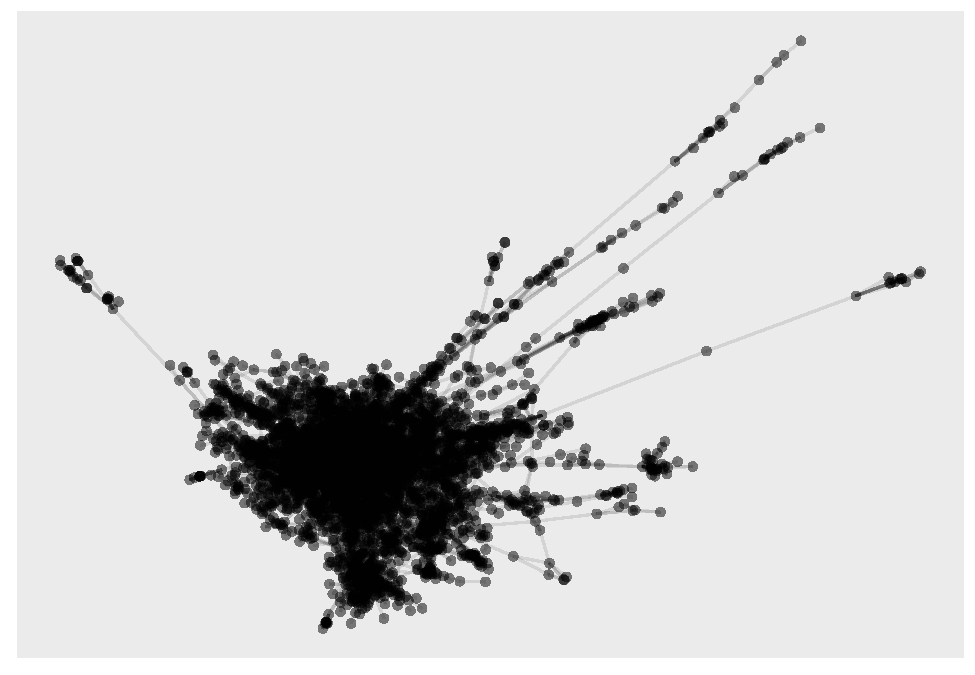
\includegraphics{_main_files/figure-latex/unnamed-chunk-113-1.pdf}

These graphs have limited use, even as exploratory data. There are some ways to mitigate against them, however:

\begin{itemize}
\item
  Consider filtering the network, as in the previous steps. Make sure you're aware of the consequences of filtering before and after you calculate network metrics, however.
\item
  For large graphs, software such as Gephi, because it gives a real-time feedback of a network visualisation, can be useful, rather than purely using a programming language such as R.
\item
  Think about whether a network diagram (or a network model at all) is the best way to represent or display your data. Could you arrive at the same conclusions with a simpler data analysis and output, such as a bar chart?
\end{itemize}

\hypertarget{other-network-visualisations}{%
\subsection{Other Network Visualisations}\label{other-network-visualisations}}

There are many other ways besides a `force-directed' graph to visualise a network.

\hypertarget{bipartite-graph}{%
\subsubsection{Bipartite graph}\label{bipartite-graph}}

Some network types are particularly suited to other visualisation methods. Bipartite networks, for example, are often visualised so that the nodes are placed in two rows, according to their types. The positions within the rows are then determined by an algorithm designed to minimise edge crossings.

\begin{Shaded}
\begin{Highlighting}[]
\NormalTok{EL }\OtherTok{=} \FunctionTok{c}\NormalTok{(}\DecValTok{1}\NormalTok{,}\DecValTok{7}\NormalTok{,}\DecValTok{2}\NormalTok{,}\DecValTok{6}\NormalTok{,}\DecValTok{3}\NormalTok{,}\DecValTok{8}\NormalTok{,}\DecValTok{2}\NormalTok{,}\DecValTok{5}\NormalTok{,}\DecValTok{4}\NormalTok{,}\DecValTok{6}\NormalTok{,}\DecValTok{1}\NormalTok{,}\DecValTok{5}\NormalTok{,}\DecValTok{2}\NormalTok{,}\DecValTok{6}\NormalTok{)}
\NormalTok{types }\OtherTok{=} \FunctionTok{rep}\NormalTok{(}\DecValTok{0}\SpecialCharTok{:}\DecValTok{1}\NormalTok{, }\AttributeTok{each=}\DecValTok{4}\NormalTok{)}
\NormalTok{g }\OtherTok{=} \FunctionTok{make\_bipartite\_graph}\NormalTok{(types, EL, }\AttributeTok{directed =} \ConstantTok{FALSE}\NormalTok{)}

\NormalTok{g }\SpecialCharTok{\%\textgreater{}\%} \FunctionTok{ggraph}\NormalTok{(}\StringTok{\textquotesingle{}bipartite\textquotesingle{}}\NormalTok{)}\SpecialCharTok{+} 
  \FunctionTok{geom\_edge\_link}\NormalTok{() }\SpecialCharTok{+} 
  \FunctionTok{geom\_node\_point}\NormalTok{(}\AttributeTok{size =} \DecValTok{10}\NormalTok{, }\FunctionTok{aes}\NormalTok{(}\AttributeTok{color =} \FunctionTok{as.character}\NormalTok{(types)))  }\SpecialCharTok{+} \FunctionTok{coord\_flip}\NormalTok{() }\SpecialCharTok{+} \FunctionTok{theme\_void}\NormalTok{() }\SpecialCharTok{+} \FunctionTok{theme}\NormalTok{(}\AttributeTok{legend.position =} \StringTok{\textquotesingle{}bottom\textquotesingle{}}\NormalTok{) }\SpecialCharTok{+} \FunctionTok{labs}\NormalTok{(}\AttributeTok{color =} \StringTok{\textquotesingle{}Type:\textquotesingle{}}\NormalTok{)}
\end{Highlighting}
\end{Shaded}

\includegraphics{_main_files/figure-latex/unnamed-chunk-114-1.pdf}

\hypertarget{adjacency-matrix}{%
\subsubsection{Adjacency Matrix}\label{adjacency-matrix}}

One popular alternative to a network diagram is an \emph{adjacency matrix.} In this case, the x and y axes contain each name in the network. A filled square is drawn for each edge, where they intersect.

This method can be particularly useful for small, dense networks.

\includegraphics{_main_files/figure-latex/unnamed-chunk-115-1.pdf}

\hypertarget{network-visualisations-with-r-and-ggraph.}{%
\section{Network Visualisations with R and ggraph.}\label{network-visualisations-with-r-and-ggraph.}}

Visualisations like the examples above can be created with another R package, called \texttt{ggraph}. This uses the same basic syntax as the plotting library \texttt{ggplot2}, we used in an earlier lesson, but adds some special functions to visualise networks.

To create a network diagram,we first create a network object as in previous lessons.

\begin{Shaded}
\begin{Highlighting}[]
\FunctionTok{library}\NormalTok{(tidygraph)}
\FunctionTok{library}\NormalTok{(tidyverse)}
\FunctionTok{library}\NormalTok{(ggraph)}
\NormalTok{letters }\OtherTok{=} \FunctionTok{read\_csv}\NormalTok{(}\StringTok{"letter\_data.csv"}\NormalTok{, }\AttributeTok{col\_types =} \FunctionTok{cols}\NormalTok{(}\AttributeTok{.default =} \StringTok{"c"}\NormalTok{))}

\NormalTok{edge\_list }\OtherTok{=}\NormalTok{ letters }\SpecialCharTok{\%\textgreater{}\%} 
  \FunctionTok{group\_by}\NormalTok{(from\_id, to\_id) }\SpecialCharTok{\%\textgreater{}\%} 
  \FunctionTok{tally}\NormalTok{(}\AttributeTok{name =} \StringTok{\textquotesingle{}weight\textquotesingle{}}\NormalTok{)}

\NormalTok{sample\_tbl\_graph }\OtherTok{=}\NormalTok{ edge\_list }\SpecialCharTok{\%\textgreater{}\%} 
  \FunctionTok{as\_tbl\_graph}\NormalTok{()}
\end{Highlighting}
\end{Shaded}

This object is then passed to the function \texttt{ggraph()}, using the pipes.

\texttt{ggraph()} tells R to begin drawing a graph. It has optional arguments: for example, you can set the layout to something other than the default using the argument \texttt{layout\ =}.

\begin{Shaded}
\begin{Highlighting}[]
\NormalTok{sample\_tbl\_graph }\SpecialCharTok{\%\textgreater{}\%} \FunctionTok{ggraph}\NormalTok{(}\AttributeTok{layout =} \StringTok{\textquotesingle{}fr\textquotesingle{}}\NormalTok{)}
\end{Highlighting}
\end{Shaded}

\includegraphics{_main_files/figure-latex/unnamed-chunk-117-1.pdf}

You'll notice that it doesn't draw anything other than a blank grey background.

\texttt{ggraph} uses the syntax as the plotting library \texttt{ggplot2}. Recall from Week 1, class 2, that plots in \texttt{ggplot2} are created by adding \texttt{geom\_} functions to the blank plot.

The same principle applies here, except with special \texttt{ggraph} geoms:

\begin{itemize}
\item
  First, \texttt{geom\_node\_point()}, will draw the nodes of your network as points. The nodes are positioned using the chosen (or default) layout algorithm.
\item
  Next, \texttt{geom\_edge\_link()} will drawn the edges as connecting lines.
\end{itemize}

\begin{Shaded}
\begin{Highlighting}[]
\NormalTok{sample\_tbl\_graph }\SpecialCharTok{\%\textgreater{}\%} 
  \FunctionTok{ggraph}\NormalTok{(}\StringTok{\textquotesingle{}fr\textquotesingle{}}\NormalTok{) }\SpecialCharTok{+} 
  \FunctionTok{geom\_node\_point}\NormalTok{() }\SpecialCharTok{+} 
  \FunctionTok{geom\_edge\_link}\NormalTok{()}
\end{Highlighting}
\end{Shaded}

\includegraphics{_main_files/figure-latex/unnamed-chunk-118-1.pdf}

There are many additional ways you can manipulate the visual appearance of your nodes and edges, for example by adding color, size, shape, arrows, and so forth.

In ggraph (and ggplot), visual elements can be manipulated in two ways: you can either specify a value for a visual property, or you can specify that a property is mapped to a particular data point.

This is all done with the relevant geom. To do the former, specify the value directly in the geom, like this:

\begin{Shaded}
\begin{Highlighting}[]
\NormalTok{sample\_tbl\_graph }\SpecialCharTok{\%\textgreater{}\%} 
  \FunctionTok{ggraph}\NormalTok{(}\StringTok{\textquotesingle{}fr\textquotesingle{}}\NormalTok{) }\SpecialCharTok{+} 
  \FunctionTok{geom\_node\_point}\NormalTok{(}\AttributeTok{size =} \DecValTok{3}\NormalTok{) }\SpecialCharTok{+} \CommentTok{\# we specified that size should be set at the value 3}
  \FunctionTok{geom\_edge\_link}\NormalTok{()}
\end{Highlighting}
\end{Shaded}

\includegraphics{_main_files/figure-latex/unnamed-chunk-119-1.pdf}

To map data to a particular data point, specify the data to be used within the geom, within a command \texttt{aes()}:

\begin{Shaded}
\begin{Highlighting}[]
\NormalTok{sample\_tbl\_graph }\SpecialCharTok{\%\textgreater{}\%} 
  \FunctionTok{mutate}\NormalTok{(}\AttributeTok{degree =} \FunctionTok{centrality\_degree}\NormalTok{()) }\SpecialCharTok{\%\textgreater{}\%} \CommentTok{\# calculate a value for degree}
  \FunctionTok{ggraph}\NormalTok{(}\StringTok{\textquotesingle{}fr\textquotesingle{}}\NormalTok{) }\SpecialCharTok{+} 
  \FunctionTok{geom\_edge\_link}\NormalTok{() }\SpecialCharTok{+} \CommentTok{\# switch around the order of the nodes and edges as it\textquotesingle{}s easier to see the node color}
  \FunctionTok{geom\_node\_point}\NormalTok{(}\AttributeTok{size =} \DecValTok{3}\NormalTok{, }\FunctionTok{aes}\NormalTok{(}\AttributeTok{color =}\NormalTok{ degree)) }\CommentTok{\# as well as the size, color is now mapped to the degree score.}
\end{Highlighting}
\end{Shaded}

\includegraphics{_main_files/figure-latex/unnamed-chunk-120-1.pdf}

Other visual properties which can be mapped or specified include \texttt{shape} and \texttt{alpha}.

The visual appearance of edges can also be adjusted, using the same syntax.

Change to a dashed line using \texttt{linetype}:

\begin{Shaded}
\begin{Highlighting}[]
\NormalTok{sample\_tbl\_graph }\SpecialCharTok{\%\textgreater{}\%} 
  \FunctionTok{mutate}\NormalTok{(}\AttributeTok{degree =} \FunctionTok{centrality\_degree}\NormalTok{()) }\SpecialCharTok{\%\textgreater{}\%} 
  \FunctionTok{ggraph}\NormalTok{(}\StringTok{\textquotesingle{}fr\textquotesingle{}}\NormalTok{) }\SpecialCharTok{+} 
  \FunctionTok{geom\_edge\_link}\NormalTok{(}\AttributeTok{linetype =} \DecValTok{5}\NormalTok{) }\SpecialCharTok{+} 
  \FunctionTok{geom\_node\_point}\NormalTok{(}\AttributeTok{size =} \DecValTok{3}\NormalTok{, }\FunctionTok{aes}\NormalTok{(}\AttributeTok{color =}\NormalTok{ degree))}
\end{Highlighting}
\end{Shaded}

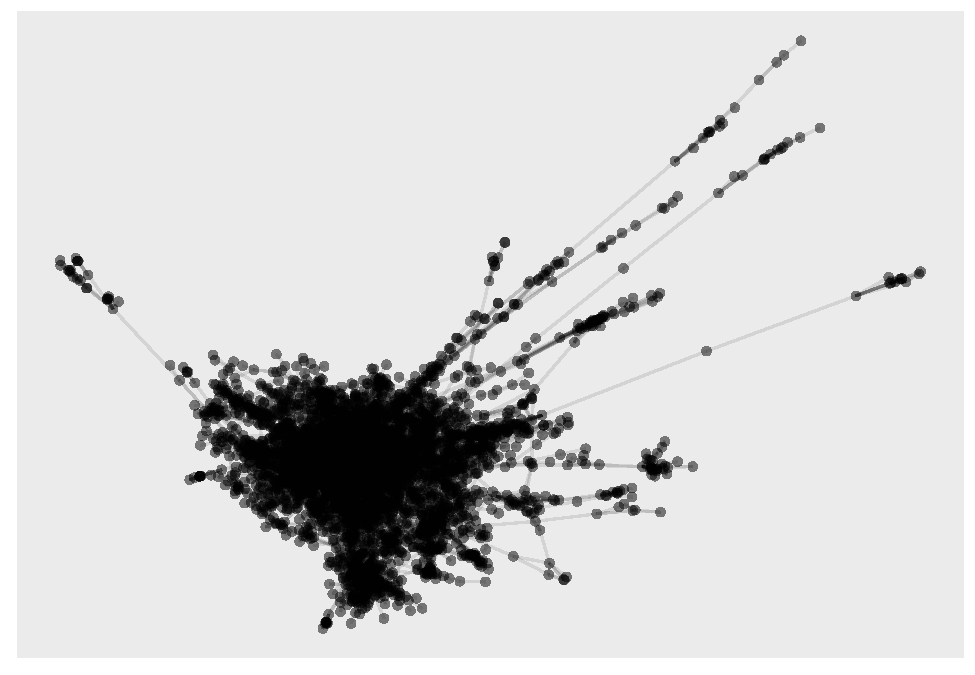
\includegraphics{_main_files/figure-latex/unnamed-chunk-121-1.pdf}

You can also add arrows, with the following syntax. The \texttt{length} and \texttt{endcap} arguments control the appearance of the arrow.

\begin{Shaded}
\begin{Highlighting}[]
\NormalTok{sample\_tbl\_graph }\SpecialCharTok{\%\textgreater{}\%} 
  \FunctionTok{mutate}\NormalTok{(}\AttributeTok{degree =} \FunctionTok{centrality\_degree}\NormalTok{()) }\SpecialCharTok{\%\textgreater{}\%} 
  \FunctionTok{ggraph}\NormalTok{(}\StringTok{\textquotesingle{}fr\textquotesingle{}}\NormalTok{) }\SpecialCharTok{+} 
  \FunctionTok{geom\_edge\_link}\NormalTok{(}\AttributeTok{linetype =} \DecValTok{5}\NormalTok{,}
                 \AttributeTok{arrow =} \FunctionTok{arrow}\NormalTok{(}\AttributeTok{length =} \FunctionTok{unit}\NormalTok{(}\DecValTok{4}\NormalTok{, }\StringTok{\textquotesingle{}mm\textquotesingle{}}\NormalTok{)), }
                   \AttributeTok{end\_cap =} \FunctionTok{circle}\NormalTok{(}\DecValTok{3}\NormalTok{, }\StringTok{\textquotesingle{}mm\textquotesingle{}}\NormalTok{)) }\SpecialCharTok{+} 
  \FunctionTok{geom\_node\_point}\NormalTok{(}\AttributeTok{size =} \DecValTok{3}\NormalTok{, }\FunctionTok{aes}\NormalTok{(}\AttributeTok{color =}\NormalTok{ degree))}
\end{Highlighting}
\end{Shaded}

\includegraphics{_main_files/figure-latex/unnamed-chunk-122-1.pdf}

\hypertarget{network-graph-layouts}{%
\subsection{Network Graph Layouts}\label{network-graph-layouts}}

Igraph has a number of graph layouts. Depending on your network size and structure, different ones may be appropriate. Where possible, it is a good idea to add some other information, for example group membership or simply node names to your visualisation, at least temporarily. That way you can check to see if the visual structures, such as clusters, centre-periphery, and orientation, make any sense. Here are the most common graph layouts:

\hypertarget{fruchterman-reingold}{%
\subsubsection{Fruchterman-Reingold}\label{fruchterman-reingold}}

\begin{Shaded}
\begin{Highlighting}[]
\NormalTok{sample\_tbl\_graph }\SpecialCharTok{\%\textgreater{}\%} 
  \FunctionTok{mutate}\NormalTok{(}\AttributeTok{degree =} \FunctionTok{centrality\_degree}\NormalTok{()) }\SpecialCharTok{\%\textgreater{}\%} 
  \FunctionTok{ggraph}\NormalTok{(}\StringTok{\textquotesingle{}fr\textquotesingle{}}\NormalTok{) }\SpecialCharTok{+} 
  \FunctionTok{geom\_edge\_link}\NormalTok{(}\AttributeTok{linetype =} \DecValTok{5}\NormalTok{,}
                 \AttributeTok{arrow =} \FunctionTok{arrow}\NormalTok{(}\AttributeTok{length =} \FunctionTok{unit}\NormalTok{(}\DecValTok{4}\NormalTok{, }\StringTok{\textquotesingle{}mm\textquotesingle{}}\NormalTok{)), }
                   \AttributeTok{end\_cap =} \FunctionTok{circle}\NormalTok{(}\DecValTok{3}\NormalTok{, }\StringTok{\textquotesingle{}mm\textquotesingle{}}\NormalTok{)) }\SpecialCharTok{+} 
  \FunctionTok{geom\_node\_point}\NormalTok{(}\AttributeTok{size =} \DecValTok{3}\NormalTok{, }\FunctionTok{aes}\NormalTok{(}\AttributeTok{color =}\NormalTok{ degree))}
\end{Highlighting}
\end{Shaded}

\includegraphics{_main_files/figure-latex/unnamed-chunk-123-1.pdf}

\hypertarget{drl}{%
\subsubsection{DRL}\label{drl}}

\begin{Shaded}
\begin{Highlighting}[]
\NormalTok{sample\_tbl\_graph }\SpecialCharTok{\%\textgreater{}\%} 
  \FunctionTok{mutate}\NormalTok{(}\AttributeTok{degree =} \FunctionTok{centrality\_degree}\NormalTok{()) }\SpecialCharTok{\%\textgreater{}\%} 
  \FunctionTok{ggraph}\NormalTok{(}\StringTok{\textquotesingle{}drl\textquotesingle{}}\NormalTok{) }\SpecialCharTok{+} 
  \FunctionTok{geom\_edge\_link}\NormalTok{(}\AttributeTok{linetype =} \DecValTok{5}\NormalTok{,}
                 \AttributeTok{arrow =} \FunctionTok{arrow}\NormalTok{(}\AttributeTok{length =} \FunctionTok{unit}\NormalTok{(}\DecValTok{4}\NormalTok{, }\StringTok{\textquotesingle{}mm\textquotesingle{}}\NormalTok{)), }
                   \AttributeTok{end\_cap =} \FunctionTok{circle}\NormalTok{(}\DecValTok{3}\NormalTok{, }\StringTok{\textquotesingle{}mm\textquotesingle{}}\NormalTok{)) }\SpecialCharTok{+} 
  \FunctionTok{geom\_node\_point}\NormalTok{(}\AttributeTok{size =} \DecValTok{3}\NormalTok{, }\FunctionTok{aes}\NormalTok{(}\AttributeTok{color =}\NormalTok{ degree))}
\end{Highlighting}
\end{Shaded}

\includegraphics{_main_files/figure-latex/unnamed-chunk-124-1.pdf}

\hypertarget{kk}{%
\subsubsection{KK}\label{kk}}

\begin{Shaded}
\begin{Highlighting}[]
\NormalTok{sample\_tbl\_graph }\SpecialCharTok{\%\textgreater{}\%} 
  \FunctionTok{mutate}\NormalTok{(}\AttributeTok{degree =} \FunctionTok{centrality\_degree}\NormalTok{()) }\SpecialCharTok{\%\textgreater{}\%} 
  \FunctionTok{ggraph}\NormalTok{(}\StringTok{\textquotesingle{}kk\textquotesingle{}}\NormalTok{) }\SpecialCharTok{+} 
  \FunctionTok{geom\_edge\_link}\NormalTok{(}\AttributeTok{linetype =} \DecValTok{5}\NormalTok{,}
                 \AttributeTok{arrow =} \FunctionTok{arrow}\NormalTok{(}\AttributeTok{length =} \FunctionTok{unit}\NormalTok{(}\DecValTok{4}\NormalTok{, }\StringTok{\textquotesingle{}mm\textquotesingle{}}\NormalTok{)), }
                   \AttributeTok{end\_cap =} \FunctionTok{circle}\NormalTok{(}\DecValTok{3}\NormalTok{, }\StringTok{\textquotesingle{}mm\textquotesingle{}}\NormalTok{)) }\SpecialCharTok{+} 
  \FunctionTok{geom\_node\_point}\NormalTok{(}\AttributeTok{size =} \DecValTok{3}\NormalTok{, }\FunctionTok{aes}\NormalTok{(}\AttributeTok{color =}\NormalTok{ degree))}
\end{Highlighting}
\end{Shaded}

\includegraphics{_main_files/figure-latex/unnamed-chunk-125-1.pdf}

\hypertarget{circle}{%
\subsubsection{Circle}\label{circle}}

\begin{Shaded}
\begin{Highlighting}[]
\NormalTok{sample\_tbl\_graph }\SpecialCharTok{\%\textgreater{}\%} 
  \FunctionTok{mutate}\NormalTok{(}\AttributeTok{degree =} \FunctionTok{centrality\_degree}\NormalTok{()) }\SpecialCharTok{\%\textgreater{}\%} 
  \FunctionTok{ggraph}\NormalTok{(}\StringTok{\textquotesingle{}circle\textquotesingle{}}\NormalTok{) }\SpecialCharTok{+} 
  \FunctionTok{geom\_edge\_link}\NormalTok{(}\AttributeTok{linetype =} \DecValTok{5}\NormalTok{,}
                 \AttributeTok{arrow =} \FunctionTok{arrow}\NormalTok{(}\AttributeTok{length =} \FunctionTok{unit}\NormalTok{(}\DecValTok{4}\NormalTok{, }\StringTok{\textquotesingle{}mm\textquotesingle{}}\NormalTok{)), }
                   \AttributeTok{end\_cap =} \FunctionTok{circle}\NormalTok{(}\DecValTok{3}\NormalTok{, }\StringTok{\textquotesingle{}mm\textquotesingle{}}\NormalTok{)) }\SpecialCharTok{+} 
  \FunctionTok{geom\_node\_point}\NormalTok{(}\AttributeTok{size =} \DecValTok{3}\NormalTok{, }\FunctionTok{aes}\NormalTok{(}\AttributeTok{color =}\NormalTok{ degree))}
\end{Highlighting}
\end{Shaded}

\includegraphics{_main_files/figure-latex/unnamed-chunk-126-1.pdf}

\hypertarget{edge-types}{%
\subsubsection{Edge types}\label{edge-types}}

You can also make extenstive changes to the type of edge. In many cases, these may make the diagram more readable. Some have particular uses, for example \texttt{geom\_edge\_fan()} is used for a multigraph (where you have multiple different types of edges), and \texttt{geom\_edge\_arc} can be useful for when you want to visualise the difference between incoming and outgoing edges:

\begin{Shaded}
\begin{Highlighting}[]
\NormalTok{sample\_tbl\_graph }\SpecialCharTok{\%\textgreater{}\%} 
  \FunctionTok{mutate}\NormalTok{(}\AttributeTok{degree =} \FunctionTok{centrality\_degree}\NormalTok{()) }\SpecialCharTok{\%\textgreater{}\%} 
  \FunctionTok{ggraph}\NormalTok{(}\StringTok{\textquotesingle{}fr\textquotesingle{}}\NormalTok{) }\SpecialCharTok{+} 
  \FunctionTok{geom\_edge\_bend}\NormalTok{(}\AttributeTok{linetype =} \DecValTok{5}\NormalTok{,}
                 \AttributeTok{arrow =} \FunctionTok{arrow}\NormalTok{(}\AttributeTok{length =} \FunctionTok{unit}\NormalTok{(}\DecValTok{4}\NormalTok{, }\StringTok{\textquotesingle{}mm\textquotesingle{}}\NormalTok{)), }
                   \AttributeTok{end\_cap =} \FunctionTok{circle}\NormalTok{(}\DecValTok{3}\NormalTok{, }\StringTok{\textquotesingle{}mm\textquotesingle{}}\NormalTok{)) }\SpecialCharTok{+} 
  \FunctionTok{geom\_node\_point}\NormalTok{(}\AttributeTok{size =} \DecValTok{3}\NormalTok{, }\FunctionTok{aes}\NormalTok{(}\AttributeTok{color =}\NormalTok{ degree))}
\end{Highlighting}
\end{Shaded}

\includegraphics{_main_files/figure-latex/unnamed-chunk-127-1.pdf}

\begin{Shaded}
\begin{Highlighting}[]
\NormalTok{sample\_tbl\_graph }\SpecialCharTok{\%\textgreater{}\%} 
  \FunctionTok{mutate}\NormalTok{(}\AttributeTok{degree =} \FunctionTok{centrality\_degree}\NormalTok{()) }\SpecialCharTok{\%\textgreater{}\%} 
  \FunctionTok{ggraph}\NormalTok{(}\StringTok{\textquotesingle{}fr\textquotesingle{}}\NormalTok{) }\SpecialCharTok{+} 
  \FunctionTok{geom\_edge\_arc}\NormalTok{(}\AttributeTok{linetype =} \DecValTok{5}\NormalTok{,}
                 \AttributeTok{arrow =} \FunctionTok{arrow}\NormalTok{(}\AttributeTok{length =} \FunctionTok{unit}\NormalTok{(}\DecValTok{4}\NormalTok{, }\StringTok{\textquotesingle{}mm\textquotesingle{}}\NormalTok{)), }
                   \AttributeTok{end\_cap =} \FunctionTok{circle}\NormalTok{(}\DecValTok{3}\NormalTok{, }\StringTok{\textquotesingle{}mm\textquotesingle{}}\NormalTok{)) }\SpecialCharTok{+} 
  \FunctionTok{geom\_node\_point}\NormalTok{(}\AttributeTok{size =} \DecValTok{3}\NormalTok{, }\FunctionTok{aes}\NormalTok{(}\AttributeTok{color =}\NormalTok{ degree))}
\end{Highlighting}
\end{Shaded}

\includegraphics{_main_files/figure-latex/unnamed-chunk-128-1.pdf}

\hypertarget{tree}{%
\subsubsection{Tree}\label{tree}}

\begin{Shaded}
\begin{Highlighting}[]
\NormalTok{sample\_tbl\_graph }\SpecialCharTok{\%\textgreater{}\%} 
  \FunctionTok{mutate}\NormalTok{(}\AttributeTok{degree =} \FunctionTok{centrality\_degree}\NormalTok{()) }\SpecialCharTok{\%\textgreater{}\%} 
  \FunctionTok{ggraph}\NormalTok{(}\StringTok{\textquotesingle{}tree\textquotesingle{}}\NormalTok{) }\SpecialCharTok{+} 
  \FunctionTok{geom\_edge\_bend}\NormalTok{(}\AttributeTok{linetype =} \DecValTok{5}\NormalTok{,}
                 \AttributeTok{arrow =} \FunctionTok{arrow}\NormalTok{(}\AttributeTok{length =} \FunctionTok{unit}\NormalTok{(}\DecValTok{4}\NormalTok{, }\StringTok{\textquotesingle{}mm\textquotesingle{}}\NormalTok{)), }
                   \AttributeTok{end\_cap =} \FunctionTok{circle}\NormalTok{(}\DecValTok{3}\NormalTok{, }\StringTok{\textquotesingle{}mm\textquotesingle{}}\NormalTok{)) }\SpecialCharTok{+} 
  \FunctionTok{geom\_node\_point}\NormalTok{(}\AttributeTok{size =} \DecValTok{3}\NormalTok{, }\FunctionTok{aes}\NormalTok{(}\AttributeTok{color =}\NormalTok{ degree))}
\end{Highlighting}
\end{Shaded}

\includegraphics{_main_files/figure-latex/unnamed-chunk-129-1.pdf}

\hypertarget{bipartite}{%
\subsubsection{Bipartite}\label{bipartite}}

It is worth checking some of these out, particularly if you have a specific network structure, for example a hierarchy, or if you have a bipartite network.

Also note there are lots of other ways to visualise a network, for example by making a heatmap from an adjacency matrix. It's worth experimenting a bit with these (and explaining choices in your final project).

\hypertarget{ggraph-and-other-tidyverse-functions}{%
\subsection{Ggraph and other tidyverse functions}\label{ggraph-and-other-tidyverse-functions}}

You can use the dplyr pipes to perform calculations, filter the data and then visualise it, all in one go:

\begin{Shaded}
\begin{Highlighting}[]
\NormalTok{sample\_tbl\_graph }\SpecialCharTok{\%\textgreater{}\%} 
  \FunctionTok{activate}\NormalTok{(nodes)}\SpecialCharTok{\%\textgreater{}\%} 
  \FunctionTok{mutate}\NormalTok{(}\AttributeTok{degree =} \FunctionTok{centrality\_degree}\NormalTok{(}\AttributeTok{mode =} \StringTok{\textquotesingle{}total\textquotesingle{}}\NormalTok{)) }\SpecialCharTok{\%\textgreater{}\%} \CommentTok{\# calculate total degree }
  \FunctionTok{filter}\NormalTok{(degree }\SpecialCharTok{\textgreater{}}\DecValTok{2}\NormalTok{) }\SpecialCharTok{\%\textgreater{}\%} \CommentTok{\# filter to only include nodes with a degree greater than 2.}
  \FunctionTok{ggraph}\NormalTok{(}\StringTok{\textquotesingle{}fr\textquotesingle{}}\NormalTok{) }\SpecialCharTok{+} 
  \FunctionTok{geom\_node\_point}\NormalTok{() }\SpecialCharTok{+} 
  \FunctionTok{geom\_edge\_link}\NormalTok{()}
\end{Highlighting}
\end{Shaded}

\includegraphics{_main_files/figure-latex/unnamed-chunk-130-1.pdf}

\hypertarget{add-node-labels}{%
\subsection{Add node labels}\label{add-node-labels}}

Add \texttt{geom\_node\_text()} to add text labels to your network. In a larger network, it can be helpful to only show labels belonging to the most-connected nodes.

To do this, join the people table to the nodes table, then use ggraph, setting the \texttt{label} aesthetic. Another \texttt{dplyr} verb, \texttt{if\_else} allows you to add conditions to the label command.

Here, I've used if\_else to return the label if the node's degree score is more than 10:

A the moment, we only have the IDs for each node. In a further step we can join back the actual names and use these as labels.

\begin{Shaded}
\begin{Highlighting}[]
\NormalTok{sample\_tbl\_graph }\SpecialCharTok{\%\textgreater{}\%} 
  \FunctionTok{activate}\NormalTok{(nodes) }\SpecialCharTok{\%\textgreater{}\%} 
  \FunctionTok{mutate}\NormalTok{(}\AttributeTok{degree =} \FunctionTok{centrality\_degree}\NormalTok{(}\AttributeTok{mode =} \StringTok{\textquotesingle{}total\textquotesingle{}}\NormalTok{))  }\SpecialCharTok{\%\textgreater{}\%} 
  \FunctionTok{ggraph}\NormalTok{(}\StringTok{\textquotesingle{}nicely\textquotesingle{}}\NormalTok{) }\SpecialCharTok{+} 
  \FunctionTok{geom\_node\_point}\NormalTok{(}\FunctionTok{aes}\NormalTok{(}\AttributeTok{size =}\NormalTok{ degree)) }\SpecialCharTok{+} 
  \FunctionTok{geom\_node\_text}\NormalTok{(}\FunctionTok{aes}\NormalTok{(}\AttributeTok{label =} \FunctionTok{if\_else}\NormalTok{(degree }\SpecialCharTok{\textgreater{}}\DecValTok{10}\NormalTok{, name, }\ConstantTok{NULL}\NormalTok{), }\AttributeTok{size =}\NormalTok{ degree), }\AttributeTok{repel =} \ConstantTok{TRUE}\NormalTok{) }\SpecialCharTok{+} 
  \FunctionTok{geom\_edge\_link}\NormalTok{(}\AttributeTok{alpha =}\NormalTok{ .}\DecValTok{2}\NormalTok{)}
\end{Highlighting}
\end{Shaded}

\begin{verbatim}
## Warning: Removed 240 rows containing missing values (geom_text_repel).
\end{verbatim}

\includegraphics{_main_files/figure-latex/unnamed-chunk-131-1.pdf}

\hypertarget{calculating-and-coloring-by-community-detection}{%
\subsection{Calculating and coloring by community detection}\label{calculating-and-coloring-by-community-detection}}

One very common visualisation is colouring the various groups in the network, which might give us a clue as to its structure.

\begin{Shaded}
\begin{Highlighting}[]
\NormalTok{sample\_tbl\_graph }\SpecialCharTok{\%\textgreater{}\%} 
  \FunctionTok{as.undirected}\NormalTok{() }\SpecialCharTok{\%\textgreater{}\%} 
  \FunctionTok{as\_tbl\_graph}\NormalTok{() }\SpecialCharTok{\%\textgreater{}\%} 
  \FunctionTok{activate}\NormalTok{(nodes) }\SpecialCharTok{\%\textgreater{}\%} 
  \FunctionTok{mutate}\NormalTok{(}\AttributeTok{degree =} \FunctionTok{centrality\_degree}\NormalTok{(}\AttributeTok{mode =} \StringTok{\textquotesingle{}total\textquotesingle{}}\NormalTok{))  }\SpecialCharTok{\%\textgreater{}\%} 
  \FunctionTok{mutate}\NormalTok{(}\AttributeTok{community =} \FunctionTok{group\_edge\_betweenness}\NormalTok{(}\AttributeTok{weights =}\ConstantTok{NULL}\NormalTok{)) }\SpecialCharTok{\%\textgreater{}\%} 
  \FunctionTok{filter}\NormalTok{(community }\SpecialCharTok{\%in\%} \DecValTok{1}\SpecialCharTok{:}\DecValTok{4}\NormalTok{) }\SpecialCharTok{\%\textgreater{}\%} 
  \FunctionTok{ggraph}\NormalTok{(}\StringTok{\textquotesingle{}nicely\textquotesingle{}}\NormalTok{) }\SpecialCharTok{+} 
  \FunctionTok{geom\_node\_point}\NormalTok{(}\FunctionTok{aes}\NormalTok{(}\AttributeTok{size =}\NormalTok{ degree, }\AttributeTok{color =} \FunctionTok{as.character}\NormalTok{(community))) }\SpecialCharTok{+} 
  \FunctionTok{geom\_edge\_link}\NormalTok{(}\AttributeTok{alpha =}\NormalTok{ .}\DecValTok{2}\NormalTok{)}
\end{Highlighting}
\end{Shaded}

\begin{verbatim}
## Warning in cluster_edge_betweenness(graph = .G(), weights = weights, directed =
## directed): At core/community/edge_betweenness.c:485 : Membership vector will be
## selected based on the lowest modularity score.
\end{verbatim}

\begin{verbatim}
## Warning in cluster_edge_betweenness(graph = .G(), weights = weights, directed
## = directed): At core/community/edge_betweenness.c:492 : Modularity calculation
## with weighted edge betweenness community detection might not make sense --
## modularity treats edge weights as similarities while edge betwenness treats them
## as distances.
\end{verbatim}

\includegraphics{_main_files/figure-latex/unnamed-chunk-132-1.pdf}

\hypertarget{what-makes-a-good-network-visualisation}{%
\section{What makes a good network visualisation?}\label{what-makes-a-good-network-visualisation}}

You will rarely be able to make a good network visualisation simply by pushing a button and using the default settings. You should think about what your network is trying to communicate and to what audience, and spend some time

\begin{itemize}
\item
  Treat the diagram as carefully as you would an essay or other piece of text. Is it easy to understand?
\item
  Make sure you really need a network graph, and that another method of communicating the information wouldn't be better. For example, if your diagram is simply showing the most influential nodes, would a bar chart (or even a table) with their degree work just as well?
\item
  Use colour/shape/size if you need to, but make sure you explain what each element is doing.
\item
  Spend some time showing your readers how to `read' the visualisation. What is interesting about the left/right/top/bottom of the diagram? What is the significance of nodes grouped together, and what about nodes in the centre versus nodes towards the edge? Are there obvious clusters and gaps, and do these show up in the visualisation?
\end{itemize}

\hypertarget{case-study-scientists-and-politicians}{%
\section{Case study: Scientists and Politicians}\label{case-study-scientists-and-politicians}}

In this final section, I'll demonstrate how these methods might be used to carry out exploratory data analysis on the sample letter dataset.

The node attributes can used either to filter the network, or added as extra visual elements. Doing so helps us to understand a bit more about why the network might look the way it does.

First, load the same node attributes table as before:

\begin{Shaded}
\begin{Highlighting}[]
\NormalTok{node\_attributes }\OtherTok{=} \FunctionTok{read\_csv}\NormalTok{(}\StringTok{\textquotesingle{}node\_attributes.csv\textquotesingle{}}\NormalTok{)}
\end{Highlighting}
\end{Shaded}

\begin{verbatim}
## Rows: 248 Columns: 13
## -- Column specification --------------------------------------------------------
## Delimiter: ","
## chr (11): name, main_name, all_names, links, gender, roles_titles, wikidata_...
## dbl  (2): birth_year, death_year
## 
## i Use `spec()` to retrieve the full column specification for this data.
## i Specify the column types or set `show_col_types = FALSE` to quiet this message.
\end{verbatim}

This external information might help us to make sense of the clusters found by the community detection algorithm used above. One of the fields in the data is whether that person is listed as a politician on Wikidata: the field is a simple flag of either \texttt{yes} or \texttt{no}.

To check whether this might be a clue towards the structure of the network, we will set the \emph{color} to the community detection results, and the \emph{shape} to the politician flag, with the following code:

\begin{Shaded}
\begin{Highlighting}[]
\NormalTok{sample\_tbl\_graph }\SpecialCharTok{\%\textgreater{}\%} 
  \FunctionTok{as.undirected}\NormalTok{() }\SpecialCharTok{\%\textgreater{}\%} 
  \FunctionTok{as\_tbl\_graph}\NormalTok{()}\SpecialCharTok{\%\textgreater{}\%} 
  \FunctionTok{activate}\NormalTok{(nodes) }\SpecialCharTok{\%\textgreater{}\%} 
  \FunctionTok{mutate}\NormalTok{(}\AttributeTok{degree =} \FunctionTok{centrality\_degree}\NormalTok{(}\AttributeTok{mode =} \StringTok{\textquotesingle{}total\textquotesingle{}}\NormalTok{)) }\SpecialCharTok{\%\textgreater{}\%} 
  \FunctionTok{left\_join}\NormalTok{(node\_attributes) }\SpecialCharTok{\%\textgreater{}\%} 
  \FunctionTok{mutate}\NormalTok{(}\AttributeTok{community =} \FunctionTok{group\_edge\_betweenness}\NormalTok{(}\AttributeTok{weights =}\ConstantTok{NULL}\NormalTok{)) }\SpecialCharTok{\%\textgreater{}\%} 
  \FunctionTok{filter}\NormalTok{(community }\SpecialCharTok{\%in\%} \DecValTok{1}\SpecialCharTok{:}\DecValTok{4}\NormalTok{) }\SpecialCharTok{\%\textgreater{}\%} 
  \FunctionTok{ggraph}\NormalTok{(}\StringTok{\textquotesingle{}fr\textquotesingle{}}\NormalTok{) }\SpecialCharTok{+} 
  \FunctionTok{geom\_edge\_link}\NormalTok{(}\AttributeTok{alpha =}\NormalTok{ .}\DecValTok{2}\NormalTok{)}\SpecialCharTok{+} 
  \FunctionTok{geom\_node\_point}\NormalTok{(}\FunctionTok{aes}\NormalTok{(}\AttributeTok{size =}\NormalTok{ degree, }\AttributeTok{color =} \FunctionTok{as.character}\NormalTok{(community), }\AttributeTok{shape =}\NormalTok{ politician))  }\SpecialCharTok{+} 
  \FunctionTok{geom\_node\_text}\NormalTok{(}\FunctionTok{aes}\NormalTok{(}\AttributeTok{label =} \FunctionTok{ifelse}\NormalTok{(degree }\SpecialCharTok{\textgreater{}}\DecValTok{2}\NormalTok{, main\_name, }\ConstantTok{NA}\NormalTok{)), }\AttributeTok{size =} \FloatTok{2.5}\NormalTok{, }\AttributeTok{repel =}\NormalTok{ T) }\SpecialCharTok{+} 
  \FunctionTok{theme}\NormalTok{(}\AttributeTok{legend.position =} \StringTok{\textquotesingle{}none\textquotesingle{}}\NormalTok{)}
\end{Highlighting}
\end{Shaded}

\includegraphics{_main_files/figure-latex/unnamed-chunk-134-1.pdf}

It does look like one of the four clusters (cluster 2) has far fewer politicians. This cluster seems to be a group of what might be described as natural philosophers.

Other things to look out for in this visualisation:

\begin{itemize}
\item
  What is the importance of the nodes sitting in between the scientists and the politicians? What metrics might they score highly on, and what role might they occupy in this system? What kinds of information may they be able to pass on?
\item
  What is the position of Athanasius Kircher? What does it mean to be on the periphery of this network?
\item
  What effect might additional data have on the metrics in this network? Should this make us cautious about any inference from this network?
\end{itemize}

\hypertarget{conclusions-1}{%
\section{Conclusions}\label{conclusions-1}}

Hopefully, from reading this chapter, you'll be convinced that network visualisations are useful, but that they should also be approached with caution. The bottom line is, visualisations of themselves are not a result: at the very least, they need extensive commentary in order to explain them, and in some cases, they may simply be useful ways of describing the network.

At the same time, in combination with the additional attributes from our data model, thoughtful visualisations can be incredibly useful for exploring a network dataset, revealing patterns that are otherwise hidden. I encourage you to use visualisations in your final project if they make sense, are not just `hairballs', and if they can be justified with relevant commentary.

\hypertarget{week-5-class-2-other-network-types}{%
\chapter{Week 5, class 2: Other network types}\label{week-5-class-2-other-network-types}}

\hypertarget{ego-networks}{%
\section{Ego Networks}\label{ego-networks}}

Very often when applying network analysis to humanities datasets, you'll be working with \emph{ego networks}. An ego network is a network seen from the perspective of a focal node, known as the ego, and all the nodes to which it is connected, known as \emph{alters}. In a true ego network, the network will include all the links \emph{between} the alters.

\begin{figure}

{\centering \includegraphics{_main_files/figure-latex/unnamed-chunk-135-1} 

}

\caption{Example ego network}\label{fig:unnamed-chunk-135}
\end{figure}

These types of networks are very common in real-world networks because data is often collected from the perspective of an ego node or a number of ego nodes, for example, in a survey, or perhaps in a collection of correspondence. Because of this it is important to understand what they are, and think about whether the data is representative.

At the same time, ego network data can be very useful. Studies have shown that many metrics in an ego network correlate strongly with metrics from a full network (meaning that if an alter is central to the ego network, it is likely also central if we had the full network data too.

Network analysis from the point of view of egos can tell us about the structure of a particular node and its relationship to its neighbours. Comparing many ego networks can be used to good effect. \href{https://www.pnas.org/doi/10.1073/pnas.2206070119}{Lerman et al (2022)} created a list of features (attributes) for the citation ego networks of authors elected to the National Academy of Sciences, successfully using those features to predict the gender of the author:

\begin{quote}
Women's ego networks have higher average degree, edge density, and clustering coefficient. Together, these features suggest that women are more tightly embedded within their research communities. This is consistent with previous findings that women tend to gravitate to certain communities (\href{https://www.pnas.org/doi/10.1073/pnas.2206070119\#core-r11}{11}). Women have fewer peers than men, but these peers are more productive (publish more papers) and receive more citations. Finally, women NAS members have more women among their peers.
\end{quote}

Many of the datasets you might be considering using for your final project may in fact be ego networks. It is worth thinking about the implications of this, and considering which kinds of metrics, or comparisons would work best. Is each ego network collected using the same method? If not, does this skew the results?

\hypertarget{case-study-a-spotify-ego-network}{%
\section{Case Study: A Spotify Ego Network}\label{case-study-a-spotify-ego-network}}

This section walks through the code for creating and analysing an ego network drawn from a very different type of humanities dataset: Spotify's `related' artists information. This is available through Spotify's API. One function of the API lets us download the twenty `most-related' artists to a given `seed' artist. The algorithm for how the most-related are calculated is not public, but it's likely by comparing overlapping listeners (if lots of people listen to both artist X and artist Y, those artists are marked as related).

\hypertarget{requirements}{%
\subsubsection{Requirements}\label{requirements}}

If you want to complete the (optional) exercise in the corresponding file on CSC notebooks, you'll need to sign up for a Spotify developer account. Once you've done this, create a new application using the dashboard. This will give you the necessary client ID and password. You'll then need to install the \texttt{spotifyr} package using \texttt{install.packages(\textquotesingle{}spotifyr)}.

An exercise relating to the bipartite network below is another option - if for whatever reason you don't want to sign up for an account, or have difficulty accessing the API. The data for this is already available.

\hypertarget{get-related-artists-from-the-spotify-api.}{%
\subsubsection{Get related artists from the Spotify API.}\label{get-related-artists-from-the-spotify-api.}}

The \texttt{spotifyr} package makes it easy to access the Spotify API functions using R.

Once you have installed the spotifyr package, you need to tell it where to find your user ID and password. Copy these from your dashboard on the Spotify API page. Then, use the following code to temporarily store them in R's memory:

\begin{Shaded}
\begin{Highlighting}[]
 \CommentTok{\#Sys.setenv(SPOTIFY\_CLIENT\_ID = \textquotesingle{}\textquotesingle{}) \# uncomment these lines and add your client ID and password here, in between the quotation marks. }
 \CommentTok{\#Sys.setenv(SPOTIFY\_CLIENT\_SECRET = \textquotesingle{}\textquotesingle{})}
\end{Highlighting}
\end{Shaded}

Next, you'll use the command \texttt{get\_spotify\_access\_token()} to use this ID and password to generate an access token.

Following this, we need to find the spotify ID for the `ego' artist. The easiest way to do this is with the \texttt{get\_artist\_audio\_features()} function. This can take a character string and will return the closest match, if an ID is not specified. To get the ID for the band Radiohead, we do the following:

\begin{Shaded}
\begin{Highlighting}[]
\CommentTok{\# install.packages(\textquotesingle{}spotifyr\textquotesingle{}) \# install the package if necessary}

\FunctionTok{library}\NormalTok{(spotifyr)}


\NormalTok{access\_token }\OtherTok{\textless{}{-}} \FunctionTok{get\_spotify\_access\_token}\NormalTok{()}


\NormalTok{radiohead }\OtherTok{\textless{}{-}} \FunctionTok{get\_artist\_audio\_features}\NormalTok{(}\StringTok{\textquotesingle{}radiohead\textquotesingle{}}\NormalTok{)}

\FunctionTok{glimpse}\NormalTok{(radiohead)}
\end{Highlighting}
\end{Shaded}

\begin{verbatim}
## Rows: 193
## Columns: 39
## $ artist_name                  <chr> "Radiohead", "Radiohead", "Radiohead", "R~
## $ artist_id                    <chr> "4Z8W4fKeB5YxbusRsdQVPb", "4Z8W4fKeB5Yxbu~
## $ album_id                     <chr> "6ofEQubaL265rIW6WnCU8y", "6ofEQubaL265rI~
## $ album_type                   <chr> "album", "album", "album", "album", "albu~
## $ album_images                 <list> [<data.frame[3 x 3]>], [<data.frame[3 x ~
## $ album_release_date           <chr> "2021-11-05", "2021-11-05", "2021-11-05",~
## $ album_release_year           <dbl> 2021, 2021, 2021, 2021, 2021, 2021, 2021,~
## $ album_release_date_precision <chr> "day", "day", "day", "day", "day", "day",~
## $ danceability                 <dbl> 0.296, 0.630, 0.488, 0.167, 0.165, 0.402,~
## $ energy                       <dbl> 0.463, 0.428, 0.754, 0.302, 0.146, 0.757,~
## $ key                          <int> 5, 5, 2, 6, 6, 7, 0, 3, 2, 7, 7, 0, 11, 1~
## $ loudness                     <dbl> -11.412, -15.520, -8.552, -11.644, -21.35~
## $ mode                         <int> 0, 1, 1, 0, 1, 0, 1, 1, 1, 1, 1, 1, 0, 0,~
## $ speechiness                  <dbl> 0.0449, 0.0358, 0.0378, 0.0345, 0.0362, 0~
## $ acousticness                 <dbl> 7.05e-01, 2.62e-01, 2.37e-03, 3.16e-01, 8~
## $ instrumentalness             <dbl> 4.82e-02, 8.52e-01, 8.51e-01, 7.97e-01, 8~
## $ liveness                     <dbl> 0.0954, 0.2780, 0.2240, 0.1100, 0.1090, 0~
## $ valence                      <dbl> 0.0629, 0.1590, 0.3880, 0.1900, 0.0577, 0~
## $ tempo                        <dbl> 123.943, 112.923, 91.517, 102.026, 134.50~
## $ track_id                     <chr> "62dUmjtkYOUwYOALt6pefh", "797AyTQcqoQgqW~
## $ analysis_url                 <chr> "https://api.spotify.com/v1/audio-analysi~
## $ time_signature               <int> 5, 4, 4, 4, 3, 4, 4, 3, 5, 4, 3, 4, 4, 4,~
## $ artists                      <list> [<data.frame[1 x 6]>], [<data.frame[1 x ~
## $ available_markets            <list> <"AD", "AE", "AG", "AL", "AM", "AO", "AR~
## $ disc_number                  <int> 1, 1, 1, 1, 1, 1, 1, 1, 1, 1, 1, 2, 2, 2,~
## $ duration_ms                  <int> 251426, 284506, 351693, 356333, 222600, 3~
## $ explicit                     <lgl> FALSE, FALSE, FALSE, FALSE, FALSE, FALSE,~
## $ track_href                   <chr> "https://api.spotify.com/v1/tracks/62dUmj~
## $ is_local                     <lgl> FALSE, FALSE, FALSE, FALSE, FALSE, FALSE,~
## $ track_name                   <chr> "Everything In Its Right Place", "Kid A",~
## $ track_preview_url            <chr> "https://p.scdn.co/mp3-preview/74e765ad68~
## $ track_number                 <int> 1, 2, 3, 4, 5, 6, 7, 8, 9, 10, 11, 1, 2, ~
## $ type                         <chr> "track", "track", "track", "track", "trac~
## $ track_uri                    <chr> "spotify:track:62dUmjtkYOUwYOALt6pefh", "~
## $ external_urls.spotify        <chr> "https://open.spotify.com/track/62dUmjtkY~
## $ album_name                   <chr> "KID A MNESIA", "KID A MNESIA", "KID A MN~
## $ key_name                     <chr> "F", "F", "D", "F#", "F#", "G", "C", "D#"~
## $ mode_name                    <chr> "minor", "major", "major", "minor", "majo~
## $ key_mode                     <chr> "F minor", "F major", "D major", "F# mino~
\end{verbatim}

This returns all of Radiohead's tracks along with some more information. The second column in each row is the \texttt{artist\_id}, in this case \texttt{4Z8W4fKeB5YxbusRsdQVPb}, which we will use as the input for further functions.

The function to get the related artists to one artist is \texttt{get\_related\_artists()}. The below syntax will get Radiohead's related artists list:

\begin{Shaded}
\begin{Highlighting}[]
\NormalTok{radiohead\_related }\OtherTok{=}\NormalTok{ spotifyr}\SpecialCharTok{::}\FunctionTok{get\_related\_artists}\NormalTok{(}\StringTok{\textquotesingle{}4Z8W4fKeB5YxbusRsdQVPb\textquotesingle{}}\NormalTok{)}

\FunctionTok{glimpse}\NormalTok{(radiohead\_related)}
\end{Highlighting}
\end{Shaded}

\begin{verbatim}
## Rows: 20
## Columns: 11
## $ genres                <list> <"art pop", "electronica", "glitch pop", "indie~
## $ href                  <chr> "https://api.spotify.com/v1/artists/4CvTDPKA6W06~
## $ id                    <chr> "4CvTDPKA6W06DRfBnZKrau", "7MhMgCo0Bl0Kukl93PZbY~
## $ images                <list> [<data.frame[3 x 3]>], [<data.frame[3 x 3]>], [~
## $ name                  <chr> "Thom Yorke", "Blur", "Pixies", "Portishead", "J~
## $ popularity            <int> 58, 69, 72, 61, 61, 60, 58, 59, 59, 56, 64, 64, ~
## $ type                  <chr> "artist", "artist", "artist", "artist", "artist"~
## $ uri                   <chr> "spotify:artist:4CvTDPKA6W06DRfBnZKrau", "spotif~
## $ external_urls.spotify <chr> "https://open.spotify.com/artist/4CvTDPKA6W06DRf~
## $ followers.href        <lgl> NA, NA, NA, NA, NA, NA, NA, NA, NA, NA, NA, NA, ~
## $ followers.total       <int> 863865, 2631056, 2315315, 1645710, 901898, 76871~
\end{verbatim}

The result is a dataframe with a list of the 20 closest-related artists to Radiohead, using Spotify's algorithm, with some more information including the artists' popularity and genres - and their Spotify ID. This can be visualised using the method from the previous lesson:

\begin{Shaded}
\begin{Highlighting}[]
\FunctionTok{library}\NormalTok{(ggraph)}
\FunctionTok{library}\NormalTok{(tidygraph)}
\FunctionTok{library}\NormalTok{(igraph)}
\NormalTok{radiohead\_related }\SpecialCharTok{\%\textgreater{}\%} 
  \FunctionTok{mutate}\NormalTok{(}\AttributeTok{ego\_name =} \StringTok{\textquotesingle{}Radiohead\textquotesingle{}}\NormalTok{) }\SpecialCharTok{\%\textgreater{}\%} 
  \FunctionTok{distinct}\NormalTok{( ego\_name, name) }\SpecialCharTok{\%\textgreater{}\%} 
  \FunctionTok{as\_tbl\_graph}\NormalTok{() }\SpecialCharTok{\%\textgreater{}\%} 
  \FunctionTok{ggraph}\NormalTok{(}\StringTok{\textquotesingle{}stress\textquotesingle{}}\NormalTok{) }\SpecialCharTok{+} \FunctionTok{geom\_edge\_link}\NormalTok{() }\SpecialCharTok{+} 
  \FunctionTok{geom\_node\_point}\NormalTok{(}\AttributeTok{size =} \DecValTok{20}\NormalTok{, }\AttributeTok{fill =} \StringTok{\textquotesingle{}white\textquotesingle{}}\NormalTok{, }\AttributeTok{color =} \StringTok{\textquotesingle{}black\textquotesingle{}}\NormalTok{, }\AttributeTok{pch =} \DecValTok{21}\NormalTok{)}\SpecialCharTok{+} 
  \FunctionTok{geom\_node\_text}\NormalTok{(}\AttributeTok{size =} \DecValTok{3}\NormalTok{, }\FunctionTok{aes}\NormalTok{(}\AttributeTok{label =}\NormalTok{name))}
\end{Highlighting}
\end{Shaded}

\includegraphics{_main_files/figure-latex/unnamed-chunk-139-1.pdf}

\hypertarget{crawling-through-the-related-artists-information}{%
\subsubsection{`Crawling' through the related artists information}\label{crawling-through-the-related-artists-information}}

As you might be able to tell, there is very little useful information in this type of ego network: which only includes links to and from the ego node. Each `alter' has a degree of one, and will have the same scores for all network metrics.

However, we can use the new artists' IDs to `crawl' through the API and get the 20 most related artists for each of them, taking a \href{https://en.wikipedia.org/wiki/Snowball_sampling}{snowball sample} approach to creating a network. The easiest way to do this is to use a R function \texttt{lapply}, which applies a function to every element in a list, and returns a new list.

\begin{Shaded}
\begin{Highlighting}[]
\NormalTok{radiohead\_related\_related }\OtherTok{=} \FunctionTok{lapply}\NormalTok{(radiohead\_related}\SpecialCharTok{$}\NormalTok{id, get\_related\_artists)}

\NormalTok{radiohead\_related\_related }\OtherTok{=}\NormalTok{ data.table}\SpecialCharTok{::}\FunctionTok{rbindlist}\NormalTok{(radiohead\_related\_related)}

\NormalTok{radiohead\_related\_related }\OtherTok{=}\NormalTok{ radiohead\_related\_related }\SpecialCharTok{\%\textgreater{}\%} 
  \FunctionTok{mutate}\NormalTok{(}\AttributeTok{seed\_id =} \FunctionTok{rep}\NormalTok{(radiohead\_related}\SpecialCharTok{$}\NormalTok{id, }\AttributeTok{each=} \DecValTok{20}\NormalTok{))}\SpecialCharTok{\%\textgreater{}\%} 
  \FunctionTok{mutate}\NormalTok{(}\AttributeTok{ego\_name =} \FunctionTok{rep}\NormalTok{(radiohead\_related}\SpecialCharTok{$}\NormalTok{name, }\AttributeTok{each=} \DecValTok{20}\NormalTok{))}
\end{Highlighting}
\end{Shaded}

This results in dataset of the twenty related nodes plus all their own connections, which can be drawn as a network:

\begin{Shaded}
\begin{Highlighting}[]
\NormalTok{g }\OtherTok{=}\NormalTok{ radiohead\_related\_related   }\SpecialCharTok{\%\textgreater{}\%} 
  \FunctionTok{rbind}\NormalTok{(radiohead\_related }\SpecialCharTok{\%\textgreater{}\%} 
  \FunctionTok{mutate}\NormalTok{(}\AttributeTok{seed\_id =} \StringTok{\textquotesingle{}4Z8W4fKeB5YxbusRsdQVPb\textquotesingle{}}\NormalTok{)}\SpecialCharTok{\%\textgreater{}\%} 
  \FunctionTok{mutate}\NormalTok{(}\AttributeTok{ego\_name =} \StringTok{\textquotesingle{}Radiohead\textquotesingle{}}\NormalTok{) ) }\SpecialCharTok{\%\textgreater{}\%} 
  \FunctionTok{distinct}\NormalTok{(ego\_name, name) }\SpecialCharTok{\%\textgreater{}\%} 
  \FunctionTok{as\_tbl\_graph}\NormalTok{(}\AttributeTok{directed =}\NormalTok{ F) }\SpecialCharTok{\%\textgreater{}\%} 
  \FunctionTok{ggraph}\NormalTok{(}\StringTok{\textquotesingle{}fr\textquotesingle{}}\NormalTok{)}\SpecialCharTok{+} \FunctionTok{geom\_edge\_link}\NormalTok{(}\AttributeTok{alpha =}\NormalTok{ .}\DecValTok{5}\NormalTok{) }\SpecialCharTok{+} 
  \FunctionTok{geom\_node\_point}\NormalTok{(}\AttributeTok{size =} \DecValTok{4}\NormalTok{, }\AttributeTok{color =} \StringTok{\textquotesingle{}white\textquotesingle{}}\NormalTok{) }\SpecialCharTok{+} 
  \FunctionTok{geom\_node\_text}\NormalTok{(}\AttributeTok{size =} \DecValTok{2}\NormalTok{, }\FunctionTok{aes}\NormalTok{(}\AttributeTok{label =}\NormalTok{name))}
\NormalTok{g}
\end{Highlighting}
\end{Shaded}

\includegraphics{_main_files/figure-latex/unnamed-chunk-141-1.pdf}

This network links all the alters to all 20 of their closest-related artists. You can see that many of the artists are not actually connected to: it is all the alters plus all their additional related artists. To simplify things, we can start with a `true' ego network, which just includes the ego (Radiohead), the alters (the 20 related artists) and the alter links (any pairs of alters who are also related to each other).

\begin{Shaded}
\begin{Highlighting}[]
\NormalTok{radiohead\_related\_related   }\SpecialCharTok{\%\textgreater{}\%} 
  \FunctionTok{rbind}\NormalTok{(radiohead\_related }\SpecialCharTok{\%\textgreater{}\%} 
  \FunctionTok{mutate}\NormalTok{(}\AttributeTok{seed\_id =} \StringTok{\textquotesingle{}4Z8W4fKeB5YxbusRsdQVPb\textquotesingle{}}\NormalTok{) }\SpecialCharTok{\%\textgreater{}\%} 
  \FunctionTok{mutate}\NormalTok{(}\AttributeTok{ego\_name =} \StringTok{\textquotesingle{}Radiohead\textquotesingle{}}\NormalTok{) ) }\SpecialCharTok{\%\textgreater{}\%} 
  \FunctionTok{filter}\NormalTok{(id }\SpecialCharTok{\%in\%}\NormalTok{ radiohead\_related}\SpecialCharTok{$}\NormalTok{id) }\SpecialCharTok{\%\textgreater{}\%} 
  \FunctionTok{distinct}\NormalTok{(ego\_name, name) }\SpecialCharTok{\%\textgreater{}\%} 
  \FunctionTok{as\_tbl\_graph}\NormalTok{(}\AttributeTok{directed =}\NormalTok{ F) }\SpecialCharTok{\%\textgreater{}\%}
  \FunctionTok{mutate}\NormalTok{(}\AttributeTok{group =} \FunctionTok{group\_louvain}\NormalTok{()) }\SpecialCharTok{\%\textgreater{}\%}
  \FunctionTok{ggraph}\NormalTok{(}\StringTok{\textquotesingle{}fr\textquotesingle{}}\NormalTok{)}\SpecialCharTok{+} \FunctionTok{geom\_edge\_link}\NormalTok{(}\AttributeTok{alpha =}\NormalTok{ .}\DecValTok{5}\NormalTok{) }\SpecialCharTok{+} 
  \FunctionTok{geom\_node\_point}\NormalTok{(}\AttributeTok{size =} \DecValTok{10}\NormalTok{, }\FunctionTok{aes}\NormalTok{(}\AttributeTok{color =} \FunctionTok{as.character}\NormalTok{(group))) }\SpecialCharTok{+} 
  \FunctionTok{geom\_node\_text}\NormalTok{(}\AttributeTok{size =} \DecValTok{3}\NormalTok{, }\FunctionTok{aes}\NormalTok{(}\AttributeTok{label =}\NormalTok{name))}
\end{Highlighting}
\end{Shaded}

\includegraphics{_main_files/figure-latex/unnamed-chunk-142-1.pdf}

We can run community detection on the network to look for distinct clusters. Adding these alters we can see some clusters already emerging: 90s britpop (The Verve, Blur, Pulp), triphop (Portishead), Shoegaze (Slowdive, Mazzy Star), College rock/indie folk (NMH, Elliot Smith):

This ego network can tell us a number of things:

\begin{itemize}
\item
  There are a large number of \emph{triads}, meaning that artists are clustered together (if the Verve and Pulp are connected to Blur, it's also likely that they are connected to each other). What does a clustered network mean in this circumstance?
\item
  There is almost a `clique' (a group of fully-connected nodes), including all those in green. What does a clique tell us?
\item
  There is one node (Smashing Pumpkins) with no other connections.
\end{itemize}

As a further step, we can crawl another level deep into the related artists' network. This will give us all the connections at a \emph{third} level removed from Radiohead.

\begin{Shaded}
\begin{Highlighting}[]
\NormalTok{level\_3\_related }\OtherTok{=} \FunctionTok{lapply}\NormalTok{(radiohead\_related\_related}\SpecialCharTok{$}\NormalTok{id, get\_related\_artists)}

\NormalTok{level\_3\_related }\OtherTok{=}\NormalTok{ level\_3\_related }\SpecialCharTok{\%\textgreater{}\%}\NormalTok{ data.table}\SpecialCharTok{::}\FunctionTok{rbindlist}\NormalTok{() }\SpecialCharTok{\%\textgreater{}\%} 
  \FunctionTok{mutate}\NormalTok{(}\AttributeTok{seed\_id =} \FunctionTok{rep}\NormalTok{(radiohead\_related\_related}\SpecialCharTok{$}\NormalTok{id, }\AttributeTok{each=} \DecValTok{20}\NormalTok{))}\SpecialCharTok{\%\textgreater{}\%} 
  \FunctionTok{mutate}\NormalTok{(}\AttributeTok{ego\_name =} \FunctionTok{rep}\NormalTok{(radiohead\_related\_related}\SpecialCharTok{$}\NormalTok{name, }\AttributeTok{each=} \DecValTok{20}\NormalTok{))}

\FunctionTok{glimpse}\NormalTok{(level\_3\_related)}
\end{Highlighting}
\end{Shaded}

\begin{verbatim}
## Rows: 8,000
## Columns: 13
## $ genres                <list> <"art pop", "electronica", "glitch pop", "indie~
## $ href                  <chr> "https://api.spotify.com/v1/artists/4CvTDPKA6W06~
## $ id                    <chr> "4CvTDPKA6W06DRfBnZKrau", "2f88S1uYsEwP0n4x36wvG~
## $ images                <list> [<data.frame[3 x 3]>], [<data.frame[3 x 3]>], [~
## $ name                  <chr> "Thom Yorke", "Ultraísta", "Modeselektor", "Jonn~
## $ popularity            <int> 58, 32, 48, 47, 39, 40, 45, 38, 52, 57, 29, 44, ~
## $ type                  <chr> "artist", "artist", "artist", "artist", "artist"~
## $ uri                   <chr> "spotify:artist:4CvTDPKA6W06DRfBnZKrau", "spotif~
## $ external_urls.spotify <chr> "https://open.spotify.com/artist/4CvTDPKA6W06DRf~
## $ followers.href        <lgl> NA, NA, NA, NA, NA, NA, NA, NA, NA, NA, NA, NA, ~
## $ followers.total       <int> 863865, 23237, 217805, 139429, 22749, 111608, 97~
## $ seed_id               <chr> "7tA9Eeeb68kkiG9Nrvuzmi", "7tA9Eeeb68kkiG9Nrvuzm~
## $ ego_name              <chr> "Atoms For Peace", "Atoms For Peace", "Atoms For~
\end{verbatim}

\begin{Shaded}
\begin{Highlighting}[]
\NormalTok{df }\OtherTok{=}\NormalTok{ level\_3\_related }\SpecialCharTok{\%\textgreater{}\%} 
  \CommentTok{\#filter(id \%in\% radiohead\_related\_related$id)\%\textgreater{}\% }
  \FunctionTok{distinct}\NormalTok{(id, seed\_id) }\SpecialCharTok{\%\textgreater{}\%} 
  \FunctionTok{as\_tbl\_graph}\NormalTok{(}\AttributeTok{directed =}\NormalTok{ F) }\SpecialCharTok{\%\textgreater{}\%} 
  \FunctionTok{mutate}\NormalTok{(}\AttributeTok{total\_degree =} \FunctionTok{centrality\_degree}\NormalTok{(}\AttributeTok{mode =} \StringTok{\textquotesingle{}all\textquotesingle{}}\NormalTok{)) }\SpecialCharTok{\%\textgreater{}\%} 
  \FunctionTok{filter}\NormalTok{(total\_degree}\SpecialCharTok{\textgreater{}}\DecValTok{1}\NormalTok{) }\SpecialCharTok{\%\textgreater{}\%} 
  \FunctionTok{mutate}\NormalTok{(}\AttributeTok{group =} \FunctionTok{group\_louvain}\NormalTok{()) }


\NormalTok{df }\SpecialCharTok{\%\textgreater{}\%} 
  \FunctionTok{ggraph}\NormalTok{(}\StringTok{\textquotesingle{}fr\textquotesingle{}}\NormalTok{) }\SpecialCharTok{+} 
  \FunctionTok{geom\_edge\_link}\NormalTok{(}\AttributeTok{alpha =}\NormalTok{ .}\DecValTok{1}\NormalTok{) }\SpecialCharTok{+} 
  \FunctionTok{geom\_node\_point}\NormalTok{(}\FunctionTok{aes}\NormalTok{(}\AttributeTok{color =}\FunctionTok{as.character}\NormalTok{(group)))}
\end{Highlighting}
\end{Shaded}

\includegraphics{_main_files/figure-latex/unnamed-chunk-144-1.pdf}

In this extended network, clusters are clearly visible again. There are too many nodes now to label them or easily divide them into genres. Instead, we'll use summarise functions to make a table of information on each of the groups.

\begin{Shaded}
\begin{Highlighting}[]
\NormalTok{genres }\OtherTok{=}\NormalTok{ level\_3\_related }\SpecialCharTok{\%\textgreater{}\%} \FunctionTok{distinct}\NormalTok{(id, genres, name)}



\NormalTok{  genres\_total  }\OtherTok{=}\NormalTok{ df }\SpecialCharTok{\%\textgreater{}\%} \FunctionTok{as\_tibble}\NormalTok{()}\SpecialCharTok{\%\textgreater{}\%} 
  \FunctionTok{inner\_join}\NormalTok{(genres, }\AttributeTok{by =} \FunctionTok{c}\NormalTok{(}\StringTok{\textquotesingle{}name\textquotesingle{}} \OtherTok{=} \StringTok{\textquotesingle{}id\textquotesingle{}}\NormalTok{)) }\SpecialCharTok{\%\textgreater{}\%} 
  \FunctionTok{unnest}\NormalTok{(genres) }\SpecialCharTok{\%\textgreater{}\%} 
  \FunctionTok{count}\NormalTok{(group,genres) }\SpecialCharTok{\%\textgreater{}\%} 
    \FunctionTok{arrange}\NormalTok{(}\FunctionTok{desc}\NormalTok{(n)) }\SpecialCharTok{\%\textgreater{}\%} 
    \FunctionTok{mutate}\NormalTok{(}\AttributeTok{genres =} \FunctionTok{paste0}\NormalTok{(genres, }\StringTok{" ("}\NormalTok{, n, }\StringTok{")"}\NormalTok{)) }\SpecialCharTok{\%\textgreater{}\%} 
  \FunctionTok{group\_by}\NormalTok{(group) }\SpecialCharTok{\%\textgreater{}\%} 
    \FunctionTok{slice\_max}\NormalTok{(}\AttributeTok{order\_by =}\NormalTok{ n, }\AttributeTok{n =} \DecValTok{20}\NormalTok{) }\SpecialCharTok{\%\textgreater{}\%} 
    \FunctionTok{summarise}\NormalTok{(}\AttributeTok{genres\_total =} \FunctionTok{paste0}\NormalTok{(genres, }\AttributeTok{collapse =} \StringTok{\textquotesingle{} ;\textquotesingle{}}\NormalTok{))}

\NormalTok{artist\_total }\OtherTok{=}\NormalTok{ df }\SpecialCharTok{\%\textgreater{}\%} \FunctionTok{as\_tibble}\NormalTok{() }\SpecialCharTok{\%\textgreater{}\%} 
  \FunctionTok{inner\_join}\NormalTok{(genres, }\AttributeTok{by =} \FunctionTok{c}\NormalTok{(}\StringTok{\textquotesingle{}name\textquotesingle{}} \OtherTok{=} \StringTok{\textquotesingle{}id\textquotesingle{}}\NormalTok{)) }\SpecialCharTok{\%\textgreater{}\%} 
  \FunctionTok{mutate}\NormalTok{(}\AttributeTok{name.y =} \FunctionTok{paste0}\NormalTok{(name.y, }\StringTok{" ("}\NormalTok{, total\_degree, }\StringTok{")"}\NormalTok{)) }\SpecialCharTok{\%\textgreater{}\%} 
  \FunctionTok{arrange}\NormalTok{(}\FunctionTok{desc}\NormalTok{(total\_degree)) }\SpecialCharTok{\%\textgreater{}\%} 
  \FunctionTok{group\_by}\NormalTok{(group) }\SpecialCharTok{\%\textgreater{}\%} \FunctionTok{slice\_max}\NormalTok{(}\AttributeTok{order\_by =}\NormalTok{ total\_degree, }\AttributeTok{n =} \DecValTok{20}\NormalTok{) }\SpecialCharTok{\%\textgreater{}\%} 
  \FunctionTok{summarise}\NormalTok{(}\AttributeTok{artists =} \FunctionTok{paste0}\NormalTok{(name.y, }\AttributeTok{collapse =} \StringTok{\textquotesingle{} ;\textquotesingle{}}\NormalTok{))}

\NormalTok{genres\_total }\SpecialCharTok{\%\textgreater{}\%} \FunctionTok{left\_join}\NormalTok{(artist\_total) }\SpecialCharTok{\%\textgreater{}\%}\NormalTok{ DT}\SpecialCharTok{::}\FunctionTok{datatable}\NormalTok{()}\SpecialCharTok{\%\textgreater{}\%}
\NormalTok{  DT}\SpecialCharTok{::}\FunctionTok{formatStyle}\NormalTok{(}\AttributeTok{columns =} \DecValTok{1}\SpecialCharTok{:}\DecValTok{3}\NormalTok{, }\AttributeTok{fontSize =} \StringTok{\textquotesingle{}60\%\textquotesingle{}}\NormalTok{)}
\end{Highlighting}
\end{Shaded}

\begin{verbatim}
## Joining, by = "group"
\end{verbatim}

\includegraphics{_main_files/figure-latex/unnamed-chunk-145-1.pdf}

Most importantly, this shows that it's not always necessary to have access to the `full' network in order to get results. In many cases, we will work with ego networks or sets of connected ego networks. Even so, it is possible to make interesting insights into the data regardless. The key takeaway is that you should take into account the perspective you're looking from.

\hypertarget{network-metrics}{%
\subsubsection{Network metrics}\label{network-metrics}}

Using the techniques from the previous lesson, we can make a table of network metrics:

\begin{Shaded}
\begin{Highlighting}[]
\NormalTok{node\_info }\OtherTok{=}\NormalTok{ level\_3\_related }\SpecialCharTok{\%\textgreater{}\%} 
  \FunctionTok{distinct}\NormalTok{(id, name, genres) }\SpecialCharTok{\%\textgreater{}\%} \FunctionTok{rbind}\NormalTok{(level\_3\_related }\SpecialCharTok{\%\textgreater{}\%} \FunctionTok{select}\NormalTok{(}\AttributeTok{id =}\NormalTok{ seed\_id,}\AttributeTok{name =}\NormalTok{  ego\_name, genres) }\SpecialCharTok{\%\textgreater{}\%} \FunctionTok{distinct}\NormalTok{(id, name, genres)) }\SpecialCharTok{\%\textgreater{}\%} \FunctionTok{distinct}\NormalTok{(id, name, genres) }\SpecialCharTok{\%\textgreater{}\%} \FunctionTok{select}\NormalTok{(}\AttributeTok{name =}\NormalTok{ id, }\AttributeTok{artist\_name =}\NormalTok{ name, genres) }\SpecialCharTok{\%\textgreater{}\%} \FunctionTok{distinct}\NormalTok{(name, }\AttributeTok{.keep\_all =}\NormalTok{ T)}

\NormalTok{g }\OtherTok{=}\NormalTok{ level\_3\_related }\SpecialCharTok{\%\textgreater{}\%} 
  \CommentTok{\#filter(id \%in\% radiohead\_related\_related$id) \%\textgreater{}\% }
  \FunctionTok{distinct}\NormalTok{(id, seed\_id) }\SpecialCharTok{\%\textgreater{}\%} 
  \FunctionTok{as\_tbl\_graph}\NormalTok{(}\AttributeTok{directed =} \ConstantTok{TRUE}\NormalTok{) }\SpecialCharTok{\%\textgreater{}\%} 
  \FunctionTok{left\_join}\NormalTok{(node\_info, }\AttributeTok{by =} \StringTok{\textquotesingle{}name\textquotesingle{}}\NormalTok{) }\SpecialCharTok{\%\textgreater{}\%} 
  \FunctionTok{mutate}\NormalTok{(}\AttributeTok{in\_degree =} \FunctionTok{centrality\_degree}\NormalTok{(}\AttributeTok{mode =} \StringTok{\textquotesingle{}in\textquotesingle{}}\NormalTok{))}\SpecialCharTok{\%\textgreater{}\%} 
  \FunctionTok{mutate}\NormalTok{(}\AttributeTok{out\_degree =} \FunctionTok{centrality\_degree}\NormalTok{(}\AttributeTok{mode =} \StringTok{\textquotesingle{}out\textquotesingle{}}\NormalTok{))}\SpecialCharTok{\%\textgreater{}\%} 
  \FunctionTok{mutate}\NormalTok{(}\AttributeTok{total\_degree =} \FunctionTok{centrality\_degree}\NormalTok{(}\AttributeTok{mode =} \StringTok{\textquotesingle{}all\textquotesingle{}}\NormalTok{)) }\SpecialCharTok{\%\textgreater{}\%} 
  \FunctionTok{mutate}\NormalTok{(}\AttributeTok{between =} \FunctionTok{centrality\_betweenness}\NormalTok{()) }\SpecialCharTok{\%\textgreater{}\%} 
  \FunctionTok{arrange}\NormalTok{(}\FunctionTok{desc}\NormalTok{(total\_degree)) }
\end{Highlighting}
\end{Shaded}

\begin{verbatim}
## Warning in betweenness(graph = graph, v = V(graph), directed = directed, :
## 'nobigint' is deprecated since igraph 1.3 and will be removed in igraph 1.4
\end{verbatim}

\begin{Shaded}
\begin{Highlighting}[]
\NormalTok{g }\SpecialCharTok{\%\textgreater{}\%} \FunctionTok{as\_tibble}\NormalTok{() }
\end{Highlighting}
\end{Shaded}

\begin{verbatim}
## # A tibble: 1,279 x 7
##    name                   artist_name     genres in_de~1 out_d~2 total~3 between
##    <chr>                  <chr>           <list>   <dbl>   <dbl>   <dbl>   <dbl>
##  1 0sHeX8oQ6o7xic3wMf4NBU Supergrass      <chr>       20      32      52  19438.
##  2 3mbVe260Kgvs1P8YFcCyY7 The Seahorses   <chr>       20      30      50    723.
##  3 5vIOGcdmx1eIkq3ZtuS12U Ocean Colour S~ <chr>       20      29      49    653.
##  4 5fScAXreYFnuqwOgBsJgSd The Charlatans  <chr>       20      29      49    804.
##  5 3s398TKZNahAURRacx7oIT Ian Brown       <chr>       20      29      49   1263.
##  6 2wrhBKGC3DTNNNDRJPaxW6 Sebadoh         <chr>       20      29      49   8472.
##  7 0vBDEQ1aLZpe4zgn2fPH6Z Cast            <chr>       20      28      48    991.
##  8 4oV5EVJ0XFWsJKoOvdRPvl Guided By Voic~ <chr>       20      28      48   7610.
##  9 0LVrQUinPUBFvVD5pLqmWY Doves           <chr>       20      26      46  23005.
## 10 0WY2ddzQUF9eh16GiqrElA Pale Saints     <chr>       20      26      46   3237.
## # ... with 1,269 more rows, and abbreviated variable names 1: in_degree,
## #   2: out_degree, 3: total_degree
\end{verbatim}

A few things to note:

The network is asymmetric: if artist A is in the top twenty of artist B, it doesn't necessarily follow that B is in the top twenty of A. We can test that by calculating the network's \emph{reciprocity}:

\begin{Shaded}
\begin{Highlighting}[]
\NormalTok{g }\SpecialCharTok{\%\textgreater{}\%} 
  \FunctionTok{filter}\NormalTok{(name }\SpecialCharTok{\%in\%}\NormalTok{ radiohead\_related\_related}\SpecialCharTok{$}\NormalTok{id) }\SpecialCharTok{\%\textgreater{}\%} 
\NormalTok{  igraph}\SpecialCharTok{::}\FunctionTok{reciprocity}\NormalTok{()}
\end{Highlighting}
\end{Shaded}

\begin{verbatim}
## [1] 0.6148208
\end{verbatim}

Just over 60\% of links are reciprocated.

It's also transitive:

\begin{Shaded}
\begin{Highlighting}[]
\NormalTok{g }\SpecialCharTok{\%\textgreater{}\%} 
  \FunctionTok{filter}\NormalTok{(name }\SpecialCharTok{\%in\%}\NormalTok{ radiohead\_related\_related}\SpecialCharTok{$}\NormalTok{id) }\SpecialCharTok{\%\textgreater{}\%} 
\NormalTok{  igraph}\SpecialCharTok{::}\FunctionTok{transitivity}\NormalTok{(}\StringTok{\textquotesingle{}global\textquotesingle{}}\NormalTok{)}
\end{Highlighting}
\end{Shaded}

\begin{verbatim}
## [1] 0.5576034
\end{verbatim}

55\% of possible triangles are complete.

The degree distribution is very particular to the sampling method. We have the `full graph' for each of the 400 seed names (Radiohead's top twenty plus all their top twenties), but for the rest of the network (the third level removed from Radiohead), we \emph{only} have their links to the 400 seed names. These nodes all have an incoming degree of 0, because we don't have any of their related artists, only the artists they are related to\ldots{}

\begin{Shaded}
\begin{Highlighting}[]
\NormalTok{g }\SpecialCharTok{\%\textgreater{}\%}\NormalTok{ igraph}\SpecialCharTok{::}\FunctionTok{degree}\NormalTok{() }\SpecialCharTok{\%\textgreater{}\%} \FunctionTok{hist}\NormalTok{(}\AttributeTok{main =} \StringTok{"Histogram of degree distribution"}\NormalTok{)}
\end{Highlighting}
\end{Shaded}

\includegraphics{_main_files/figure-latex/unnamed-chunk-149-1.pdf}

What does this tell us about the way music is organised?

Relatedness is transitive, meaning artists tend to form triangles: if both your friends like a band, it's likely you'll like them too. Spotify can exploit this fact to make better playlist recommendations!

Relatedness is not necessarily reciprocal: there's a difference between A related to B and B related to A. Why might this be?

\hypertarget{bipartite-networks-1}{%
\section{Bipartite networks}\label{bipartite-networks-1}}

The work we have done so far has been on networks which are naturally what is known as \emph{unimodel} or \emph{unipartite}: person A sends a letter to person B. In a letter network there is only one type of node (a letter author or recipient), and one type of node (sends/receives a letter).

Many networks are not this straightforward, and have two, or more, types of nodes. For example, a network of twitter users connected to twitter groups, or a network of directors connected to companies. These networks are known as \emph{bimodal} or \emph{bipartite}, if there are two types of nodes, or \emph{tripartite} when there's three, and so forth.

The following is a diagram of a bipartite network of Facebook users and group membership.

\includegraphics{_main_files/figure-latex/unnamed-chunk-150-1.pdf}

In this network, the first type (red, on the left) are people, and the second type (green, on the right) are Facebook groups. A line is drawn from one to the other if they are a member of that group. Carol is a member of the rabbits and dog group, Carol, David, Bob, and Egbert are members of the dog group, and Egbert and Alice members of the cat group.

In digital humanities research, we often have access to bipartite network data, because almost any two sets of data points can be represented as a bipartite network. In some cases, the dataset can be derived rather than some pre-existing membership or category the data belongs to, as, for instance, in this study of the New Zealand parliament, which constructed a bipartite network of MPs to a set of speech topics, created using LDA topic modelling. In this model MPs are the first type, and topics the second, and these are used to construct a network of MPs based on their similarity across the topics they spoke about in Parliament.

\begin{figure}
\centering
\includegraphics[width=4.16667in,height=\textheight]{images/nz_topics.png}
\caption{From Curran B, Higham K, Ortiz E, Vasques Filho D (2018) Look who's talking: Two-mode networks as representations of a topic model of New Zealand parliamentary speeches. PLoS ONE 13(6): e0199072. \url{https://doi.org/10.1371/journal.pone.0199072}}
\end{figure}

It's important, therefore, to understand the extent to which regular network methods work or don't work with this structure. Standard network measurements (such as degree) are easy to calculate using these networks, but are not always meaningful. In the above example, the degree count for each node (its connections) is simply a count of its group membership. Unlike in a regular network, the measurement doesn't give any clues as to the most central member of the group. Similar problems exist for other metrics.

In many cases, then, we will need to do something to the network in order to get meaningful analysis from it. The most common thing to do is to \emph{project} the network. This involves collapsing the network, and directly connecting one of the node types, based on their connections to the other. For example, the network above can be collapsed into two separate networks: a network of people connected by shared group membership, and a network of groups connected by shared members:

\includegraphics{_main_files/figure-latex/unnamed-chunk-151-1.pdf}

The network on the left displays a very common aspect of bipartite network projections: \emph{cliques}, a cluster of nodes where each is connected to all the others.

In the network on the left, the edge becomes `shares a Facebook group with', and on the right, `has shared members'.

Which of these two networks do you think is more appropriate?

To a certain extent, that depends on the question. The more obvious answer would be to build a network of people, but if we were more interested in the `ecosystem' of Facebook groups and how they interact, then perhaps the second network type would be of more use.

At this point, regular network metrics can be used. We might use degree, for example, to demonstrate that Alice is peripheral to this network.

However, it's important to be aware of what projecting the network does. Most importantly, there is a potential \emph{loss of information}: in the new network, the edge only records that there is a shared group between two nodes, and the information on which groups specifically were shared is discarded.

Some of this information can be kept through a weight value attached to each node. In the diagram on the left above, Egbert and Bob have a weight of two, because they share two groups (cats and dogs). This weight information can be incorporated into your network metrics.

Technically almost any data can be modelled as a bipartite network. However, is it always appropriate?

To give a slightly ridiculous example, imagine you had a dataset of fruit, and their corresponding colours.

\begin{tabular}[t]{ll}
\toprule
fruit & color\\
\midrule
apple & green\\
banana & yellow\\
peach & pink\\
pineapple & yellow\\
grape & green\\
\bottomrule
\end{tabular}

There is nothing stopping you from turning this into a bipartite network of fruit connected to colours, and even projecting this to a network of fruit directly connected by shared colours. It is very easy to technically turn this into a network.

\includegraphics{_main_files/figure-latex/unnamed-chunk-153-1.pdf}

But is it meaningful? Perhaps not, unless there was a very clear reason for doing (biologists may be interested in this very question!).

\hypertarget{co-occurrence-and-co-authorship-networks.}{%
\section{Co-occurrence and co-authorship networks.}\label{co-occurrence-and-co-authorship-networks.}}

However, there are many cases where a bipartite network does actually make sense. Two very popular (and related) uses are \textbf{co-authorship networks} and \textbf{co-citation} \textbf{networks}. In the former, people are connected to the papers they wrote together, and in the latter, they are connected if they were cited in the same paper together.

Unlike fruit and colours, this data has some inherently networked-looking properties. The connections are likely to be clustered into different topics or academic communities, and if A and B both authored separate papers with C, they probably have a higher chance of also authoring a paper together.

Perhaps even more interestingly, this is a way of finding connections where we otherwise may have no data. We probably don't have any information on whether a large group of academic writers were in contact with each other (although maybe some of it can be found through Twitter data). A co-authorship network allows us to \emph{infer} these connections through another dataset.

This is very often the case in humanities datasets, particularly historical, where we only have very limited information on who was in contact with whom, and then, only if their letters or some other record of their contact survived. However, we may have more information on the companies they worked for, the groups they were part of, or the publications they worked on.

Modelling this data as a network may allow us to understand subject boundaries, highlight influential individuals, and look, for example, at questions of gender or racial bias in patterns of authorship and citation. \href{https://doi.org/10.1108/JD-11-2021-0221}{This recent paper} constructed a co-authorship network of digital humanities publications, and found that even through there were less women authors overall, they had important roles as bridges, linking otherwise disconnected areas. This network diagram from that paper shows the centrality of many of the green (female) authors:

\begin{figure}
\centering
\includegraphics[width=6.25in,height=\textheight]{images/co-authorship.png}
\caption{From Gao, J., Nyhan, J., Duke-Williams, O. and Mahony, S. (2022), ``Gender influences in Digital Humanities co-authorship networks'', Journal of Documentation, Vol. 78 No.~7, pp.~327-350. \url{https://doi.org/10.1108/JD-11-2021-0221}}
\end{figure}

\hypertarget{a-type-of-co-authorship-publisher-networks}{%
\subsection{A type of co-authorship: publisher networks}\label{a-type-of-co-authorship-publisher-networks}}

We can take a similar approach to the information found in historical books. While co-authorship itself in early modern publishing was rare, most books were \emph{produced} by collaborations between sets of publishers and printers. These relationships are well suited to modelling as a network, and we could imagine they might display some of the network tendencies we've just discussed.

\hypertarget{the-dataset}{%
\subsection{The dataset}\label{the-dataset}}

The dataset we'll be working with the a dataset of metadata from the English Short Title Catalogue (known as the ESTC). This data lists a unique ID for each publisher, printer, bookseller and author listed on the title pages of books printed between 1500 and 1800. This information comes from the \textbf{imprint} of the book: the list of authors, printers, publishers and so forth found on the title page.

\includegraphics{_main_files/figure-latex/unnamed-chunk-154-1.pdf}

\begin{figure}
\includegraphics[width=0.99\linewidth,height=0.2\textheight]{_main_files/figure-latex/unnamed-chunk-155-1} \caption{Bipartite network from book imprints}\label{fig:unnamed-chunk-155}
\end{figure}

As you can see, the title page lists a few pieces of information: the book is `printed for' A. Millar (who is the publisher), and `sold by' Thomas Cadell, the bookseller. These pieces of information, showing a connection between Millar and Cadell, can form the basis of a bipartite network.

\hypertarget{method}{%
\subsection{Method}\label{method}}

In this class we'll take this raw data, filter it, and turn it into a bipartite network of publishers and printers connected to books. We'll then \emph{project} the network, and directly connect the publishers and printers, based on their shared co-occurrences on books. This network can then be visualised and analysed.

First, load the data into R:

\begin{Shaded}
\begin{Highlighting}[]
\FunctionTok{load}\NormalTok{(}\AttributeTok{file =} \StringTok{\textquotesingle{}../publisher\_network/estc\_actor\_links\textquotesingle{}}\NormalTok{)}
\FunctionTok{load}\NormalTok{(}\StringTok{\textquotesingle{}../publisher\_network/estc\_core\textquotesingle{}}\NormalTok{)}
\end{Highlighting}
\end{Shaded}

The data is organised like this: each row represents a book and a single actor linked to that book (meaning a publisher, printer, bookseller, or author). Each actor and book has a unique code. Further columns give information on the type of actor (some can have multiple, for example be the author and the publisher).

The book IDs and the actor IDs can be used as an \emph{edge list}, and processed exactly the same as the previous lesson on regular one-mode networks. To do this, first filter to the appropriate types of actors, and then use \texttt{select()} to choose the \texttt{actor\_id} and \texttt{estc\_id} columns:

\begin{Shaded}
\begin{Highlighting}[]
\NormalTok{edge\_list }\OtherTok{=}\NormalTok{ estc\_actor\_links }\SpecialCharTok{\%\textgreater{}\%} \FunctionTok{left\_join}\NormalTok{(estc\_core }\SpecialCharTok{\%\textgreater{}\%} \FunctionTok{select}\NormalTok{(estc\_id, publication\_year, publication\_place)) }\SpecialCharTok{\%\textgreater{}\%} 
  \FunctionTok{filter}\NormalTok{(publication\_year }\SpecialCharTok{\%in\%} \DecValTok{1750}\SpecialCharTok{:}\DecValTok{1760}\NormalTok{) }\SpecialCharTok{\%\textgreater{}\%} 
  \FunctionTok{filter}\NormalTok{(publication\_place }\SpecialCharTok{==} \StringTok{\textquotesingle{}Edinburgh\textquotesingle{}}\NormalTok{) }\SpecialCharTok{\%\textgreater{}\%}
  \FunctionTok{filter}\NormalTok{(actor\_role\_publisher }\SpecialCharTok{==} \ConstantTok{TRUE}\NormalTok{) }\SpecialCharTok{\%\textgreater{}\%} 
  \FunctionTok{select}\NormalTok{(estc\_id, actor\_id) }
\end{Highlighting}
\end{Shaded}

\begin{verbatim}
## Joining, by = "estc_id"
\end{verbatim}

Use the same functions as before to turn this into a network object:

\begin{Shaded}
\begin{Highlighting}[]
\NormalTok{publisher\_graph  }\OtherTok{=}\NormalTok{ edge\_list}\SpecialCharTok{\%\textgreater{}\%} \FunctionTok{as\_tbl\_graph}\NormalTok{()}
\end{Highlighting}
\end{Shaded}

The next steps are specific to bipartite networks. In order for R to `know' that the network is bipartite, each node needs to have an associated type. We use an igraph function for this, called \texttt{bipartite\_mapping()}. This assigns a TRUE or FALSE value to each node, depending on whether they are found in the first or second column of the data. This is saved as an attribute of the nodes using the following code:

\begin{Shaded}
\begin{Highlighting}[]
\FunctionTok{V}\NormalTok{(publisher\_graph)}\SpecialCharTok{$}\NormalTok{type }\OtherTok{\textless{}{-}} \FunctionTok{bipartite\_mapping}\NormalTok{(publisher\_graph)}\SpecialCharTok{$}\NormalTok{type}
\end{Highlighting}
\end{Shaded}

At this point, we can already visualise the network, setting the shape of the node to the type:

\begin{Shaded}
\begin{Highlighting}[]
\NormalTok{publisher\_graph }\SpecialCharTok{\%\textgreater{}\%} 
  \FunctionTok{ggraph}\NormalTok{(}\StringTok{\textquotesingle{}stress\textquotesingle{}}\NormalTok{) }\SpecialCharTok{+}
  \FunctionTok{geom\_edge\_link}\NormalTok{(}\AttributeTok{alpha =}\NormalTok{ .}\DecValTok{2}\NormalTok{) }\SpecialCharTok{+} 
  \FunctionTok{geom\_node\_point}\NormalTok{(}\FunctionTok{aes}\NormalTok{(}\AttributeTok{shape =}\NormalTok{ type),}\AttributeTok{size =}\DecValTok{2}\NormalTok{) }\SpecialCharTok{+} 
  \FunctionTok{theme\_void}\NormalTok{()}
\end{Highlighting}
\end{Shaded}

\includegraphics{_main_files/figure-latex/unnamed-chunk-160-1.pdf}

It already looks like a network structure, with a number of disconnected components (individuals who never collaborate, or only in a small group), with a central connected `component', consisting of publishers who often collaborate on books together.

However, we want to know more specifically about the structure of the publisher network. To do this, we project it.

Igraph has another function for this, \texttt{bipartite\_projection()}. Use this function on the network:

\begin{Shaded}
\begin{Highlighting}[]
\NormalTok{proj }\OtherTok{=} \FunctionTok{bipartite.projection}\NormalTok{(publisher\_graph)}
\end{Highlighting}
\end{Shaded}

The result is a new object, a list, containing to further objects. These are the two network projections (publisher to publisher, and book to book). They can be accessed using \texttt{proj{[}{[}1{]}{]}} and \texttt{proj{[}{[}2{]}{]}}. We'll work with the second item, the publishers, but first, turn it into a tidygraph object so that we can work on it in the same way as the previous lessons.

\begin{Shaded}
\begin{Highlighting}[]
\NormalTok{proj[[}\DecValTok{2}\NormalTok{]] }\OtherTok{=}\NormalTok{ proj[[}\DecValTok{2}\NormalTok{]] }\SpecialCharTok{\%\textgreater{}\%} \FunctionTok{as\_tbl\_graph}\NormalTok{()}

\NormalTok{proj[[}\DecValTok{2}\NormalTok{]] }
\end{Highlighting}
\end{Shaded}

\begin{verbatim}
## # A tbl_graph: 133 nodes and 308 edges
## #
## # An undirected simple graph with 66 components
## #
## # Node Data: 133 x 1 (active)
##   name                   
##   <chr>                  
## 1 46725009               
## 2 robertfleming_0        
## 3 andrewstevensonwriter_0
## 4 willgordon_0           
## 5 alexanderkincaid_1     
## 6 johngray_0             
## # ... with 127 more rows
## #
## # Edge Data: 308 x 3
##    from    to weight
##   <int> <int>  <dbl>
## 1     2     4      2
## 2     2     7      1
## 3     2    11      1
## # ... with 305 more rows
\end{verbatim}

Now we have a new network, consisting of publisher nodes, and edges. Note, also, that the edges have a weight attached, representing the number of shared books they occur on.

The rest of the steps can be copied directly from the previous lesson on networks. Access the publisher-to-publisher network using \texttt{proj{[}{[}2{]}{]}}, and using the same method for visualising using ggraph, draw a network diagram:

\begin{Shaded}
\begin{Highlighting}[]
\NormalTok{proj[[}\DecValTok{2}\NormalTok{]] }\SpecialCharTok{\%\textgreater{}\%} 
  \FunctionTok{mutate}\NormalTok{(}\AttributeTok{degree =} \FunctionTok{centrality\_degree}\NormalTok{(}\AttributeTok{mode =} \StringTok{\textquotesingle{}all\textquotesingle{}}\NormalTok{, }\AttributeTok{weights =}\NormalTok{ weight)) }\SpecialCharTok{\%\textgreater{}\%} 
  \FunctionTok{ggraph}\NormalTok{(}\StringTok{\textquotesingle{}fr\textquotesingle{}}\NormalTok{) }\SpecialCharTok{+} 
  \FunctionTok{geom\_edge\_link}\NormalTok{(}\AttributeTok{alpha =}\NormalTok{ .}\DecValTok{1}\NormalTok{) }\SpecialCharTok{+} 
  \FunctionTok{geom\_node\_point}\NormalTok{()}
\end{Highlighting}
\end{Shaded}

\includegraphics{_main_files/figure-latex/unnamed-chunk-163-1.pdf}

Because we used a small sample of books, the network consists of a number of disconnected components. There is one large component, of publishers who work together in groups on several books, 2 small `cliques' (groups of publishers all mentioned on one book, hence they are all connected together and not to anything else), and a large number of individual nodes with no connections (they were the only person listed on a single book), as well as a few pairs (two individuals listed together on a single book, and not to anyone else).

Next week, we'll build a network like this to tackle interesting humanities questions.

\hypertarget{conclusions-2}{%
\section{Conclusions}\label{conclusions-2}}

\begin{itemize}
\item
  A co-authorship network like this can get very dense very quickly, because there are many books, and only a limited number of individuals, so there will be many connections between them. It may be more meaningful to filter the data, for example using the edge weight column, to only consider `stronger' relationships in the network (nodes which share several books together).
\item
  The network also has a large number of `isolates': nodes which are disconnected completely from the full network. These could also be removed, for visual clarity at least. To do this, you could filter to remove nodes with a total degree of one.
\item
  This projected network is inherently \emph{undirected}, because the edge `shares a book title' doesn't have any direction associated with it.
\end{itemize}

\hypertarget{exercises-2}{%
\section{Exercises:}\label{exercises-2}}

\begin{enumerate}
\def\labelenumi{\alph{enumi})}
\tightlist
\item
  Construct two spotify ego networks. Write up the clusters found in them. Compare their global network metrics. What does this tell you about the difference between them - for instance how wide or narrow their reach is?
\end{enumerate}

\hypertarget{week-6-class-1-asking-and-answering-questions-with-networks}{%
\chapter{Week 6, Class 1: Asking and Answering Questions with Networks}\label{week-6-class-1-asking-and-answering-questions-with-networks}}

\hypertarget{introduction-4}{%
\section{Introduction}\label{introduction-4}}

In this chapter, we'll explore how you might go about using your new-found network analysis skills to actually tackle a humanities question. Producing a network diagram is not enough: you need to use these techniques as a tool. To come up with an interesting question, think about the reading we've been doing over the past weeks, and think about the kinds of questions networks are particularly adept at answering: questions to do with local vs.~global, flows, structures, and groups.

The purpose of this chapter is to walk through two sample analyses, one with each of the course recommended datasets you worked with in weeks 2 and three. The aim is to demonstrate an example workflow which takes you from raw data to a particular analysis. Take note of the methods and the coding steps, which may be helpful when you come to do you final project. The first example creates a \textbf{bipartite network} from the ESTC data, and the second uses \textbf{twitter data} to look at the networks surrounding the campaign to repeal the ban on abortion in Ireland.

\hypertarget{how-to-go-about-tackling-humanities-questions-of-networks}{%
\subsection{How to go about tackling humanities questions of networks?}\label{how-to-go-about-tackling-humanities-questions-of-networks}}

Of course, how you do this depends very much on your question and dataset. However, the set of steps below are a good starting-point for developing a workflow which will allow you to understand and analyse humanities networks.

\begin{itemize}
\item
  A good place to start is with an \textbf{exploratory analysis}. Calculate \textbf{global network metrics}, get the \textbf{size}, \textbf{density}, \textbf{clustering coefficients}. Try to interpret these, with your own data in mind. What does it mean for this particular network to be dense or sparse? What does the clustering mean?
\item
  With this information, decide whether its worth making an exploratory \textbf{network visualisation}. Spend some time picking out the most \textbf{informative visualisation algorithm}, and \textbf{filter} the data if needed. \textbf{Interpret your visualisation}, with a critical eye. As the reading in week 5, think about what the orientation, the clustering, and the centre and peripheries says about this network.
\item
  Armed with the information from your exploratory analysis, \textbf{formulate a question or hypothesis} for your network. Use \textbf{existing work} for inspiration if needed!
\item
  Run community detection algorithms. If you have additional node attributes from your data model, use these to summarise each group. Look for patterns amongst the nodes in each group.
\item
  `Zoom in', and look closely at the groups, nodes, and their data from a humanities perspective. Are there any unusual or stand-out nodes?
\item
  Use your additional \textbf{node attributes} and \textbf{network measurements} to \textbf{test your hypothesis}. Use \textbf{statistics} if you're comfortable with it, but don't be afraid to use more humanities-type methods such as \textbf{close reading}.
\item
  \textbf{Write up your findings}. Justify the choices you've made with your data and methods. Think about how you can communicate your relevant network metrics and a network diagram, if needed. Work on making your plots and diagrams \textbf{readable}.
\end{itemize}

\hypertarget{practical-example-estc}{%
\subsection{Practical Example: ESTC}\label{practical-example-estc}}

In this example, we'll produce a large network from the English Short Title Catalogue and use it to tackle questions about eighteenth century publishing. The questions we are interested in:

\begin{itemize}
\item
  What is the structure of the network of publishers in 18th century Britain?
\item
  What nodes form clusters, and what are these clusters made of?
\item
  Who are the most important `bridge' publishers connected different groups?
\end{itemize}

For many of these questions, we would ideally know detailed information about the nodes, for example their places of birth, the types of books they published, and so forth. Because we don't have much information on most of these publishers, we will infer it, for example by counting the books attached to their records.

\hypertarget{making-the-dataset}{%
\subsubsection{Making the dataset}\label{making-the-dataset}}

First, download and make a network of the ESTC. We have restricted it to 1700:1750, and have already made a dataset containing the relevant books.

The first step is to turn this into a bipartite, projected network, following the steps in the previous lesson. This will result in a network of publishers connected by shared co-occurrences on book title pages.

Make the publisher-\textgreater book network, using the techniques from previous chapters.

\begin{Shaded}
\begin{Highlighting}[]
\FunctionTok{library}\NormalTok{(tidyverse)}
\FunctionTok{library}\NormalTok{(tidygraph)}
\FunctionTok{library}\NormalTok{(igraph)}
\FunctionTok{library}\NormalTok{(ggraph)}
\NormalTok{estc\_actor\_links }\OtherTok{=} \FunctionTok{read\_csv}\NormalTok{(}\StringTok{\textquotesingle{}actor\_links.csv\textquotesingle{}}\NormalTok{)}
\end{Highlighting}
\end{Shaded}

\begin{verbatim}
## Rows: 147140 Columns: 2
## -- Column specification --------------------------------------------------------
## Delimiter: ","
## chr (2): estc_id, actor_id
## 
## i Use `spec()` to retrieve the full column specification for this data.
## i Specify the column types or set `show_col_types = FALSE` to quiet this message.
\end{verbatim}

\begin{Shaded}
\begin{Highlighting}[]
\NormalTok{book\_info }\OtherTok{=} \FunctionTok{read\_csv}\NormalTok{(}\StringTok{\textquotesingle{}book\_info.csv\textquotesingle{}}\NormalTok{)}
\end{Highlighting}
\end{Shaded}

\begin{verbatim}
## Rows: 84808 Columns: 6
## -- Column specification --------------------------------------------------------
## Delimiter: ","
## chr (5): estc_id, short_title, publication_place, author_id, author_name_pri...
## dbl (1): publication_year
## 
## i Use `spec()` to retrieve the full column specification for this data.
## i Specify the column types or set `show_col_types = FALSE` to quiet this message.
\end{verbatim}

\begin{Shaded}
\begin{Highlighting}[]
\NormalTok{publisher\_graph }\OtherTok{=}\NormalTok{ estc\_actor\_links }\SpecialCharTok{\%\textgreater{}\%} \FunctionTok{distinct}\NormalTok{(estc\_id, actor\_id) }\SpecialCharTok{\%\textgreater{}\%} 
  \FunctionTok{graph\_from\_data\_frame}\NormalTok{(}\AttributeTok{directed =} \ConstantTok{FALSE}\NormalTok{) }\SpecialCharTok{\%\textgreater{}\%} \FunctionTok{as\_tbl\_graph}\NormalTok{()}
\end{Highlighting}
\end{Shaded}

Add a type attribute to the nodes, based on whether they are in the first or second column, using \texttt{bipartite\ mapping}. \emph{Project} it to publisher-\textgreater publisher with \texttt{bipartite.projection}.

\begin{Shaded}
\begin{Highlighting}[]
\FunctionTok{V}\NormalTok{(publisher\_graph)}\SpecialCharTok{$}\NormalTok{type }\OtherTok{\textless{}{-}} \FunctionTok{bipartite\_mapping}\NormalTok{(publisher\_graph)}\SpecialCharTok{$}\NormalTok{type}
\end{Highlighting}
\end{Shaded}

\begin{Shaded}
\begin{Highlighting}[]
\NormalTok{g }\OtherTok{=} \FunctionTok{bipartite.projection}\NormalTok{(publisher\_graph, }\AttributeTok{which =} \ConstantTok{TRUE}\NormalTok{)}
\end{Highlighting}
\end{Shaded}

\hypertarget{get-global-network-metrics}{%
\subsubsection{Get global network metrics}\label{get-global-network-metrics}}

In any analysis, a useful first step is to calculate some basic network metrics, so we know how dense it is, to what extent it is clustered, and so forth. Use the commands from the previous lesson to calculate network size (in nodes and edges), density, transitivity (clustering), and average path length:

\begin{Shaded}
\begin{Highlighting}[]
\NormalTok{edge\_size }\OtherTok{=} \FunctionTok{gsize}\NormalTok{(g)}
\NormalTok{node\_size }\OtherTok{=} \FunctionTok{gorder}\NormalTok{(g)}
\NormalTok{density }\OtherTok{=}\NormalTok{ igraph}\SpecialCharTok{::}\FunctionTok{graph.density}\NormalTok{(g)}
\NormalTok{global\_clustering }\OtherTok{=}\NormalTok{ igraph}\SpecialCharTok{::}\FunctionTok{transitivity}\NormalTok{(g, }\AttributeTok{type =} \StringTok{\textquotesingle{}global\textquotesingle{}}\NormalTok{)}
\NormalTok{average\_local\_cluster }\OtherTok{=}\NormalTok{ igraph}\SpecialCharTok{::}\FunctionTok{transitivity}\NormalTok{(g, }\AttributeTok{type =} \StringTok{\textquotesingle{}localaverage\textquotesingle{}}\NormalTok{)}
\NormalTok{average\_path }\OtherTok{=}\NormalTok{ igraph}\SpecialCharTok{::}\FunctionTok{average.path.length}\NormalTok{(g)}
\end{Highlighting}
\end{Shaded}

To view this, we can turn these numbers into a single dataframe:

\begin{Shaded}
\begin{Highlighting}[]
\FunctionTok{tibble}\NormalTok{(edge\_size, node\_size, density, global\_clustering, average\_local\_cluster, average\_path) }
\end{Highlighting}
\end{Shaded}

\begin{verbatim}
## # A tibble: 1 x 6
##   edge_size node_size  density global_clustering average_local_cluster average~1
##       <dbl>     <int>    <dbl>             <dbl>                 <dbl>     <dbl>
## 1     50383     10621 0.000893             0.225                 0.731      4.80
## # ... with abbreviated variable name 1: average_path
\end{verbatim}

Of course, interpreting the numbers here is not straightforward, because it depends on the particular network and its size. However, we could say that this is actually quite a dense network - there are five times as many edges as there are nodes, and it has a high amount of clustering. So, we might surmise that this network is formed of tightly-connected groups.

\hypertarget{calculate-node-level-statistics}{%
\subsubsection{Calculate node-level statistics}\label{calculate-node-level-statistics}}

Next, we'll calculate some node-level statistics, including centrality measurements and community membership. Turn this projection into a \texttt{tbl\_graph}, and then use \texttt{mutate()} plus the commands to calculate the various information on the nodes. We also calculate community membership using a community detection algorithm, with \texttt{group\_louvain()}.

\begin{Shaded}
\begin{Highlighting}[]
\NormalTok{tbl\_g }\OtherTok{=}\NormalTok{ g }\SpecialCharTok{\%\textgreater{}\%} \FunctionTok{as\_tbl\_graph}\NormalTok{() }\SpecialCharTok{\%\textgreater{}\%} 
  \FunctionTok{mutate}\NormalTok{(}\AttributeTok{degree =} \FunctionTok{centrality\_degree}\NormalTok{(}\AttributeTok{weights =} \ConstantTok{NULL}\NormalTok{, }\AttributeTok{mode =} \StringTok{\textquotesingle{}all\textquotesingle{}}\NormalTok{))}\SpecialCharTok{\%\textgreater{}\%} 
  \FunctionTok{mutate}\NormalTok{(}\AttributeTok{between =} \FunctionTok{centrality\_betweenness}\NormalTok{(}\AttributeTok{weights =} \ConstantTok{NULL}\NormalTok{)) }\SpecialCharTok{\%\textgreater{}\%} 
  \FunctionTok{mutate}\NormalTok{(}\AttributeTok{group =} \FunctionTok{group\_louvain}\NormalTok{(}\AttributeTok{weights =} \ConstantTok{NULL}\NormalTok{))}
\end{Highlighting}
\end{Shaded}

\begin{verbatim}
## Warning in betweenness(graph = graph, v = V(graph), directed = directed, :
## 'nobigint' is deprecated since igraph 1.3 and will be removed in igraph 1.4
\end{verbatim}

Again, we can use this information to get some aggregated statistics. One interesting one to look at is degree distribution. We can make a histogram of the degree scores for each node:

\begin{Shaded}
\begin{Highlighting}[]
\NormalTok{tbl\_g }\SpecialCharTok{\%\textgreater{}\%} \FunctionTok{as\_tibble}\NormalTok{() }\SpecialCharTok{\%\textgreater{}\%} 
  \FunctionTok{ggplot}\NormalTok{() }\SpecialCharTok{+} 
  \FunctionTok{geom\_histogram}\NormalTok{(}\FunctionTok{aes}\NormalTok{(degree), }\AttributeTok{binwidth =} \DecValTok{10}\NormalTok{)}
\end{Highlighting}
\end{Shaded}

\includegraphics{_main_files/figure-latex/unnamed-chunk-170-1.pdf}

This shows that the vast majority of nodes have a degree between 0 and 10, then far fewer between 10 and 20, and so forth. A very small number of nodes (probably 1) has a degree score of around 600.

\hypertarget{look-at-individual-groups}{%
\subsubsection{Look at individual groups}\label{look-at-individual-groups}}

Next we want to understand something about the groups which make up this network. We know they cluster together, but do they cluster together based on location? Or time period? Or something else?

Again, we can look at how many nodes there are in total in the groups:

\begin{Shaded}
\begin{Highlighting}[]
\NormalTok{tbl\_g }\SpecialCharTok{\%\textgreater{}\%} \FunctionTok{as\_tibble}\NormalTok{() }\SpecialCharTok{\%\textgreater{}\%} \FunctionTok{ggplot}\NormalTok{() }\SpecialCharTok{+} \FunctionTok{geom\_histogram}\NormalTok{(}\FunctionTok{aes}\NormalTok{(group), }\AttributeTok{binwidth =} \DecValTok{10}\NormalTok{)}
\end{Highlighting}
\end{Shaded}

\includegraphics{_main_files/figure-latex/unnamed-chunk-171-1.pdf}

As with the degree distribution, a very small number of the groups contain nearly all the nodes. The first 10 or so groups are large, then there are a large number of very small groups. Many of these are probably disconnected components, cut off from the wider data. We can concentrate our analysis on the first 10 groups using \texttt{filter()}.

We can use the tidyverse to create a summary dataset of the groups, attached to some additional information. First, we need to get all the publication places and years for all actors in the dataset. Then, we'll join this information to the groups we have, and count how many of each occurrences we have.

\begin{Shaded}
\begin{Highlighting}[]
\NormalTok{publication\_places }\OtherTok{=}\NormalTok{ estc\_actor\_links }\SpecialCharTok{\%\textgreater{}\%} 
  \FunctionTok{select}\NormalTok{(actor\_id, estc\_id) }\SpecialCharTok{\%\textgreater{}\%} 
  \FunctionTok{left\_join}\NormalTok{(book\_info }\SpecialCharTok{\%\textgreater{}\%} 
              \FunctionTok{select}\NormalTok{(estc\_id, publication\_place)) }\SpecialCharTok{\%\textgreater{}\%} 
  \FunctionTok{count}\NormalTok{(actor\_id, publication\_place) }
\end{Highlighting}
\end{Shaded}

\begin{verbatim}
## Joining, by = "estc_id"
\end{verbatim}

\begin{Shaded}
\begin{Highlighting}[]
\NormalTok{publication\_years }\OtherTok{=}\NormalTok{ estc\_actor\_links }\SpecialCharTok{\%\textgreater{}\%} 
  \FunctionTok{select}\NormalTok{(actor\_id, estc\_id) }\SpecialCharTok{\%\textgreater{}\%} 
  \FunctionTok{left\_join}\NormalTok{(book\_info }\SpecialCharTok{\%\textgreater{}\%} 
              \FunctionTok{select}\NormalTok{(estc\_id, publication\_year)) }\SpecialCharTok{\%\textgreater{}\%} 
  \FunctionTok{count}\NormalTok{(actor\_id, estc\_id, publication\_year) }
\end{Highlighting}
\end{Shaded}

\begin{verbatim}
## Joining, by = "estc_id"
\end{verbatim}

Next, use \texttt{group\_by()} and \texttt{summarise()} to make a dataset counting the places of publication for each group. As we can see, there are two large London groups, a Scottish group, an Irish group, an American group, and a number of smaller mixed ones. So we can say quite comprehensively that the network clusters together based on geographic proximity.

\begin{Shaded}
\begin{Highlighting}[]
\NormalTok{tbl\_g }\SpecialCharTok{\%\textgreater{}\%} \FunctionTok{filter}\NormalTok{(group }\SpecialCharTok{\%in\%} \DecValTok{1}\SpecialCharTok{:}\DecValTok{10}\NormalTok{) }\SpecialCharTok{\%\textgreater{}\%} 
  \FunctionTok{as\_tibble}\NormalTok{() }\SpecialCharTok{\%\textgreater{}\%} 
  \FunctionTok{left\_join}\NormalTok{(publication\_places, }\AttributeTok{by =} \FunctionTok{c}\NormalTok{(}\StringTok{\textquotesingle{}name\textquotesingle{}} \OtherTok{=} \StringTok{\textquotesingle{}actor\_id\textquotesingle{}}\NormalTok{)) }\SpecialCharTok{\%\textgreater{}\%} 
  \FunctionTok{count}\NormalTok{(group, publication\_place, }\AttributeTok{wt =}\NormalTok{ n) }\SpecialCharTok{\%\textgreater{}\%} 
  \FunctionTok{arrange}\NormalTok{(}\FunctionTok{desc}\NormalTok{(n)) }\SpecialCharTok{\%\textgreater{}\%} 
  \FunctionTok{mutate}\NormalTok{(}\AttributeTok{tot =} \FunctionTok{paste0}\NormalTok{(publication\_place, }\StringTok{" ("}\NormalTok{, n, }\StringTok{")"}\NormalTok{)) }\SpecialCharTok{\%\textgreater{}\%} 
  \FunctionTok{group\_by}\NormalTok{(group) }\SpecialCharTok{\%\textgreater{}\%} \FunctionTok{summarise}\NormalTok{(}\AttributeTok{tots =} \FunctionTok{paste0}\NormalTok{(tot, }\AttributeTok{collapse =} \StringTok{\textquotesingle{}; \textquotesingle{}}\NormalTok{)) }\SpecialCharTok{\%\textgreater{}\%} 
\NormalTok{  DT}\SpecialCharTok{::}\FunctionTok{datatable}\NormalTok{()}\SpecialCharTok{\%\textgreater{}\%} 
\NormalTok{  DT}\SpecialCharTok{::}\FunctionTok{formatStyle}\NormalTok{(}\AttributeTok{columns =} \DecValTok{1}\SpecialCharTok{:}\DecValTok{3}\NormalTok{, }\AttributeTok{fontSize =} \StringTok{\textquotesingle{}70\%\textquotesingle{}}\NormalTok{)}
\end{Highlighting}
\end{Shaded}

\includegraphics{_main_files/figure-latex/unnamed-chunk-173-1.pdf}

In a further step, we can add the year of publication for all works by all nodes, to see if there are patterns there too:

\begin{Shaded}
\begin{Highlighting}[]
\NormalTok{ tbl\_g }\SpecialCharTok{\%\textgreater{}\%} 
  \FunctionTok{as\_tibble}\NormalTok{() }\SpecialCharTok{\%\textgreater{}\%} 
  \FunctionTok{left\_join}\NormalTok{(publication\_years, }\AttributeTok{by =} \FunctionTok{c}\NormalTok{(}\StringTok{\textquotesingle{}name\textquotesingle{}} \OtherTok{=} \StringTok{\textquotesingle{}actor\_id\textquotesingle{}}\NormalTok{)) }\SpecialCharTok{\%\textgreater{}\%} 
  \FunctionTok{count}\NormalTok{(group, publication\_year, }\AttributeTok{wt =}\NormalTok{ n) }\SpecialCharTok{\%\textgreater{}\%} 
   \FunctionTok{filter}\NormalTok{(group }\SpecialCharTok{\%in\%} \DecValTok{1}\SpecialCharTok{:}\DecValTok{10}\NormalTok{) }\SpecialCharTok{\%\textgreater{}\%} 
  \FunctionTok{ggplot}\NormalTok{() }\SpecialCharTok{+} \FunctionTok{geom\_col}\NormalTok{(}\FunctionTok{aes}\NormalTok{(}\AttributeTok{x =}\NormalTok{ publication\_year, }\AttributeTok{y =}\NormalTok{ n, }\AttributeTok{fill =} \FunctionTok{as.character}\NormalTok{(group)))}
\end{Highlighting}
\end{Shaded}

\includegraphics{_main_files/figure-latex/unnamed-chunk-174-1.pdf}

We see that the separate London groups do seem to be clustered along temporal lines.

To visualise this and quickly communicate it, we could add an additional table of data to the nodes, indicating the percentage of their output which was published in Edinburgh. If we then draw a network diagram, we can colour the nodes based on this metric. If high-percentage Edinburgh nodes are clustered together, this would be another indication of the degree to which this group of publishers was separate.

First, make this new dataset:

\begin{Shaded}
\begin{Highlighting}[]
\NormalTok{percent\_edinburgh }\OtherTok{=}\NormalTok{ book\_info }\SpecialCharTok{\%\textgreater{}\%} \FunctionTok{left\_join}\NormalTok{(estc\_actor\_links, }\AttributeTok{by =} \StringTok{\textquotesingle{}estc\_id\textquotesingle{}}\NormalTok{)}\SpecialCharTok{\%\textgreater{}\%}
  \FunctionTok{group\_by}\NormalTok{(actor\_id, publication\_place) }\SpecialCharTok{\%\textgreater{}\%}
  \FunctionTok{summarise}\NormalTok{(}\AttributeTok{n =} \FunctionTok{n}\NormalTok{()) }\SpecialCharTok{\%\textgreater{}\%}
  \FunctionTok{mutate}\NormalTok{(}\AttributeTok{freq =}\NormalTok{ n }\SpecialCharTok{/} \FunctionTok{sum}\NormalTok{(n)) }\SpecialCharTok{\%\textgreater{}\%} 
  \FunctionTok{filter}\NormalTok{(publication\_place }\SpecialCharTok{\%in\%}  \StringTok{\textquotesingle{}Edinburgh\textquotesingle{}}\NormalTok{)}
\end{Highlighting}
\end{Shaded}

\begin{verbatim}
## `summarise()` has grouped output by 'actor_id'. You can override using the
## `.groups` argument.
\end{verbatim}

Next, draw the network,

\begin{Shaded}
\begin{Highlighting}[]
\NormalTok{tbl\_g }\SpecialCharTok{\%\textgreater{}\%} 
  \FunctionTok{left\_join}\NormalTok{(percent\_edinburgh, }\AttributeTok{by =} \FunctionTok{c}\NormalTok{(}\StringTok{\textquotesingle{}name\textquotesingle{}} \OtherTok{=} \StringTok{\textquotesingle{}actor\_id\textquotesingle{}}\NormalTok{)) }\SpecialCharTok{\%\textgreater{}\%} 
  \FunctionTok{mutate}\NormalTok{(}\AttributeTok{comp  =} \FunctionTok{group\_components}\NormalTok{()) }\SpecialCharTok{\%\textgreater{}\%} 
  \FunctionTok{mutate}\NormalTok{(}\AttributeTok{freq =} \FunctionTok{replace\_na}\NormalTok{(freq, }\DecValTok{0}\NormalTok{)) }\SpecialCharTok{\%\textgreater{}\%} 
  \FunctionTok{filter}\NormalTok{(comp }\SpecialCharTok{\%in\%} \DecValTok{1}\SpecialCharTok{:}\DecValTok{5}\NormalTok{) }\SpecialCharTok{\%\textgreater{}\%} 
  \FunctionTok{filter}\NormalTok{(group }\SpecialCharTok{\%in\%} \DecValTok{1}\SpecialCharTok{:}\DecValTok{10}\NormalTok{) }\SpecialCharTok{\%\textgreater{}\%} \FunctionTok{activate}\NormalTok{(edges) }\SpecialCharTok{\%\textgreater{}\%} 
  \FunctionTok{filter}\NormalTok{(weight}\SpecialCharTok{\textgreater{}}\DecValTok{5}\NormalTok{) }\SpecialCharTok{\%\textgreater{}\%} 
  \FunctionTok{activate}\NormalTok{(nodes) }\SpecialCharTok{\%\textgreater{}\%} 
  \FunctionTok{mutate}\NormalTok{(}\AttributeTok{degree =} \FunctionTok{centrality\_degree}\NormalTok{(}\AttributeTok{weights =}\NormalTok{ weight)) }\SpecialCharTok{\%\textgreater{}\%} 
  \FunctionTok{filter}\NormalTok{(degree}\SpecialCharTok{\textgreater{}}\DecValTok{0}\NormalTok{) }\SpecialCharTok{\%\textgreater{}\%} 
  \FunctionTok{ggraph}\NormalTok{(}\StringTok{\textquotesingle{}fr\textquotesingle{}}\NormalTok{) }\SpecialCharTok{+} 
  \FunctionTok{geom\_edge\_link}\NormalTok{(}\AttributeTok{alpha =}\NormalTok{ .}\DecValTok{1}\NormalTok{) }\SpecialCharTok{+} 
  \FunctionTok{geom\_node\_point}\NormalTok{(}\FunctionTok{aes}\NormalTok{(}\AttributeTok{color =}\NormalTok{ freq), }\AttributeTok{alpha =}\NormalTok{ .}\DecValTok{5}\NormalTok{) }\SpecialCharTok{+} 
  \FunctionTok{scale\_color\_viridis\_c}\NormalTok{()}
\end{Highlighting}
\end{Shaded}

\includegraphics{_main_files/figure-latex/unnamed-chunk-176-1.pdf}

\hypertarget{conclusions-3}{%
\subsection{Conclusions}\label{conclusions-3}}

\begin{itemize}
\tightlist
\item
  The network is highly clustered, along geographic and temporal lines.
\end{itemize}

\hypertarget{practical-example-twitter-and-dealing-with-big-data}{%
\section{Practical example: Twitter (and dealing with big data)}\label{practical-example-twitter-and-dealing-with-big-data}}

The next section is an example of the kinds of questions we might ask using the Twitter data. We'll take a look at the networks of tweets and retweets surrounding the conversation about the {[}campaign to remove Ireland's ban on abortion(\url{https://en.wikipedia.org/wiki/Thirty-sixth_Amendment_of_the_Constitution_of_Ireland}). The campaign consisted of the `yes' side, who campaigned for people to vote `yes' to repealing the existing article of the consitution, which essentially made abortion illegal, and the `no' side, who wished to maintain the status quo. The same steps could be followed with any subset of data downloaded and hydrated using the Tweetsets, as we explored in weeks 2 and 3.

\hypertarget{download-data}{%
\subsection{Download data}\label{download-data}}

The first thing I did was to download the relevant data, following the steps in our earlier lesson. I downloaded the full dataset of 2,276,808 tweets, then used the tool to `hydrate' them, which took approximately a day (worth bearing in mind if you're using Twitter data for your final project). These hydrated tweets were saved in a .csv file called \texttt{repeal\_tweets.csv}.

\begin{Shaded}
\begin{Highlighting}[]
\NormalTok{repeal\_tweets }\OtherTok{=}\NormalTok{ data.table}\SpecialCharTok{::}\FunctionTok{fread}\NormalTok{(}\StringTok{\textquotesingle{}../../Downloads/repeal\_tweets.csv\textquotesingle{}}\NormalTok{)}

\FunctionTok{str}\NormalTok{(repeal\_tweets)}
\end{Highlighting}
\end{Shaded}

\begin{verbatim}
## Classes 'data.table' and 'data.frame':   1367666 obs. of  35 variables:
##  $ coordinates               : chr  "" "" "" "" ...
##  $ created_at                : chr  "Sat May 19 22:32:42 +0000 2018" "Sat May 19 22:33:28 +0000 2018" "Fri May 25 09:33:40 +0000 2018" "Sat May 19 22:32:43 +0000 2018" ...
##  $ hashtags                  : chr  "LoveBothVoteNo 8thref" "" "repealthe8th" "together4Yes RepealThe8th" ...
##  $ media                     : chr  "https://twitter.com/loveboth8/status/997876898578550790/photo/1" "" "" "https://twitter.com/phlaimeaux/status/997917600343568384/video/1" ...
##  $ urls                      : chr  "" "" "https://twitter.com/oliviao_neill/status/999416027858505728" "" ...
##  $ favorite_count            : int  0 0 34 0 0 0 0 0 0 0 ...
##  $ id                        :integer64 997968315049005056 997968507257151489 999946594870005760 997968319142682624 997968588807032832 995076037695324160 997968273416294401 1000342780827365377 ... 
##  $ in_reply_to_screen_name   : chr  "" "" "" "" ...
##  $ in_reply_to_status_id     :integer64 NA NA NA NA NA NA NA NA ... 
##  $ in_reply_to_user_id       :integer64 NA NA NA NA NA NA NA NA ... 
##  $ lang                      : chr  "qme" "en" "en" "en" ...
##  $ place                     : chr  "" "" "" "" ...
##  $ possibly_sensitive        : logi  FALSE NA FALSE FALSE FALSE NA ...
##  $ quote_id                  :integer64 NA NA NA NA NA NA NA NA ... 
##  $ retweet_count             : int  4 6 9 681 5 102 271 63 0 5 ...
##  $ retweet_id                :integer64 997876898578550790 997865462531698688 NA 997917600343568384 997850111223853056 995028735102541825 997930648382902272 1000294993360076800 ... 
##  $ retweet_screen_name       : chr  "lovebothireland" "lovebothireland" "" "phlaimeaux" ...
##  $ source                    : chr  "<a href=\"\"http://twitter.com\"\" rel=\"\"nofollow\"\">Twitter Web Client</a>" "<a href=\"\"http://twitter.com\"\" rel=\"\"nofollow\"\">Twitter Web Client</a>" "<a href=\"\"http://twitter.com/#!/download/ipad\"\" rel=\"\"nofollow\"\">Twitter for iPad</a>" "<a href=\"\"https://mobile.twitter.com\"\" rel=\"\"nofollow\"\">Twitter Web App</a>" ...
##  $ text                      : chr  "#LoveBothVoteNo #8thref https://t.co/xc4jslD0nm" "Have you heard this? “Abortion is happening anyway”. Then you should read this: \"\"2-3 weeks pregnant. I freak"| __truncated__ "Ireland, beautiful warm friendly funny lyrical welcoming Ireland, stop doing this to your sisters, daughters, m"| __truncated__ "my first and I promise only ever vlog #together4Yes #RepealThe8th https://t.co/fvqWEDg6iV" ...
##  $ tweet_url                 : chr  "https://twitter.com/corkmankeane/status/997968315049005056" "https://twitter.com/corkmankeane/status/997968507257151489" "https://twitter.com/barneyfarmer/status/999946594870005760" "https://twitter.com/cacenlleuad/status/997968319142682624" ...
##  $ user_created_at           : chr  "Mon Apr 30 07:24:29 +0000 2012" "Mon Apr 30 07:24:29 +0000 2012" "Fri Jan 07 14:52:54 +0000 2011" "Fri Nov 06 20:51:08 +0000 2015" ...
##  $ user_id                   :integer64 567006745 567006745 235172191 4149894277 567006745 45134244 254184569 104557818 ... 
##  $ user_default_profile_image: logi  FALSE FALSE FALSE FALSE FALSE FALSE ...
##  $ user_description          : chr  "Prolife\nHusband and Dad" "Prolife\nHusband and Dad" "Yūgen appreciation society. Writes Drunken bakers etc for Viz. Wrote this https://t.co/EkFvmRP7kD this https://"| __truncated__ "Ebychiadau achlysurol, di-flewyn-ar-dafod, gan Gymraes yn yr Alban." ...
##  $ user_favourites_count     : int  44701 44701 177490 6814 44701 5518 6605 49400 3175 628 ...
##  $ user_followers_count      : int  680 680 27325 292 680 329 184 1546 528 832 ...
##  $ user_friends_count        : int  1287 1287 14899 1222 1287 1393 558 1741 983 969 ...
##  $ user_listed_count         : int  20 20 143 3 20 2 1 28 16 42 ...
##  $ user_location             : chr  "Ireland" "Ireland" "" "Edinburgh, Scotland" ...
##  $ user_name                 : chr  "Joseph Keane" "Joseph Keane" "barney farmer" "cacenlleuad" ...
##  $ user_screen_name          : chr  "corkmankeane" "corkmankeane" "barneyfarmer" "cacenlleuad" ...
##  $ user_statuses_count       : int  48207 48207 133078 1089 48207 5544 3298 9249 1738 40441 ...
##  $ user_time_zone            : logi  NA NA NA NA NA NA ...
##  $ user_urls                 : chr  "" "" "http://barneyfarmer.com" "" ...
##  $ user_verified             : logi  FALSE FALSE FALSE FALSE FALSE FALSE ...
##  - attr(*, ".internal.selfref")=<externalptr>
\end{verbatim}

This data doesn't include detailed follower information, but it does include replies and retweets. Either of these could be represented as a network. I'm going to use the retweets.

The aim is to get an \emph{edge list} containing the user ID of the retweeter, and the user ID of the author of the original tweet. This can be used to create a directed network. The relevant columns are \texttt{user\_screen\_name} and \texttt{retweet\_screen\_name}. Use dplyr functions to count these, then turn it into a network object with \texttt{as\_tbl\_graph()}:

\begin{Shaded}
\begin{Highlighting}[]
\NormalTok{retweet\_graph }\OtherTok{=}\NormalTok{ repeal\_tweets }\SpecialCharTok{\%\textgreater{}\%} 
  \FunctionTok{filter}\NormalTok{(}\SpecialCharTok{!}\NormalTok{ retweet\_screen\_name}\SpecialCharTok{==}\StringTok{\textquotesingle{}\textquotesingle{}}\NormalTok{) }\SpecialCharTok{\%\textgreater{}\%} 
  \FunctionTok{count}\NormalTok{(user\_screen\_name, retweet\_screen\_name, }\AttributeTok{name =} \StringTok{\textquotesingle{}weight\textquotesingle{}}\NormalTok{) }\SpecialCharTok{\%\textgreater{}\%} 
  \FunctionTok{as\_tbl\_graph}\NormalTok{() }

\NormalTok{retweet\_graph}
\end{Highlighting}
\end{Shaded}

\begin{verbatim}
## # A tbl_graph: 252296 nodes and 743767 edges
## #
## # A directed multigraph with 3055 components
## #
## # Node Data: 252,296 x 1 (active)
##   name           
##   <chr>          
## 1 _________rb_   
## 2 ________simon  
## 3 _______2_s__   
## 4 _____botong    
## 5 _____Brad______
## 6 _____Gem       
## # ... with 252,290 more rows
## #
## # Edge Data: 743,767 x 3
##    from     to weight
##   <int>  <int>  <int>
## 1     1 109062      1
## 2     2  82664      1
## 3     2  82669      1
## # ... with 743,764 more rows
\end{verbatim}

\hypertarget{extend-the-data-model-by-creating-a}{%
\subsection{Extend the data model by creating a}\label{extend-the-data-model-by-creating-a}}

We will also make a basic table of node information, containing the user friends and follower numbers for each account. This plus the network will consist of our data model.

For each tweet in the dataset, there is a count of that person's friends (those they are following) and followers. We will take the maximum of these two values, plus the date the user was created, and make it into a new dataset.

\begin{Shaded}
\begin{Highlighting}[]
\NormalTok{user\_info }\OtherTok{=}\NormalTok{ repeal\_tweets }\SpecialCharTok{\%\textgreater{}\%} 
  \FunctionTok{group\_by}\NormalTok{(user\_screen\_name) }\SpecialCharTok{\%\textgreater{}\%} 
  \FunctionTok{summarise}\NormalTok{(}\AttributeTok{max\_friends =} \FunctionTok{max}\NormalTok{(user\_friends\_count), }
            \AttributeTok{max\_followers =} \FunctionTok{max}\NormalTok{(user\_followers\_count), }
            \AttributeTok{date\_created =} \FunctionTok{min}\NormalTok{(user\_created\_at))}
\end{Highlighting}
\end{Shaded}

At a later stage, this can be joined to the network using the \texttt{user\_screen\_name} key.

\hypertarget{basic-network-statistics}{%
\section{Basic network statistics}\label{basic-network-statistics}}

The result is a very large graph (250,000 nodes, 750,000 edges), which means it's not very feasible to visualise it, for example. To get an idea of the `shape' of this network, it's better to use basic global network metrics.

To do this, we use the functions described in chapter 4, class 2:

\hypertarget{network-size}{%
\subsubsection{Network size}\label{network-size}}

\begin{Shaded}
\begin{Highlighting}[]
\NormalTok{retweet\_graph }\SpecialCharTok{\%\textgreater{}\%} \FunctionTok{gsize}\NormalTok{()}
\end{Highlighting}
\end{Shaded}

\begin{verbatim}
## [1] 743767
\end{verbatim}

\begin{Shaded}
\begin{Highlighting}[]
\NormalTok{retweet\_graph }\SpecialCharTok{\%\textgreater{}\%} \FunctionTok{gorder}\NormalTok{()}
\end{Highlighting}
\end{Shaded}

\begin{verbatim}
## [1] 252296
\end{verbatim}

\hypertarget{density-2}{%
\subsubsection{Density}\label{density-2}}

(the number of links present out of all possible links):

\begin{Shaded}
\begin{Highlighting}[]
\NormalTok{retweet\_graph }\SpecialCharTok{\%\textgreater{}\%}\NormalTok{ igraph}\SpecialCharTok{::}\FunctionTok{graph.density}\NormalTok{()}
\end{Highlighting}
\end{Shaded}

\begin{verbatim}
## [1] 1.168471e-05
\end{verbatim}

\hypertarget{average-path-length-2}{%
\subsubsection{Average path length}\label{average-path-length-2}}

(the average number of hops between every pair of nodes in the network). This can take a long time with a large network, because it has to calculate every possible path between every pair of nodes.

\begin{Shaded}
\begin{Highlighting}[]
\CommentTok{\#retweet\_graph \%\textgreater{}\% igraph::average.path.length()}
\end{Highlighting}
\end{Shaded}

\hypertarget{clustering-coefficient-2}{%
\subsubsection{Clustering coefficient:}\label{clustering-coefficient-2}}

Because there are a number of ways to calculate clustering in a network, a method needs to be specified. The clustering coefficient is also known as \emph{transitivity}, and it is defined as the ratio of completed triangles and connected triples in the graph. This measurement can be \emph{global} (which counts the overall ratio) or \emph{local} (which counts the individual ratio for each node). Because we want the global measurement, specific this with the \texttt{type\ =} argument.

\begin{Shaded}
\begin{Highlighting}[]
\NormalTok{retweet\_graph }\SpecialCharTok{\%\textgreater{}\%}\NormalTok{ igraph}\SpecialCharTok{::}\FunctionTok{transitivity}\NormalTok{(}\AttributeTok{type =} \StringTok{\textquotesingle{}global\textquotesingle{}}\NormalTok{)}
\end{Highlighting}
\end{Shaded}

\begin{verbatim}
## [1] 0.01054959
\end{verbatim}

How many of the edges are reciprocated.

\begin{Shaded}
\begin{Highlighting}[]
\NormalTok{retweet\_graph }\SpecialCharTok{\%\textgreater{}\%}\NormalTok{ igraph}\SpecialCharTok{::}\FunctionTok{reciprocity}\NormalTok{()}
\end{Highlighting}
\end{Shaded}

\begin{verbatim}
## [1] 0.02561819
\end{verbatim}

Another measurement we can calculate is the degree distribution. A diagonal descending line means that the degree distribution follows a power law, as described by Barabasi:

\begin{Shaded}
\begin{Highlighting}[]
\NormalTok{retweet\_graph }\SpecialCharTok{\%\textgreater{}\%} \FunctionTok{mutate}\NormalTok{(}\AttributeTok{degree =} \FunctionTok{centrality\_degree}\NormalTok{(}\AttributeTok{weights  =}\NormalTok{ weight, }\AttributeTok{mode =} \StringTok{\textquotesingle{}all\textquotesingle{}}\NormalTok{)) }\SpecialCharTok{\%\textgreater{}\%} 
  \FunctionTok{as\_tibble}\NormalTok{() }\SpecialCharTok{\%\textgreater{}\%} \FunctionTok{count}\NormalTok{(degree) }\SpecialCharTok{\%\textgreater{}\%} \FunctionTok{ggplot}\NormalTok{() }\SpecialCharTok{+} \FunctionTok{geom\_point}\NormalTok{(}\FunctionTok{aes}\NormalTok{(degree, n)) }\SpecialCharTok{+} \FunctionTok{scale\_x\_log10}\NormalTok{() }\SpecialCharTok{+} \FunctionTok{scale\_y\_log10}\NormalTok{()}
\end{Highlighting}
\end{Shaded}

\includegraphics{_main_files/figure-latex/unnamed-chunk-185-1.pdf}

From these basic measurements we can say that the graph is large (3/4 of a million edges), it is not dense, and only a small proportion of its links are reciprocated. We also know that a very small number of users have the vast majority of links. This is a clue that the influence in this network is, like many networks, concentrated in a small number of individual twitter users.

\hypertarget{node-level-metrics-1}{%
\section{Node-level metrics}\label{node-level-metrics-1}}

The next step is to calculate some `node-level' metrics, again, using commands we learned in week 4. These node-level metrics will allow us to look at the individual twitter users in this network and understand their importance or `centrality'.

First, we calculate in-degree and out-degree separately. In this particular network, a high in-degree means that a person was retweeted a lot, and out-degree means that a person was a prolific retweeter. We'll create a new version of the graph, called \texttt{df}, which contains these scores. We'll add the information on friends and followers too.

\begin{Shaded}
\begin{Highlighting}[]
\NormalTok{df }\OtherTok{=}\NormalTok{ retweet\_graph}\SpecialCharTok{\%\textgreater{}\%} 
  \FunctionTok{mutate}\NormalTok{(}\AttributeTok{indegree =} \FunctionTok{centrality\_degree}\NormalTok{(}\AttributeTok{mode =} \StringTok{\textquotesingle{}in\textquotesingle{}}\NormalTok{, }\AttributeTok{weights =}\NormalTok{ weight)) }\SpecialCharTok{\%\textgreater{}\%} 
  \FunctionTok{mutate}\NormalTok{(}\AttributeTok{outdegree =} \FunctionTok{centrality\_degree}\NormalTok{(}\AttributeTok{mode =} \StringTok{\textquotesingle{}out\textquotesingle{}}\NormalTok{, }\AttributeTok{weights =}\NormalTok{ weight)) }\SpecialCharTok{\%\textgreater{}\%}
  \FunctionTok{left\_join}\NormalTok{(user\_info, }\AttributeTok{by =} \FunctionTok{c}\NormalTok{(}\StringTok{\textquotesingle{}name\textquotesingle{}} \OtherTok{=} \StringTok{\textquotesingle{}user\_screen\_name\textquotesingle{}}\NormalTok{))}
\end{Highlighting}
\end{Shaded}

First, we take a look at the highest in-degree users (those with the highest number of retweets).

These are a mix of official campaign accounts, for both yes and no sides (Together4yes, SaveLivesAlways, lovebothireland), public figures (the then Taoiseach, or Prime Minister of Ireland, Leo Varadkar, the director of Amnesty International and human rights campaigner Colm O Gorman), a number of authors. There are also a few accounts with low numbers of followers. We can check to see if they went `viral' with a single tweet, or whether they had consistent retweeting.

\begin{Shaded}
\begin{Highlighting}[]
\NormalTok{df }\SpecialCharTok{\%\textgreater{}\%} \FunctionTok{arrange}\NormalTok{(}\FunctionTok{desc}\NormalTok{(indegree)) }\SpecialCharTok{\%\textgreater{}\%} \FunctionTok{as\_tibble}\NormalTok{() }\SpecialCharTok{\%\textgreater{}\%} \FunctionTok{head}\NormalTok{(}\DecValTok{10}\NormalTok{)}
\end{Highlighting}
\end{Shaded}

\begin{verbatim}
## # A tibble: 10 x 6
##    name            indegree outdegree max_friends max_followers date_created    
##    <chr>              <dbl>     <dbl>       <int>         <int> <chr>           
##  1 Together4yes       39087       782         823         24458 Fri Feb 02 10:4~
##  2 SaveLivesAlways    18353       401         546          4202 Wed Jun 07 22:1~
##  3 lovebothireland    14366       241         732          4634 Thu Oct 06 13:5~
##  4 MorabitoCM         14184         0        1227          1026 Thu Jul 16 06:4~
##  5 Colmogorman        13454      1104         912         59411 Sat Apr 18 12:0~
##  6 LeoVaradkar        13138        16        1785        451116 Wed Dec 22 13:3~
##  7 louiseckenny        9556       314        1941         13975 Sat Aug 01 21:3~
##  8 becksk              8563        41        1774          1078 Mon May 18 23:5~
##  9 john_mcguirk        7759       106        2470         24676 Thu Mar 12 13:5~
## 10 markohalloran       7046      1113        3535         18512 Tue Apr 21 23:2~
\end{verbatim}

First use \texttt{pull()} to get a vector of the top ten accounts. Next, only include retweets by them. Then use \texttt{ggplot} to look at the distribution of those tweets - whether they were concentrated or dispersed.

\begin{Shaded}
\begin{Highlighting}[]
\NormalTok{top\_in\_degree }\OtherTok{=}\NormalTok{ df }\SpecialCharTok{\%\textgreater{}\%} 
  \FunctionTok{arrange}\NormalTok{(}\FunctionTok{desc}\NormalTok{(indegree)) }\SpecialCharTok{\%\textgreater{}\%} 
  \FunctionTok{as\_tibble}\NormalTok{() }\SpecialCharTok{\%\textgreater{}\%} 
  \FunctionTok{head}\NormalTok{(}\DecValTok{10}\NormalTok{) }\SpecialCharTok{\%\textgreater{}\%}
  \FunctionTok{pull}\NormalTok{(name)}
\end{Highlighting}
\end{Shaded}

\begin{Shaded}
\begin{Highlighting}[]
\NormalTok{repeal\_tweets }\SpecialCharTok{\%\textgreater{}\%} 
  \FunctionTok{filter}\NormalTok{(retweet\_screen\_name }\SpecialCharTok{\%in\%}\NormalTok{ top\_in\_degree) }\SpecialCharTok{\%\textgreater{}\%} 
  \FunctionTok{ggplot}\NormalTok{() }\SpecialCharTok{+} 
  \FunctionTok{geom\_histogram}\NormalTok{(}\FunctionTok{aes}\NormalTok{(retweet\_count), }\AttributeTok{binwidth =} \DecValTok{1000}\NormalTok{) }\SpecialCharTok{+} 
  \FunctionTok{facet\_wrap}\NormalTok{(}\SpecialCharTok{\textasciitilde{}}\NormalTok{retweet\_screen\_name)}
\end{Highlighting}
\end{Shaded}

\includegraphics{_main_files/figure-latex/unnamed-chunk-189-1.pdf}

This shows that many of these accounts were retweeted consistently, but that some (becksk and MorabitoCM) had a single viral tweet, accounting for their high in-degree.

\begin{Shaded}
\begin{Highlighting}[]
\NormalTok{df }\SpecialCharTok{\%\textgreater{}\%} \FunctionTok{arrange}\NormalTok{(}\FunctionTok{desc}\NormalTok{(outdegree)) }\SpecialCharTok{\%\textgreater{}\%} \FunctionTok{as\_tibble}\NormalTok{() }\SpecialCharTok{\%\textgreater{}\%}
  \FunctionTok{left\_join}\NormalTok{(user\_info, }\AttributeTok{by =} \FunctionTok{c}\NormalTok{(}\StringTok{\textquotesingle{}name\textquotesingle{}} \OtherTok{=} \StringTok{\textquotesingle{}user\_screen\_name\textquotesingle{}}\NormalTok{))}
\end{Highlighting}
\end{Shaded}

\begin{verbatim}
## # A tibble: 252,296 x 9
##    name          indeg~1 outde~2 max_f~3 max_f~4 date_~5 max_f~6 max_f~7 date_~8
##    <chr>           <dbl>   <dbl>   <int>   <int> <chr>     <int>   <int> <chr>  
##  1 kaydnan             0    7524     173     136 Wed Ma~     173     136 Wed Ma~
##  2 Irishprolifer    1631    4707    7930    7087 Wed No~    7930    7087 Wed No~
##  3 mobyrne100       1100    3809    2498    1050 Sat Ju~    2498    1050 Sat Ju~
##  4 MaryOGrady8         6    3785     183     863 Wed Ja~     183     863 Wed Ja~
##  5 christi85573~      54    3125    5003    2432 Tue Ju~    5003    2432 Tue Ju~
##  6 Declan1497          3    3042    2390    1110 Sun Ma~    2390    1110 Sun Ma~
##  7 DunL4Choice       943    2921     911    1434 Sat Se~     911    1434 Sat Se~
##  8 BernadetteCo~       4    2641     231     189 Sun Fe~     231     189 Sun Fe~
##  9 EmmaMurphy12~    3607    2439    3932    3149 Fri Au~    3932    3149 Fri Au~
## 10 Paul71           1843    2066    3894    1566 Thu Ma~    3894    1566 Thu Ma~
## # ... with 252,286 more rows, and abbreviated variable names 1: indegree,
## #   2: outdegree, 3: max_friends.x, 4: max_followers.x, 5: date_created.x,
## #   6: max_friends.y, 7: max_followers.y, 8: date_created.y
\end{verbatim}

\hypertarget{pagerank}{%
\subsection{PageRank}\label{pagerank}}

However, these numbers simply tell us how many times a given node retweeted, and nothing about their influence in the network. For example, the top user by outdegree is not retweeted by others at all, which means they were very active, but their reach was limited: they were not having their own tweets broadcast by others.

Another way to calculate the influence of a user in this network is to look at their PageRank score. This is a recursive metric, which scores a node highly if they are retweeted by other importance nodes. It is particularly appropriate here, because it means that the `value' of a node's tweets is weighted by how often its retweeters are themselves retweeted.

\begin{Shaded}
\begin{Highlighting}[]
\NormalTok{pr\_scores }\OtherTok{=}\NormalTok{ retweet\_graph }\SpecialCharTok{\%\textgreater{}\%}  
  \FunctionTok{mutate}\NormalTok{(}\AttributeTok{page =} \FunctionTok{centrality\_pagerank}\NormalTok{(}\AttributeTok{weights =}\NormalTok{ weight)) }\SpecialCharTok{\%\textgreater{}\%}
  \FunctionTok{mutate}\NormalTok{(}\AttributeTok{degree =} \FunctionTok{centrality\_degree}\NormalTok{(}\AttributeTok{mode =} \StringTok{\textquotesingle{}in\textquotesingle{}}\NormalTok{, }\AttributeTok{weights =}\NormalTok{ weight)) }\SpecialCharTok{\%\textgreater{}\%} 
  \FunctionTok{as\_tibble}\NormalTok{()}

\NormalTok{pr\_scores }\SpecialCharTok{\%\textgreater{}\%} \FunctionTok{arrange}\NormalTok{(}\FunctionTok{desc}\NormalTok{(page)) }\SpecialCharTok{\%\textgreater{}\%} \FunctionTok{head}\NormalTok{(}\DecValTok{10}\NormalTok{)}
\end{Highlighting}
\end{Shaded}

\begin{verbatim}
## # A tibble: 10 x 3
##    name               page degree
##    <chr>             <dbl>  <dbl>
##  1 Together4yes    0.0300   39087
##  2 LeoVaradkar     0.00971  13138
##  3 newschambers    0.00886   6868
##  4 Colmogorman     0.00854  13454
##  5 MorabitoCM      0.00844  14184
##  6 gavreilly       0.00770   5551
##  7 SaveLivesAlways 0.00706  18353
##  8 shannonmaile_   0.00672   1531
##  9 becksk          0.00638   8563
## 10 louiseckenny    0.00492   9556
\end{verbatim}

This list looks very similar to the list of those with the highest in-degree, but there are some differences if we compare the two. The accounts newschambers, gavoreilly, and shannonmaile\_ are new to the top ten.

We can also plot the relationship between PageRank and in-degree, to get an idea of just how closely related these two measurements are.

To make it easier to read, we use a log scale with \texttt{scale\_x\_log10()} and \texttt{scale\_y\_log10()}. This is useful when your data has a skewed distribution like this.

\begin{Shaded}
\begin{Highlighting}[]
\NormalTok{pr\_scores }\SpecialCharTok{\%\textgreater{}\%} 
  \FunctionTok{arrange}\NormalTok{(}\FunctionTok{desc}\NormalTok{(page))  }\SpecialCharTok{\%\textgreater{}\%} 
  \FunctionTok{ggplot}\NormalTok{(}\FunctionTok{aes}\NormalTok{(}\AttributeTok{text =}\NormalTok{name)) }\SpecialCharTok{+} 
  \FunctionTok{geom\_point}\NormalTok{(}\FunctionTok{aes}\NormalTok{(page, degree),}\AttributeTok{alpha =}\NormalTok{ .}\DecValTok{5}\NormalTok{) }\SpecialCharTok{+} \FunctionTok{scale\_x\_log10}\NormalTok{() }\SpecialCharTok{+} \FunctionTok{scale\_y\_log10}\NormalTok{()}
\end{Highlighting}
\end{Shaded}

\begin{verbatim}
## Warning: Transformation introduced infinite values in continuous y-axis
\end{verbatim}

\includegraphics{_main_files/figure-latex/unnamed-chunk-192-1.pdf}

We can easily turn this into an interactive graph using another R library, Plotly. This can be very useful for this kind of exploratory data analysis, as it allows you to quickly zoom in on individual points. For this, we make new version of the data, only looking at the top 1000-ranked for PageRank.

\begin{Shaded}
\begin{Highlighting}[]
\NormalTok{p }\OtherTok{=}\NormalTok{ pr\_scores }\SpecialCharTok{\%\textgreater{}\%} \FunctionTok{slice\_max}\NormalTok{(page, }\AttributeTok{n =} \DecValTok{1000}\NormalTok{) }\SpecialCharTok{\%\textgreater{}\%} 
  \FunctionTok{arrange}\NormalTok{(}\FunctionTok{desc}\NormalTok{(page))  }\SpecialCharTok{\%\textgreater{}\%} 
  \FunctionTok{ggplot}\NormalTok{(}\FunctionTok{aes}\NormalTok{(}\AttributeTok{text =}\NormalTok{name)) }\SpecialCharTok{+} 
  \FunctionTok{geom\_point}\NormalTok{(}\FunctionTok{aes}\NormalTok{(page, degree),}\AttributeTok{alpha =}\NormalTok{ .}\DecValTok{5}\NormalTok{) }\SpecialCharTok{+} \FunctionTok{scale\_x\_log10}\NormalTok{() }\SpecialCharTok{+} \FunctionTok{scale\_y\_log10}\NormalTok{()}

\NormalTok{plotly}\SpecialCharTok{::}\FunctionTok{ggplotly}\NormalTok{(p)}
\end{Highlighting}
\end{Shaded}

\includegraphics{_main_files/figure-latex/unnamed-chunk-193-1.pdf}

Of particular interest are points (nodes) in the bottom-left of the graph, which have high PageRank despite not having the highest in-degree overall. Several of these are journalists or news sites, for example the RTE news anchor Dyayne Connor, and the `morningireland' account.

\hypertarget{some-other-questions-you-might-ask-of-this-data}{%
\section{Some other questions you might ask of this data?}\label{some-other-questions-you-might-ask-of-this-data}}

Which are being consistently retweeted, and which just have one `big' tweet which goes viral?

Is there a difference between the `yes' and `no' camps in terms of the way they are retweeted etc?

Are there any genuinely `in the middle'?

\hypertarget{community-detection}{%
\subsection{Community Detection}\label{community-detection}}

The power of networks, as we've said, is that we can consider groups as well as individuals and individual counts of tweets or importance. We can do this with community detection, to look at whether there are distinct groups within this network. We'll make a new version of the network, this time undirected, because the most widely-used community detection algorithm only works with undirected networks. Then we'll calculate the group membership using \texttt{group\_louvain()}.

\begin{Shaded}
\begin{Highlighting}[]
\NormalTok{retweet\_graph\_u }\OtherTok{=}\NormalTok{ repeal\_tweets }\SpecialCharTok{\%\textgreater{}\%} 
  \FunctionTok{filter}\NormalTok{(}\SpecialCharTok{!}\NormalTok{ retweet\_screen\_name}\SpecialCharTok{==}\StringTok{\textquotesingle{}\textquotesingle{}}\NormalTok{) }\SpecialCharTok{\%\textgreater{}\%} 
  \FunctionTok{count}\NormalTok{(user\_screen\_name, retweet\_screen\_name, }\AttributeTok{name =} \StringTok{\textquotesingle{}weight\textquotesingle{}}\NormalTok{) }\SpecialCharTok{\%\textgreater{}\%} 
  \FunctionTok{as\_tbl\_graph}\NormalTok{(}\AttributeTok{directed =} \ConstantTok{FALSE}\NormalTok{) }\SpecialCharTok{\%\textgreater{}\%} \FunctionTok{mutate}\NormalTok{(}\AttributeTok{comp =} \FunctionTok{group\_components}\NormalTok{()) }\SpecialCharTok{\%\textgreater{}\%} \FunctionTok{filter}\NormalTok{(comp }\SpecialCharTok{==}\DecValTok{1}\NormalTok{) }\SpecialCharTok{\%\textgreater{}\%} 
  \FunctionTok{mutate}\NormalTok{(}\AttributeTok{group =} \FunctionTok{group\_louvain}\NormalTok{()) }
\end{Highlighting}
\end{Shaded}

If we do this, we see that there are a large number of groups, over 3000, but that many of them are just a few nodes. We can remove these `disconnected components' first, to make things easier to work with. Now there are about 400 groups, the largest being 30,000 nodes.

\begin{Shaded}
\begin{Highlighting}[]
\NormalTok{retweet\_graph\_u }\SpecialCharTok{\%\textgreater{}\%} \FunctionTok{as\_tibble}\NormalTok{() }\SpecialCharTok{\%\textgreater{}\%} \FunctionTok{count}\NormalTok{(group) }\SpecialCharTok{\%\textgreater{}\%} \FunctionTok{ggplot}\NormalTok{() }\SpecialCharTok{+} \FunctionTok{geom\_col}\NormalTok{(}\FunctionTok{aes}\NormalTok{(}\AttributeTok{x =}\NormalTok{ group, }\AttributeTok{y =}\NormalTok{ n))}
\end{Highlighting}
\end{Shaded}

\includegraphics{_main_files/figure-latex/unnamed-chunk-195-1.pdf}

\hypertarget{adding-other-analysis-text-mining}{%
\section{Adding other analysis: text mining}\label{adding-other-analysis-text-mining}}

In order to understand this data, we can use text mining techniques on the tweets or hashtags, which should give a clue as to the makeup of each of the groups. We'll concentrate on the ten largest groups.

\begin{Shaded}
\begin{Highlighting}[]
\NormalTok{df\_t }\OtherTok{=}\NormalTok{ retweet\_graph\_u }\SpecialCharTok{\%\textgreater{}\%} \FunctionTok{as\_tibble}\NormalTok{() }\SpecialCharTok{\%\textgreater{}\%}  \FunctionTok{left\_join}\NormalTok{(repeal\_tweets, }\AttributeTok{by =} \FunctionTok{c}\NormalTok{(}\StringTok{\textquotesingle{}name\textquotesingle{}} \OtherTok{=} \StringTok{\textquotesingle{}user\_screen\_name\textquotesingle{}}\NormalTok{))}
\end{Highlighting}
\end{Shaded}

\begin{Shaded}
\begin{Highlighting}[]
\NormalTok{hashtags }\OtherTok{=}\NormalTok{ df\_t }\SpecialCharTok{\%\textgreater{}\%} \FunctionTok{select}\NormalTok{(group, hashtags) }\SpecialCharTok{\%\textgreater{}\%}\NormalTok{ tidytext}\SpecialCharTok{::}\FunctionTok{unnest\_tokens}\NormalTok{(}\AttributeTok{output =}\NormalTok{ token, }\AttributeTok{input =}\NormalTok{ hashtags)}

\NormalTok{hashtags\_tf }\OtherTok{=}\NormalTok{ hashtags }\SpecialCharTok{\%\textgreater{}\%} \FunctionTok{count}\NormalTok{(group, token) }\SpecialCharTok{\%\textgreater{}\%}\NormalTok{ tidytext}\SpecialCharTok{::}\FunctionTok{bind\_tf\_idf}\NormalTok{(token, group, n)}

\NormalTok{hashtags\_tf\_top }\OtherTok{=}\NormalTok{ hashtags\_tf }\SpecialCharTok{\%\textgreater{}\%} \FunctionTok{group\_by}\NormalTok{(group) }\SpecialCharTok{\%\textgreater{}\%} \FunctionTok{slice\_max}\NormalTok{(tf, }\AttributeTok{n =} \DecValTok{50}\NormalTok{) }\SpecialCharTok{\%\textgreater{}\%} \FunctionTok{filter}\NormalTok{(group }\SpecialCharTok{\%in\%} \DecValTok{1}\SpecialCharTok{:}\DecValTok{30}\NormalTok{)}
\end{Highlighting}
\end{Shaded}

\begin{Shaded}
\begin{Highlighting}[]
\NormalTok{hashtags\_tf\_top }\SpecialCharTok{\%\textgreater{}\%} 
  \FunctionTok{mutate}\NormalTok{(}\AttributeTok{h =} \FunctionTok{paste0}\NormalTok{(token, }\StringTok{" ("}\NormalTok{, n, }\StringTok{")"}\NormalTok{)) }\SpecialCharTok{\%\textgreater{}\%} 
  \FunctionTok{group\_by}\NormalTok{(group) }\SpecialCharTok{\%\textgreater{}\%} \FunctionTok{summarise}\NormalTok{(}\AttributeTok{hashtags =} \FunctionTok{paste0}\NormalTok{(h, }\AttributeTok{collapse =} \StringTok{\textquotesingle{}; \textquotesingle{}}\NormalTok{)) }\SpecialCharTok{\%\textgreater{}\%} 
\NormalTok{  DT}\SpecialCharTok{::}\FunctionTok{datatable}\NormalTok{() }\SpecialCharTok{\%\textgreater{}\%} 
\NormalTok{  DT}\SpecialCharTok{::}\FunctionTok{formatStyle}\NormalTok{(}\AttributeTok{columns =} \DecValTok{1}\SpecialCharTok{:}\DecValTok{3}\NormalTok{, }\AttributeTok{fontSize =} \StringTok{\textquotesingle{}70\%\textquotesingle{}}\NormalTok{)}
\end{Highlighting}
\end{Shaded}

\includegraphics{_main_files/figure-latex/unnamed-chunk-198-1.pdf}

Listing the top hashtags for each group shows that most groups seem to include mostly pro `yes' campaign hashtags, except one, group 4, which is mostly `no' campaign. Unsurprisingly for such a divisive issue, the groups are divided along ideological lines.

\hypertarget{exporting-the-edge-list-for-gephi.}{%
\section{Exporting the edge list for Gephi.}\label{exporting-the-edge-list-for-gephi.}}

The network is too large to visualise in R. We can create an edge list and use it in another software, Gephi, which is better suited for visualising very large networks:

\begin{Shaded}
\begin{Highlighting}[]
\NormalTok{repeal\_tweets }\SpecialCharTok{\%\textgreater{}\%} 
  \FunctionTok{filter}\NormalTok{(}\SpecialCharTok{!}\NormalTok{ retweet\_screen\_name}\SpecialCharTok{==}\StringTok{\textquotesingle{}\textquotesingle{}}\NormalTok{) }\SpecialCharTok{\%\textgreater{}\%} 
  \FunctionTok{count}\NormalTok{(user\_screen\_name, retweet\_screen\_name, }\AttributeTok{name =} \StringTok{\textquotesingle{}Weight\textquotesingle{}}\NormalTok{) }\SpecialCharTok{\%\textgreater{}\%} 
  \FunctionTok{select}\NormalTok{(}\AttributeTok{Source =}\NormalTok{ user\_screen\_name, }\AttributeTok{Target =}\NormalTok{ retweet\_screen\_name) }\SpecialCharTok{\%\textgreater{}\%} \FunctionTok{write\_csv}\NormalTok{(}\StringTok{\textquotesingle{}repeal\_for\_gephi.csv\textquotesingle{}}\NormalTok{)}
\end{Highlighting}
\end{Shaded}

\hypertarget{conclusions-4}{%
\subsection{Conclusions}\label{conclusions-4}}

\begin{itemize}
\item
  Helps when working with big data
\item
  Keep in mind what you are analysing - not a full social network but a specific network of retweets around a particular subject. So conclusions should be grounded in that.
\end{itemize}

\hypertarget{networks-and-regression}{%
\subsection{Networks and regression}\label{networks-and-regression}}

\hypertarget{statistical-approaches-to-networks---ergm-and-soam-rsiena}{%
\subsection{Statistical approaches to networks - ERGM and SOAM (RSiena)}\label{statistical-approaches-to-networks---ergm-and-soam-rsiena}}

\hypertarget{week-6-class-2-reflections-and-pitfalls-of-networks}{%
\chapter{Week 6, Class 2: Reflections and Pitfalls of Networks}\label{week-6-class-2-reflections-and-pitfalls-of-networks}}

\hypertarget{what-are-implications-of-networks}{%
\section{What are implications of networks?}\label{what-are-implications-of-networks}}

Hierarchies

`Rich get richer' effect

\hypertarget{network-representations}{%
\section{Network representations}\label{network-representations}}

How do we communicate that this is one representation/model of data

\hypertarget{problems-with-network-representation}{%
\section{Problems with network representation}\label{problems-with-network-representation}}

Pitfalls etc.

\hypertarget{missing-data-1}{%
\subsection{Missing data}\label{missing-data-1}}

\hypertarget{specific-problems-with-networks-and-culturalhumanities-data}{%
\subsection{Specific problems with networks and cultural/humanities data}\label{specific-problems-with-networks-and-culturalhumanities-data}}

\hypertarget{visualisations}{%
\section{Visualisations}\label{visualisations}}

\begin{quote}
``There is a tendency when using graphs to become smitten with one's own data. Even though a graph of a few hundred nodes quickly becomes unreadable, it is often satisfying for the creator because the resulting figure is elegant and complex and may be subjectively beautiful, and the notion that the creator's data is''complex'' fits just fine with the creator's own interpretation of it. Graphs have a tendency of making a data set look sophisticated and important, without having solved the problem of enlightening the viewer.'' ---Ben Fry, \emph{Visualizing Data: Exploring and Explaining Data with the Processing Environment} (Sebastopol, CA: O'Reilly Media, 2007)
\end{quote}

Do you agree with this statement? Another viewpoint is here: \url{https://gephi.wordpress.com/2011/10/12/everything-looks-like-a-graph-but-almost-nothing-should-ever-be-drawn-as-one/}

\hypertarget{week-7-final-project}{%
\chapter{Week 7: Final Project}\label{week-7-final-project}}

There are two stages to the final project:

\begin{itemize}
\item
  In the final week of the course, either December 14 or 16, you'll be assigned a 10-minute presentation slot, where you should outline your progress so far, including your research question, datasets used, any problems you encountered (or think you might). This is a chance to get feedback from your peers and course leaders.
\item
  The final project itself is due on Friday, December 23.
\end{itemize}

\hypertarget{presentation}{%
\section{Presentation:}\label{presentation}}

A good presentation should try and cover the following:

Outline your research question

What are the steps you need to carry out?

How will you get your data? What size is the dataset, is it manageable with your resources, how long will it take to put together (for example if you are hydrating tweets, how long will this take?)

What expertise do you need, what do you have and who will you ask for help?

What problems might arise and how are you going to deal with them?

\hypertarget{what-should-the-final-project-look-like}{%
\section{What should the final project look like?}\label{what-should-the-final-project-look-like}}

The final project tasks you with using your network data and related data model to tackle an interesting research questions. The project should take the form of an R Markdown notebook, as you have learned to create in the first few weeks of the course. An R Markdown document is a format which allows you to combine text, chunks of code, and the output of those chunks. You'll write up this document and then turn it into a HTML page - a process known as `knitting'.

\hypertarget{practical-steps}{%
\subsection{Practical steps}\label{practical-steps}}

Gather your datasets and make sure they are available. If you use a `non standard' dataset, export a copy of the final dataset used and include it along with the knitted HTML file and the original R Markdown.

\hypertarget{project-aim}{%
\subsection{Project Aim}\label{project-aim}}

The aim is to communicate to a reader the value of your project and its implications. To do this, the project should take the form of `literate programming', meaning that it should contain code, visualisations, derived data, and text - it should read not just as a piece of code and its output, but as a report and discussion on your findings. Interpretation and discussion is essential.

You can also include supplementary elements, for example data.

Include the original markdown, all data used, and the knitted html version.

Some examples of literate programming final projects

\hypertarget{r-markdown}{%
\section{R Markdown}\label{r-markdown}}

The final project takes the form of a \textbf{notebook} - think of this as a modern-day `lab notebook', where you share the steps you carried out, but also what you were thinking when you did them, the rationale behind them, and the conclusions you came to. This allows you to communicate your findings, and others to reproduce your steps, but also understand your thought processes and why you took the decisions you did.

We have already gone through R Markdown in detail, but it has a number of other features/packages you can use if you want to extend your final project. The packages \href{https://datastorm-open.github.io/visNetwork/}{VisNetwork} and \href{https://plotly.com/r/}{Plotly} allow you to include interactive visualisations within the report. The \href{https://rstudio.github.io/DT/}{DT} package allows you to do the same for tables. These elements are not essential, but can help to communicate your results to the reader in some cases.

\hypertarget{reproducible-research}{%
\subsection{Reproducible research}\label{reproducible-research}}

The point of this is that it allows anyone to reproduce your results. This is done by including your code and data within the report. This is done automatically if you use R Markdown, because the code is included by default in your outut. You can use external sources and code/applications, but you should explain what you have used in detail, so that others can follow the steps you've carried out and (hopefully) reach the same conclusions.

\hypertarget{questions}{%
\subsection{Questions}\label{questions}}

Your final project should be structured to answer the following questions:

\begin{itemize}
\item
  \textbf{Introduction} - what is your question/problem you're trying to solve?
\item
  \textbf{Datasets} - what datasets are you using? Where did you get them? Is it openly-available? Do they have missing data? Did you need to do pre-processing such as data harmonisation?
\item
  What is your \textbf{data model}? How does your data relate to itself?
\item
  \textbf{Method} - How did you create the network? What subset of your data did you use and why did you choose it? What additional information about your network (attributes) did you use?
\item
  What are the basic \textbf{network statistics} of this network? With your `finished' network, how many nodes and edges are there? What is the density? Is it clustered or very dense?
\item
  Outline the particular \textbf{network methods} you used - community detection, centrality, global network metrics, others?
\item
  \textbf{Findings}. What are your conclusions? What has the data and network told you?
\item
  \textbf{Discussion}. What are the implications for this research/method? What does it tell us? What didn't work? What are the pitfalls of looking at your data like this? What else did you try that didn't work? Were you able to use visualisations successfully?
\end{itemize}

\hypertarget{final-project-datasets}{%
\section{Final Project Datasets}\label{final-project-datasets}}

As well as the ESTC and Twitter datasets we have provided for the final project, you can use any network dataset you like. In every case, you should reflect critically on the dataset used, provide it in full for reproducibility, and make a note on what bias it might have and how this might affect your findings.

Almost any humanities data can be represented as a network - particularly bipartite. You should outline the dataset you intend on using during the final project presentation. Many of these datasets will require the extraction of structured data or cleaning before they are suitable for network analysis, so bear in mind the time and expertise that will take.

\hypertarget{available-datasets}{%
\subsection{Available datasets}\label{available-datasets}}

Below are some other datasets or collections of datasets which might be useful. Important to note: don't just pick a dataset because you think it might make an interesting network graph. \textbf{Think of the research question you would like to tackle first.}

\textbf{Dataset collections:}

\href{http://snap.stanford.edu/data/index.html}{Stanford Large Network Dataset Collection}

\href{https://networkdata.ics.uci.edu/}{UCIrvine Network Data Repository}

\textbf{Correspondence data:}

\href{https://dataverse.nl/dataset.xhtml?persistentId=doi:10.34894/ZSIKRI}{Willem I van Oranje-Nassau: letters and network in 1572}

\href{https://github.com/jessesadler/dvdm-correspondence}{Correspondence of Daniel van der Meulen (1554 - 1600)}

There is also another dataset of early modern correspondence available, from the State Papers - ask Yann for more details.

\textbf{Citation/Co-occurrence networks}

\href{https://www.kaggle.com/datasets/mathurinache/citation-network-dataset}{Citation network on Kaggle}

\href{https://www.kaggle.com/datasets/csanhueza/the-marvel-universe-social-network}{Marvel Universe Social Network} (a good example of a bimodal network, that should generally be projected to a unimodal one for analysis)

\href{https://github.com/mathbeveridge/asoiaf}{Game of Thrones Books Character Network} (and \href{https://github.com/mathbeveridge/gameofthrones}{series})

\textbf{Other cultural data:}

\href{https://www.gutenberg.org/}{Project Gutenberg} (for full texts)

\href{https://recirc.universityofgalway.ie/explore}{RECIRC Project}(database of texts by female authors - individual searches can be exported as a .csv file for use in network analysis)

\href{https://developer.spotify.com/documentation/web-api/}{Spotify API} (as we used in a previous class)

  \bibliography{book.bib,packages.bib}

\end{document}
